\documentclass[edit,12pt,a4paper,ChapStyle,oneside,doubleinterligne]{report}
\usepackage[utf8]{inputenc}%spécification de l'encodage du fichier .tex, à changer si c'est du latin1
\usepackage[french]{babel}   %% permet de générer un index automatiquement
\usepackage{csquotes}
\usepackage[T1]{fontenc}
\usepackage[margin = 25 mm]{geometry}
\usepackage{amsmath}
\usepackage{tabularx}
\usepackage{graphicx}
\usepackage{xcolor}
\usepackage{listings}
\usepackage{multirow}
\usepackage[colorlinks=true, allcolors=blue]{hyperref}
\usepackage{fancyhdr}
\usepackage{array}
\usepackage{setspace}
\usepackage{wrapfig}
\usepackage{mwe}
\usepackage{float}
\usepackage{biblatex} %Imports biblatex package
\addbibresource{bibliographie.bib} %Import the bibliography file
\addto\captionsfrench{\renewcommand{\tablename}{Tableau}}
\title{Plateforme intelligente visant à améliorer et optimiser l'écosystème commercial en Algérie.}   
\author{Ali Ziane Hassane / Madjoub Adel / Bouaoua Sifeddine
/Boulsane Zakaria  / Khedir Akram}   
\pagestyle{fancy}
\fancyhf{} 
\fancyhead[LE,LO]{\leftmark} 
\fancyfoot[C]{\thepage}
\begin{document}
\maketitle 
\pagenumbering{roman}
%====================================================
%Remercicments
%====================================================
%Remercicments
\begin{center}
    \huge{\textbf{Remerciement}}
\end{center}
\begin{large}
\phantom{hhhh}Avant tout, nous tenons à remercier ALLAH, qui nous a donné la patience et l’aide et le courage pour dépasser toutes les difficultés durant nos études.
\newline
\phantom{h}
\newline
\phantom{hhhh}Nous voudrions adresser toute nos gratitudes à notre \newline encadreur Mr. Mezghiche Mouhamed,avec l'aide de madame \newline djedai Selma, Nous voudrions également adresser nos \newline remerciements pour leurs patience, disponibilité,aide, et surtout ses précieux conseils, qui nous ont donné le courage afin de mener notre travail à bon port.
\newline
\phantom{h}
\newline
\phantom{hhhh}Nous remercions Mr.Ahmed Nacer Messaoud qui nous a fait l’honneur d’être un membre de jury de notre travail. Ainsi que l’ensemble des enseignants du département informatique.
Enfin nous remercions tous ceux qui ont contribué de près ou de loin à la réalisation de ce travail.
\end{large}
\newpage
%===================================================
%====================================================
%Dédicace
%\begin{dedication}
\begin{center}
    \huge{\textbf{dédicace}}
\end{center}
\begin{large}
\phantom{hhhh}A  mes chers parents, pour tous leurs sacrifices, leur amour, leur tendresse, leur soutien et leurs prières tout au long de mes études,

A mes chères sœurs et frères, pour leurs encouragements permanents, et leur soutien moral,

A mes chers amis, pour leur appui et leur encouragement,

A toute ma famille, pour leur soutien tout au long de mon parcours universitaire,

Que ce travail soit l’accomplissement de vos vœux tant allégués, et le fuit de votre soutien infaillible,


\end{large}
\begin{flushright}
Merci d’être toujours là pour moi.
\newline
    \textbf{Hassane}
\end{flushright}
\newpage
\begin{center}
    \huge{\textbf{dédicace}}
\end{center}
\begin{large}
\phantom{hhhh}Avec tout respect et amour je dédie ce travail : A mes chers parents ma mère et mon père pour tous les efforts consentis pour m’assurer une bonne éducation.
\newline \phantom{h}\newline
\phantom{hhhh}A mes chers soeurs et mon frère Fares pour tout leur soutien moral et leur amour et affection et tous le reste de ma famille surtout ma grande mère pour ces prières.
\newline \phantom{h} \newline
\phantom{hhhh}A tous mes amis en université de M'hammed Baugera Aussi bien à tous ceux qui m’ont aidé.
\newline \newline
\phantom{hhhh}Et un grand merci a mes collèges pour l'effort qui l'ont fait au but de construire la version la plus parfaite de ce travail.
\end{large}
\newline
\newline
\begin{flushright}
    \textbf{Adel}
\end{flushright}
\newpage
\begin{center}
    \huge{\textbf{dédicace}}
\end{center}
\begin{large}
\phantom{hhhh}Je dédie ce mémoire à ma très chère mère qui a construit ma réussite avec tout son amour, son soutien et ces conseils en or. Mon père, qui a toujours été là pour moi durant toute ma vie afin de pouvoir avancer dans ma vie pour y arriver à ces résultats.A mes frères Hichem et Fouad qui m'ont soutenu toute ma vie. et A tous mes amis.
\newline
j’espère que votre bénédiction m’accompagne toujours que ce modeste travail soit l’exaucement de vos vœux tant formulés, le fruit de vos innombrables sacrifices, bien que je ne vous en acquitterai jamais assez. Puisse Dieu, le Très Haut, vous accorder santé, bonheur et longue vie et faire en sorte que jamais je ne vous déçoive. 
\newline
\newline
\end{large}
\begin{flushright}
    \textbf{seifeddine}

\end{flushright}
%\end{dedication}
\newpage
%===================================================
%===================================================
\begin{center}
\huge{Résumé} 
\end{center}
\phantom{hhhh}Le secteur commercial algérien souffre de problèmes de communication et de gestion des stocks entre grossistes, détaillants et entreprises. Pour résoudre ces défis, nous proposons une plateforme web intelligente avec un logiciel de gestion de stock avancé. Cette solution centralisera les échanges d'informations, permettant aux grossistes de publier des offres et demandes en temps réel et aux détaillants d'exprimer leurs besoins. Les entreprises pourront élargir leur réseau pour trouver des sources fiables. Grâce à des fonctionnalités avancées comme l'Intelligence Artificielle et un système de notification, notre projet vise à créer un écosystème commercial plus efficace et collaboratif en Algérie
\newline\textbf{Mots clés:} conception,réalisation,écosystème commercial,Secteur commercial,grossiste,détaillants
\begin{center}
\huge{ABSTRACT} 
\end{center}
\phantom{hhhh} The Algerian commercial sector faces challenges in communication and inventory management among wholesalers, retailers, and businesses. To address these issues, we propose an intelligent web platform integrated with advanced inventory management software. This solution will centralize information exchange, allowing wholesalers to publish real-time offers and requests, and enabling retailers to specify their needs. Businesses will benefit from an expanded network to find reliable sources. With advanced features like Artificial Intelligence and a notification system, our project aims to create a more efficient and collaborative commercial ecosystem in Algeria.


\newpage 
%====================================================
\thispagestyle{empty}
%====================================================
%tabledes matieres 
\tableofcontents
\thispagestyle{empty}
%====================================================
\addcontentsline{toc}{chapter}{Liste des figures}
\listoffigures
\thispagestyle{empty}
%====================================================
\addcontentsline{toc}{chapter}{Liste des tableaux}
\listoftables
\thispagestyle{empty}
\newpage
%===================================================
\chapter*{Introduction générale}\markboth{Introduction}{}
\pagenumbering{arabic}
\addcontentsline{toc}{chapter}{Introduction générale}
Le secteur commercial est un pilier fondamental de l'économie en Algérie, jouant un rôle crucial dans la distribution des biens et des services à travers le pays. Ce domaine englobe les entreprises et les établissements qui se consacrent principalement à la revente de marchandises acquises auprès de tiers. Dans ce contexte, l'interconnectivité entre les différents acteurs (grossistes, détaillants et entreprises) est essentielle pour assurer un fonctionnement fluide et efficace du marché. Cependant, des défis majeurs persistent, notamment en termes de communication et de gestion de la chaîne d'approvisionnement.
\newline \phantom{hassane} \newline
Les détaillants rencontrent souvent des difficultés à trouver les produits nécessaires en raison d'un réseau limité, ce qui entrave la distribution des grossistes. Ces derniers, à leur tour, peinent à identifier les détaillants et à comprendre leurs besoins spécifiques, créant ainsi des déséquilibres dans l'offre et la demande. Les entreprises, quant à elles, font face à des défis similaires pour repérer les grossistes capables de répondre à leurs exigences spécifiques.
\newline \phantom{hassane} \newline
Pour répondre à ces défis complexes, notre projet propose la création d'une plateforme web intelligente, couplée à un logiciel de gestion de stock avancé. Cette solution vise à transformer positivement la dynamique commerciale en Algérie en offrant un canal centralisé pour l'échange d'informations et la gestion des stocks entre les grossistes, les détaillants et les entreprises. La plateforme permettra aux grossistes de publier instantanément des offres et des demandes de produits, tandis que les détaillants pourront exprimer leurs besoins spécifiques, facilitant ainsi l'approvisionnement. Les entreprises bénéficieront d'un réseau élargi de contacts, augmentant leurs chances de trouver des sources fiables pour les produits nécessaires.
\newline \phantom{hassane} \newline
Cette initiative vise à améliorer la communication, optimiser la gestion des stocks et simplifier les interactions entre les acteurs commerciaux. Grâce à des fonctionnalités avancées telles que l'intégration de l'intelligence artificielle pour des recommandations précises, notre solution assure la création d'un écosystème commercial plus dynamique, efficace et collaboratif en Algérie.
\newpage
Le travail effectué est présenté à travers les chapitres du présent mémoire qui est
 organisé comme suit :
 \newline
\newline\phantom{Ch}\textbf{Chapitre 1:Étude de l'écosystème commercial }


Analyse approfondie du secteur commercial en Algérie, mettant en lumière les défis de communication et de distribution entre les acteurs.

\textbf{Chapitre 2:Expression des besoins (Plateforme Web et application mobile) }


Identification des besoins des utilisateurs de la plateforme web pour faciliter la communication entre grossistes, détaillants et entreprises.


\textbf{Chapitre 3:Analyse des besoins (Plateforme Web et application mobile) }


Examen détaillé des exigences fonctionnelles et techniques de la plateforme web, visant à résoudre les défis commerciaux rencontrés.


\textbf{Chapitre 4:Conception (Plateforme Web et application mobile) }


Processus de conception de la plateforme web, incluant l'architecture logicielle et les fonctionnalités clés pour une expérience utilisateur optimale.


\textbf{Chapitre 5:Expression des besoins (Logiciel de gestion du stock) }


Identification des besoins des utilisateurs pour le logiciel de gestion de stock, soulignant l'importance de son intégration avec la plateforme web.


\textbf{Chapitre 6:Analyse des besoins (Logiciel de gestion du stock) }


Analyse des exigences fonctionnelles et techniques du logiciel de gestion de stock pour une gestion efficace des stocks.


\textbf{Chapitre 7:Conception (Logiciel de gestion du stock) }


Processus de conception du logiciel de gestion de stock, incluant son architecture et ses fonctionnalités pour une gestion précise des stocks.

\textbf{chapitre 8:Système de recommandation}
Mise en place du système de recommandation basé sur l'IA pour optimiser la correspondance entre l'offre et la demande
\textbf{Chapitre 9:Implémentation }


Description de l'implémentation pratique de la plateforme web et du logiciel de gestion de stock, mettant en avant les défis rencontrés et les solutions adoptées.
%===================================================

\chapter{Étude de l'écosystème commercial}
\newpage
\section{Introduction}
L'étude de l'écosystème commercial constitue une approche essentielle pour comprendre les interactions complexes entre les différents acteurs économiques au sein d'un marché. Un écosystème commercial peut être envisagé comme un réseau dynamique d'entreprises, de fournisseurs, de consommateurs et d'autres parties prenantes qui interagissent pour produire, distribuer et consommer des biens et des services.
\newline  Ce chapitre présente d'abord une définition de l'écosystème commercial et analyse les flux d'information entre les acteurs. Nous étudierons ensuite les procédures standard et les documents clés qui décrivent ces interactions. Une attention particulière sera accordée aux acteurs de l'écosystème, en précisant leurs rôles et influences.
\newline  Pour illustrer ces concepts, nous inclurons des exemples d'applications existantes. Enfin, nous aborderons la problématique principale et proposerons des solutions pour surmonter les défis identifiés.
\section{Définition de l'écosystème commercial}
Un écosystème commercial englobe toutes les organisations et entités impliquées directement ou indirectement dans le cycle de vie d'un produit ou service. Cela inclut les fabricants, les distributeurs, les détaillants, les clients, ainsi que les institutions financières L'analyse de cet écosystème permet de saisir non seulement les relations de concurrence et de coopération, mais aussi les flux de ressources, d'informations et d'influence.
\cite{1}
\section{Flux d'informations}
\subsection{Définition}


Le flux d'informations comprend l'analyse des échanges d'informations au sein des systèmes d'informations de l'organisation (entreprise, administration ou association) et avec d'autres systèmes d'informations.


Cette recherche permet la création d'organigrammes. Le diagramme décrit le flux d'informations entre les participants impliqués dans la réalisation des activités de recherche.
\cite{flux}
\textbf{Cela nous permet de}
\begin{itemize}
    \item Identifier les flux d'informations entre les postes de travail.
    \item Identifier les acteurs internes et externes dans le domaine de recherche.
\end{itemize}
\subsection{Description des acteur de flux}
\begin{enumerate}
    \item\textbf{Administrateur de vente:}il supervise et gère les opérations de vente, y compris la gestion des équipes de vente, l'établissement d'objectifs de vente, l'analyse des performances commerciales et le développement de stratégies pour augmenter les revenus.\cite{Administrateur}
    \item\textbf{Gestionnaire de stock:}il est responsable de la gestion des stocks de produits. Cela comprend la surveillance des niveaux de stock, l'organisation de la logistique de stockage, le réapprovisionnement des marchandises, l'optimisation de l'inventaire et la prévention des ruptures de stock.
    \cite{Gestionnaire}
    \item\textbf{Service commercial:}ce service est chargé de promouvoir et de vendre les produits ou services de l'entreprise. Il peut inclure la gestion des relations avec les clients, la mise en œuvre de stratégies de marketing et de vente, et le soutien aux autres départements en fournissant des informations commerciales.
    \cite{Service}
    \item\textbf{Magasinier:}il est responsable de la gestion quotidienne de l'entrepôt ou du magasin. Cela comprend la réception, le stockage, l'organisation et la distribution des produits, ainsi que la gestion des inventaires.
    \cite{Magasinier}
    \item\textbf{Service de livraison:}ce service est chargé de la distribution des produits aux clients. Cela inclut la planification des itinéraires de livraison, la gestion des chauffeurs, la garantie de la ponctualité des livraisons.
    \cite{logistique}
    \item\textbf{Consommateur:}toute personne physique ou morale qui acquiert ou utilise, à des fins excluant tout caractère professionnel, des biens ou des services mis en vente ou offerts.\cite{Consommateur}
    \item \textbf{Personnel de caisse:}ce personnel est chargé des opérations de caisse, comme l'enregistrement des achats des clients, la gestion des paiements, la remise de la monnaie, ainsi que la gestion des réclamations ou des questions des clients liées aux transactions.
    \cite{Personnel}
\end{enumerate}
\subsection{Diagramme de flux de données}
\begin{figure}[h!]\label{fig:flux}
\centering
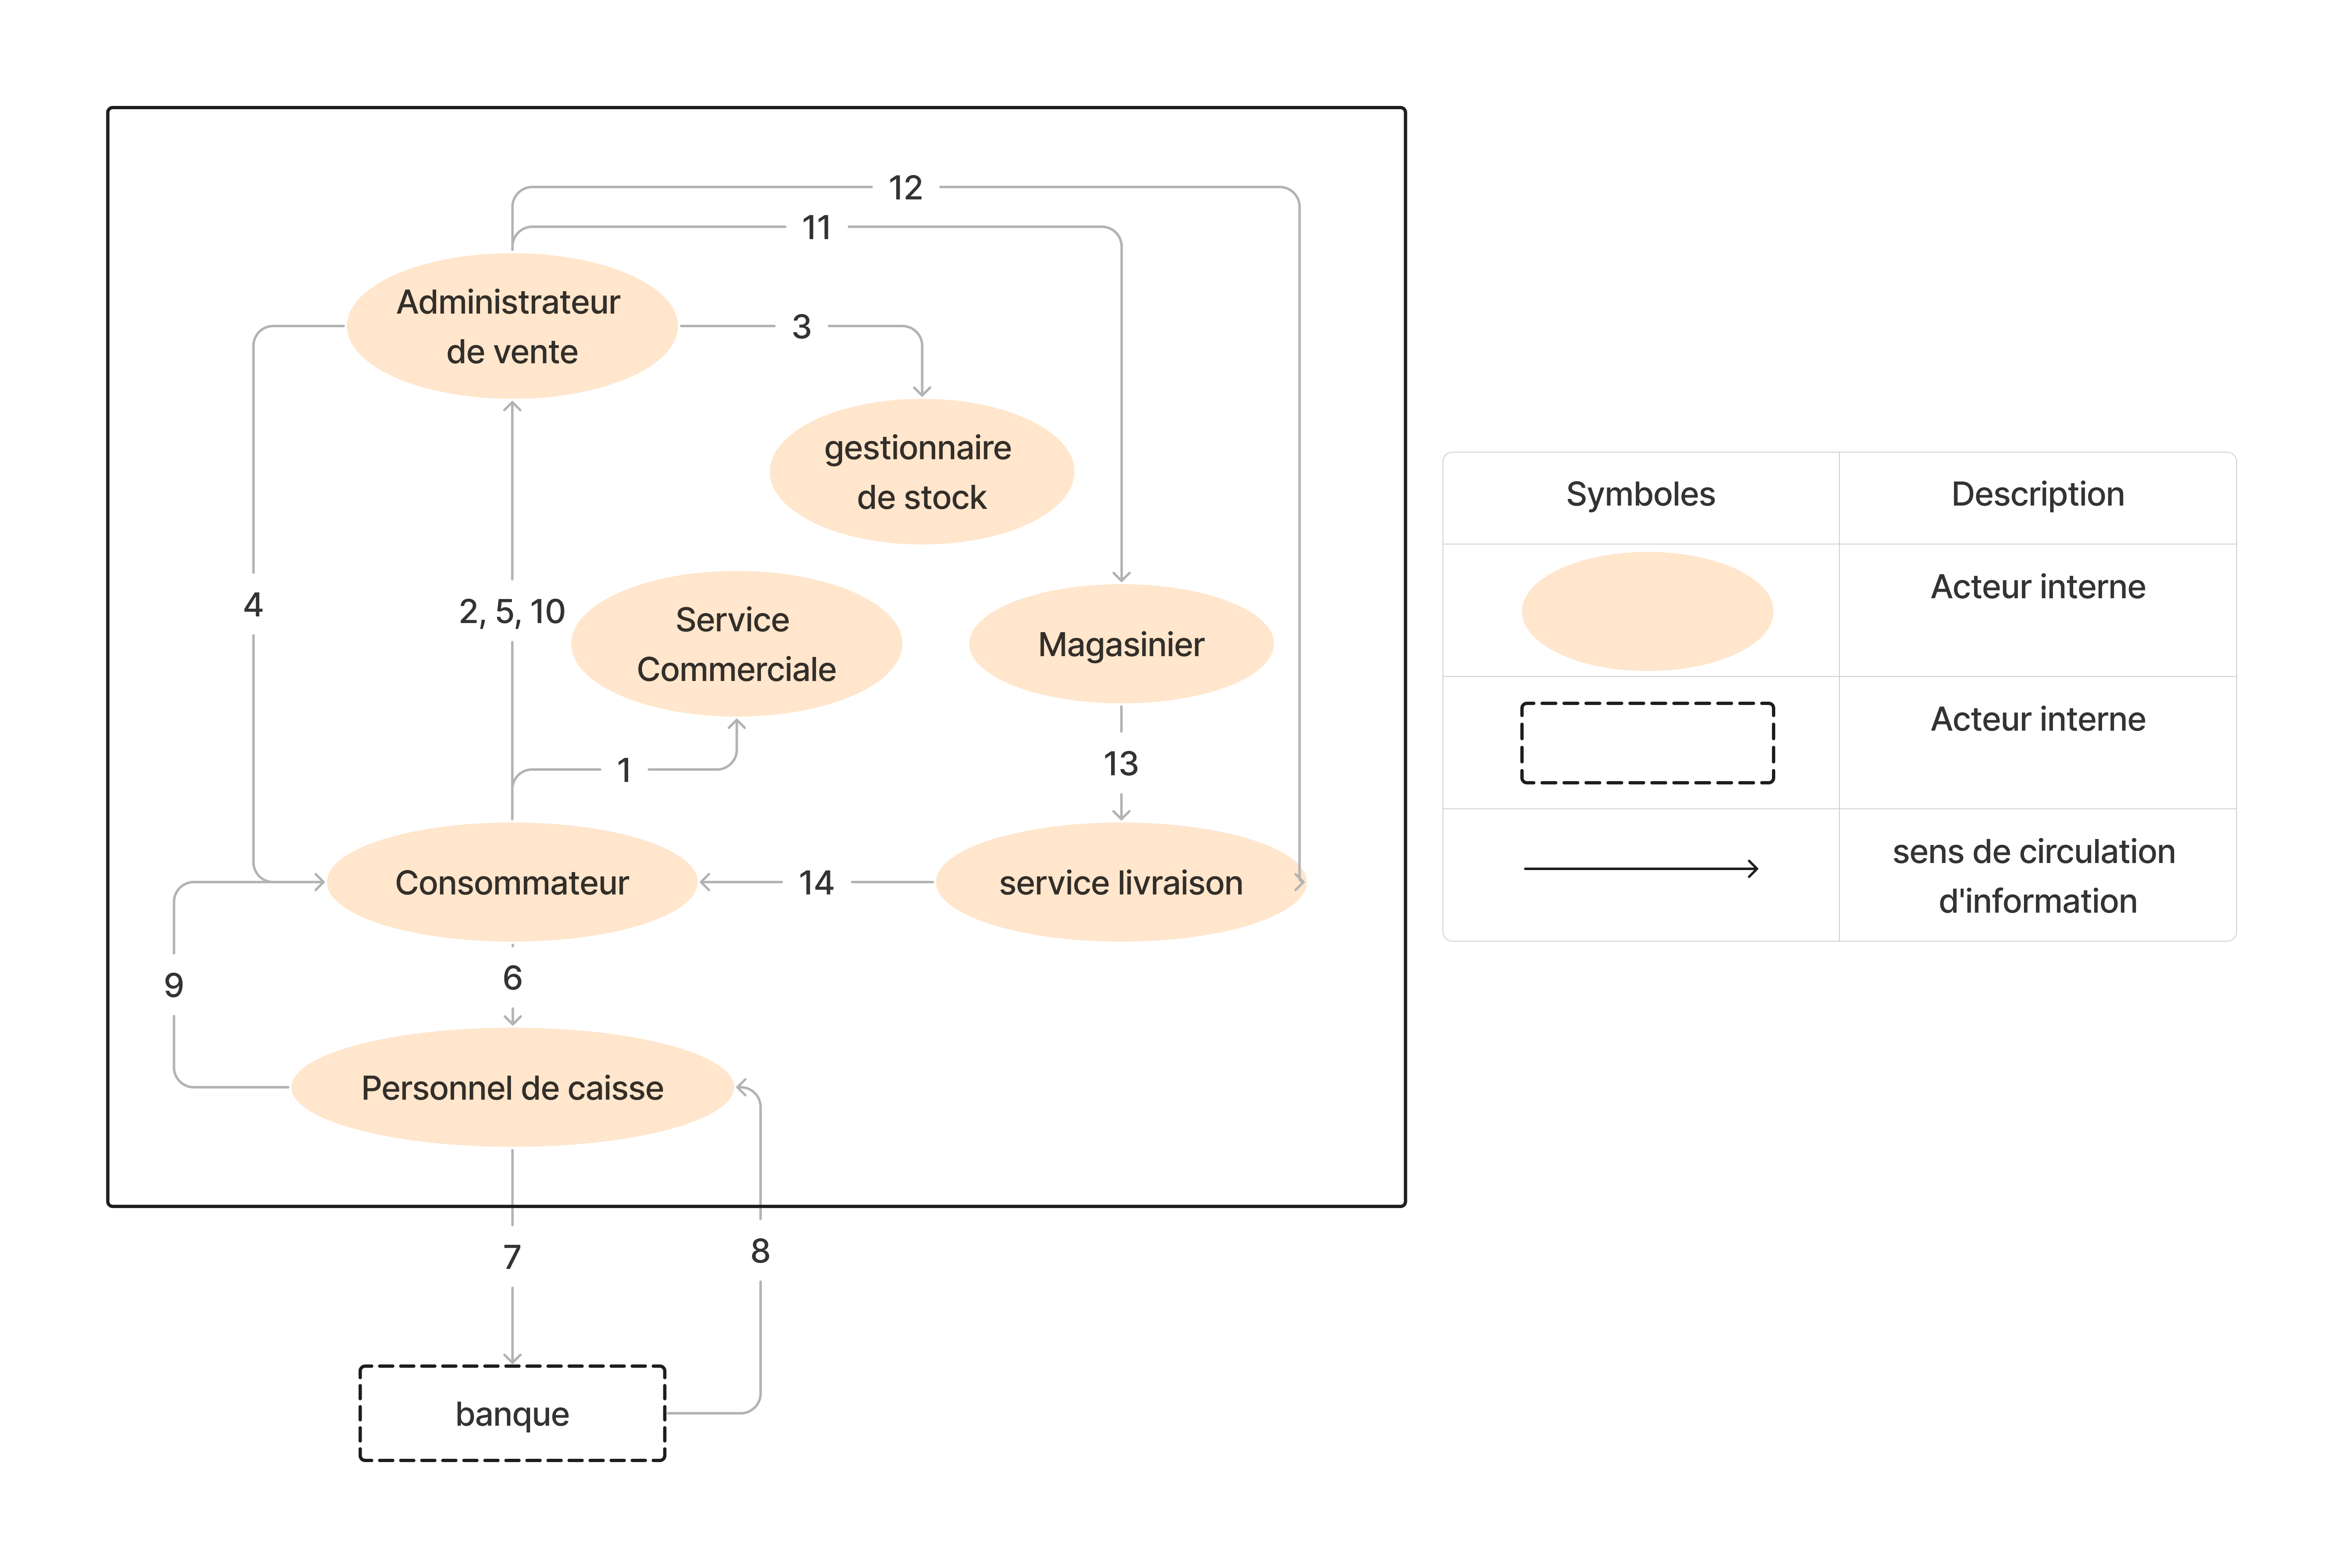
\includegraphics[width=0.8\textwidth]{images/Diagramme de flux.png}
\caption{Diagramme de flux de données}
\end{figure}
\textbf{1/}Recherche de marchandise , \textbf{2/}Demande de marchandises , \textbf{3/}Vérification de produit dans le stock , 
\textbf{4/}Obtention du la facture proforma , \textbf{5/}effectuer la commande , \textbf{6/}payement par cheque ou espèces
 , \textbf{7/}dépose de cheque , \textbf{8/}récupération de l’argent , \textbf{9/}Confirmation de payement
  , \textbf{10/}dipose de ticket de caisse , \textbf{11/}Ordre de chargement , \textbf{12/}Ordre de livraison
 \textbf{13/}chargement des marchandise , \textbf{14/}Expédition de commande

\section{Etude des procedures}
Cette étude permet de mieux comprendre l’enchaînement des tâches du domaine étudié et la circulation de l’information entre les différents postes de travail.
\newline La notation adoptée est la suivante
\begin{table}[h!]
    \centering
    \begin{tabular}{c}
        \centering
        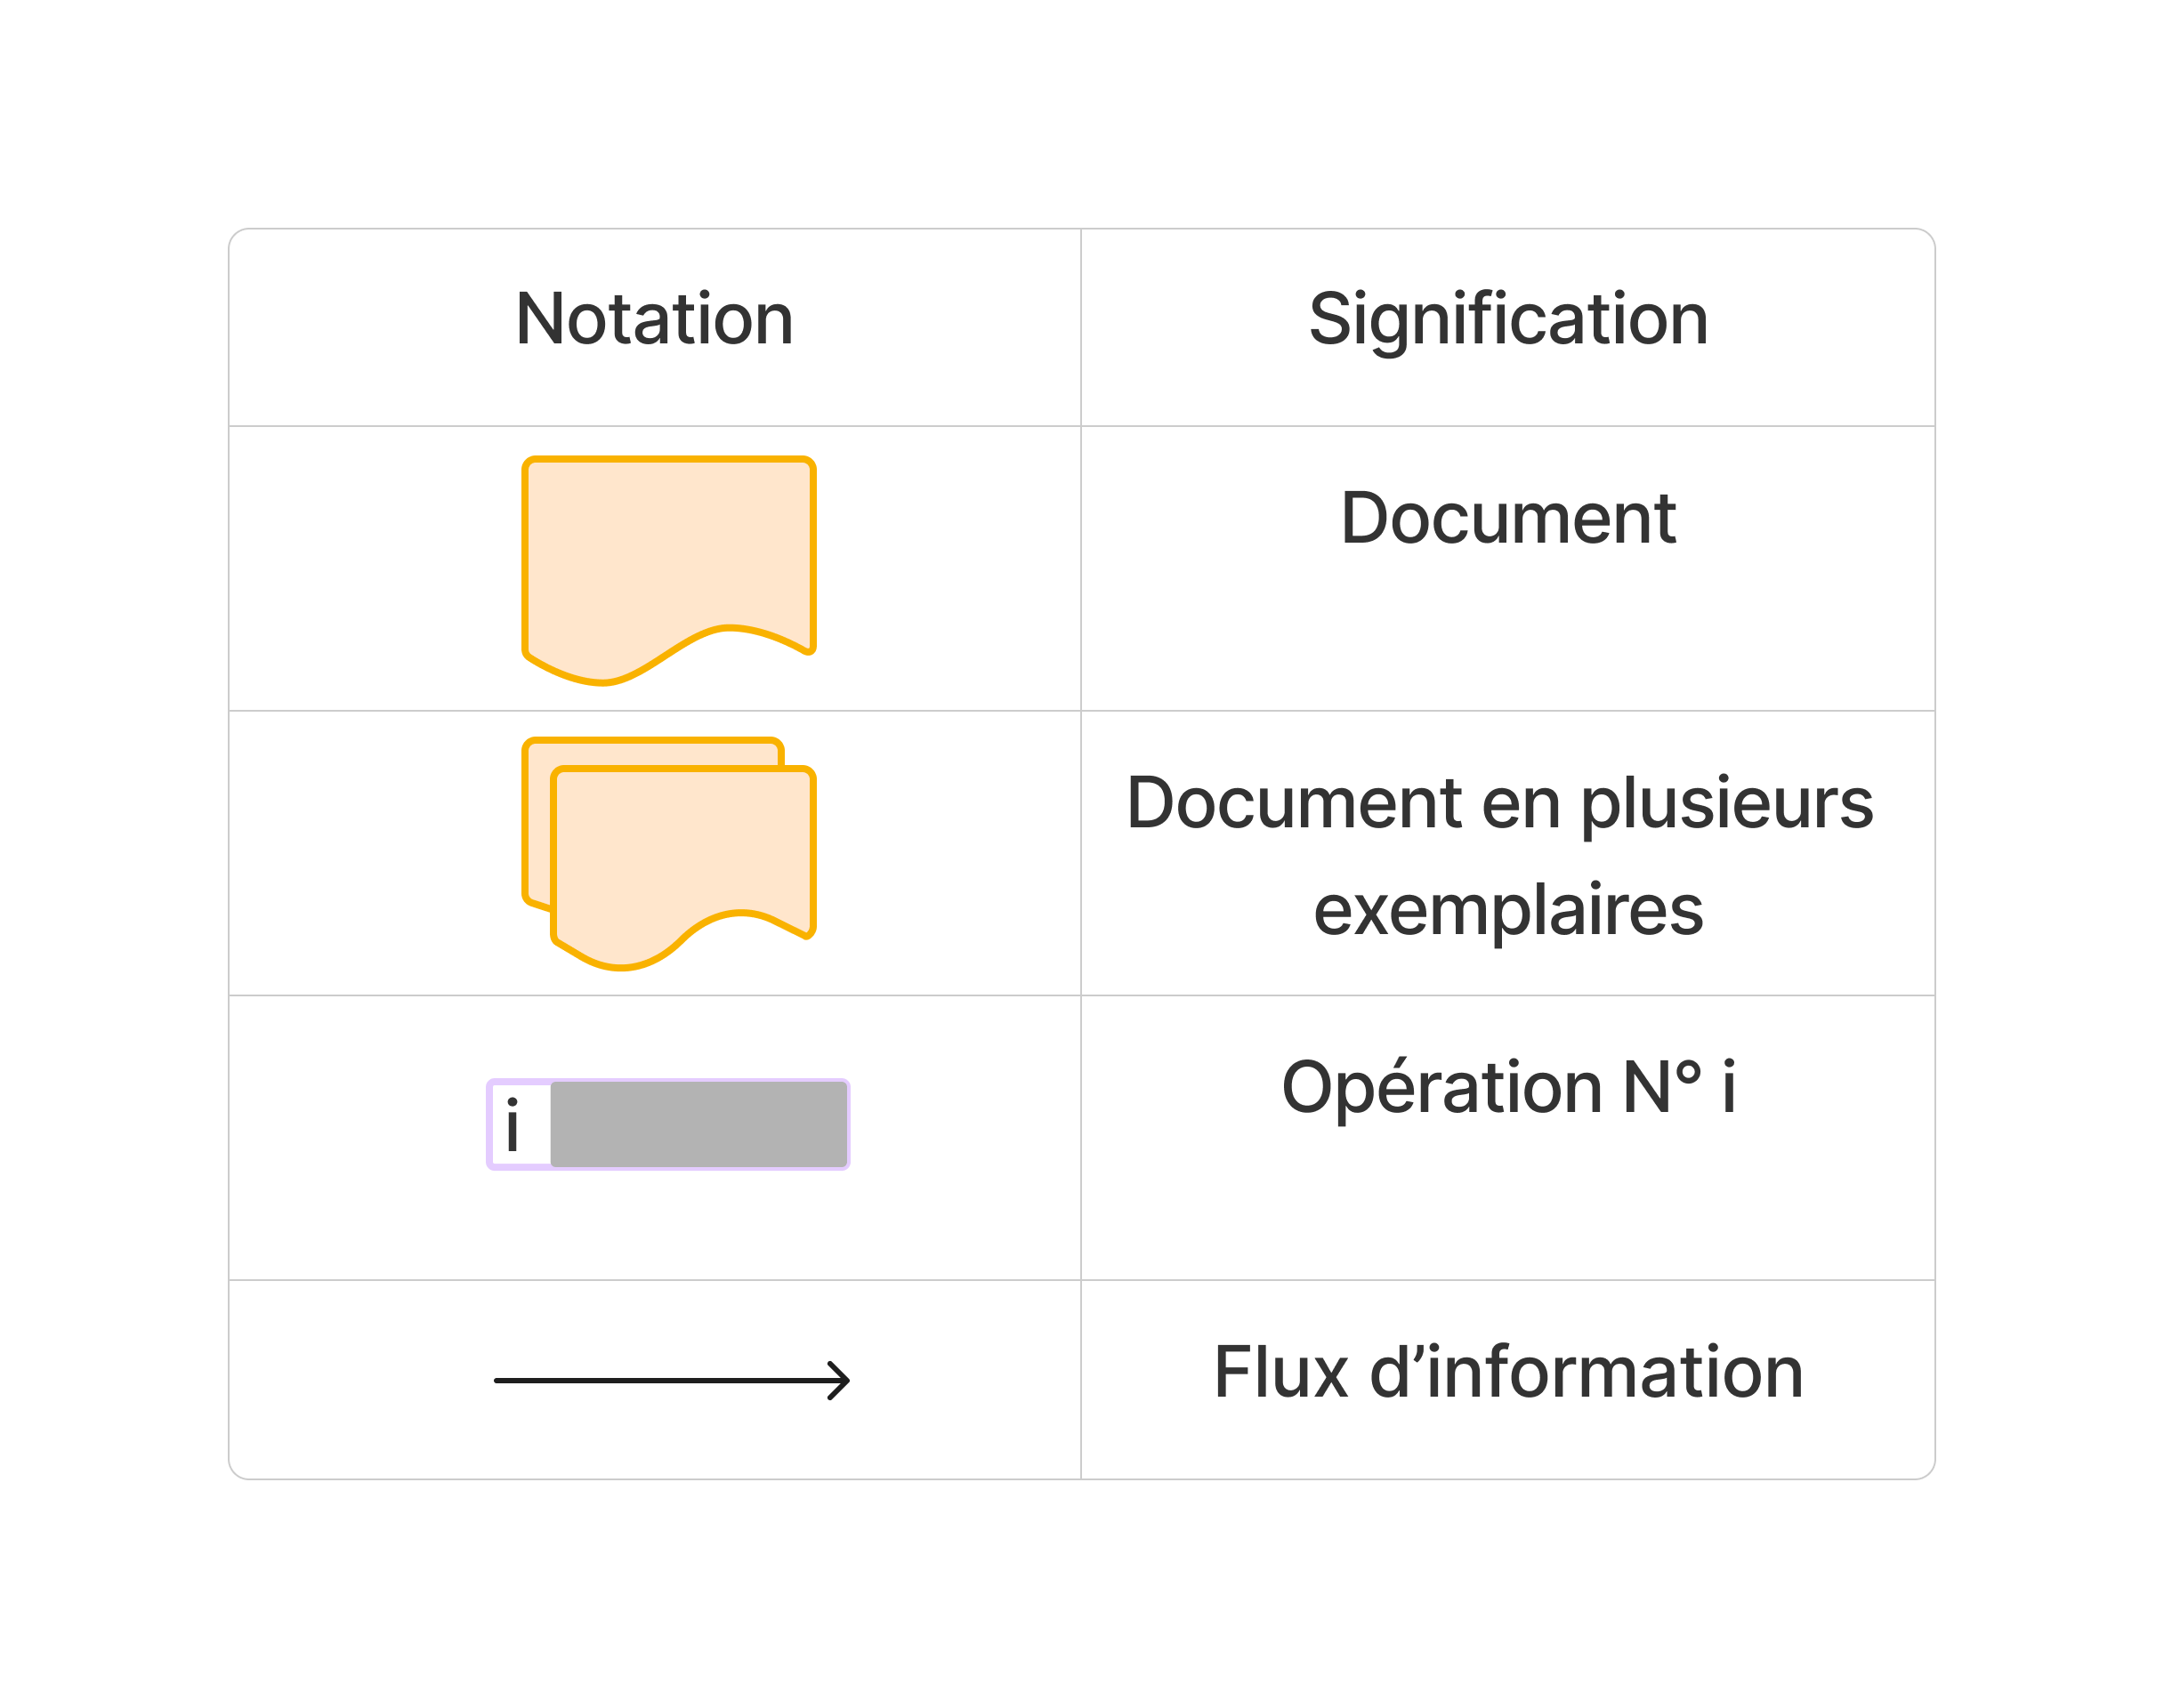
\includegraphics[width=0.5\textwidth]{images/description procedures.png}
    \end{tabular}
    \caption{Notations pour les procédures}
    \label{tab:Notations pour les procédures}
\end{table}
\subsection{Diagramme de procedures}
\begin{figure}[h!]\label{fig:procedures}
\centering
\includegraphics[width=0.7\textwidth]{images/Diagramme de procedures.png}
\caption{Diagramme de procedures}
\end{figure}
\subsection{Description des opérations}
\begin{table}[h!]
    \centering
    \begin{tabular}{|c|l|}
        \hline
        1 & \textbf{Prévente:}création de bon de commande \\
        2 & \textbf{Paiement:} \\
          & \textbf{- Cas1:}par cheque \\
          & \textbf{- Cas2:}par espéce \\
        3 & \textbf{Confirmation du paiement} \\
        4 & \textbf{Effectuer la vente: } \\
          & \textbf{-}l’envoie de facture de vente au consommateur. \\
          & \textbf{-}ordre le magasinier a chargé la marchandise. \\
        5 & \textbf{Livrer la commande au client} \\
        6 & \textbf{Confirmer la réception des marchandises} \\
       \hline
    \end{tabular}
    \caption{Description des opérations}
    \label{tab:auxiliaire Description des opérations}
\end{table}
\section{Étude documentaire}
\subsection{Définition d’un document }
Un document est un ensemble d'informations écrites, complètes et précises qui nous permettent de mener des opérations en vue d'une bonne gestion du domaine. Il existe deux types de documents :
\begin{itemize}
    \item Documents internes:Déterminés par le domaine d'études.
    \item Documents externes:Destinés au domaine d'études.
\end{itemize}
\subsection{Liste des documents}
Facture préforma, Bon de commande, Facture de vente, Bordereau de marchandises, Bon de livraison, Bon de réception, Reçu de paiement
\subsection{Tableau désignation des abréviations}
\begin{table}[h!]
    \centering
    \begin{tabular}{|c|c|}
    \hline
        type & Désignation \\
        \hline
        N & Numérique \\
        A & Alphabétique \\
        AN & Alphanumérique \\
        D & Date\\
        H & Heure \\
        S & Signature \\
        T & Text \\
        \hline
    \end{tabular}
    \caption{Tableau désignation des abréviations}
    \label{tab:désignation des abréviations}
\end{table}
\newpage
\subsection{Fiche d’étude de document N°1}
Désignation :facture préforma.
\newline Rôle :c’est utilisé pour les marchandises non destinées à la vente. Elle permet de déclarer la valeur et la nature de la marchandise sans pour autant avoir de valeur comptable
\newline Nature :interne
\newline Fréquence :par demande
\newline Émetteur :administrateur de vente
\newline Récepteur :consommateur \cite{Facturep}
\begin{table}[h!]
    \centering
    \begin{tabular}{|c|c|c|c|}
         \hline
\multicolumn{4}{|c|}{Analyse de contenu de document}\\
\hline
Contient rubriques & Type & Taille & Observation\\
\hline
 N° facture  & N & 10 & \\
 N° commande  & N & 10 & \\
 Nom entreprise & A & 20 & \\
 Adresse postale & AN & 100 & \\
 Adresse mail & AN & 100 & \\
 Téléphone & N & 10 & \\
Date & D & 8 & JJ/MM/AAAA \\
Nom consommateur & A & 20 & \\
Adresse postale consommateur & AN & 100 & \\
Adresse mail consommateur & AN & 100 & \\
Téléphone consommateur & N & 10 & \\
N° article & N & 10 & \\
Nom article & A & 20 & \\
Quantité & N & 10 & \\
Prix unitaire & N & 20 & \\
Prix totale d’article & N & 20 & \\
TTC & N & 20 & \\
Prix totale hors tax & N & 20 & \\
Prix totale avec tax & N & 20 & \\
Description d’article & AN & 100 & \\
\hline
    \end{tabular}
    \caption{Fiche d’étude de document N°1}
    \label{tab:1}
\end{table}
\newpage
\subsection{Fiche d’étude de document N°2}
Désignation :bon de commande.
\newline Rôle :les bons de commande sont émis par l’acheteur, qui veut s’assurer qu’il obtienne exactement ce qu’il a commandé
\newline Nature :externe
\newline Fréquence :
\newline Émetteur :consommateur
\newline Récepteur :administrateur de vente \cite{Bonc}
\begin{table}[h!]
    \centering
    \begin{tabular}{|c|c|c|c|}
         \hline
\multicolumn{4}{|c|}{Analyse de contenu de document}\\
\hline
Contient rubriques & Type & Taille & Observation\\
\hline
 N° facture  & N & 10 & \\
 N° commande  & N & 10 & \\
 Nom entreprise & A & 20 & \\
 Adresse postale & AN & 100 & \\
 Adresse mail & AN & 100 & \\
 Téléphone & N & 10 & \\
Date & D & 8 & JJ/MM/AAAA \\
Nom consommateur & A & 20 & \\
Adresse postale consommateur & AN & 100 & \\
Adresse mail consommateur & AN & 100 & \\
Téléphone consommateur & N & 10 & \\
N° article & N & 10 & \\
Nom article & A & 20 & \\
Quantité & N & 10 & \\
Prix unitaire & N & 20 & \\
Prix totale d’article & N & 20 & \\
TTC & N & 20 & \\
Prix totale hors tax & N & 20 & \\
Prix totale avec tax & N & 20 & \\
Description d’article & AN & 100 & \\
\hline
    \end{tabular}
    \caption{Fiche d’étude de document N°2}
    \label{tab:2}
\end{table}



\newpage
\subsection{Fiche d’étude de document N°3}
Désignation :facture de vente.
\newline Rôle :un document représentant la preuve comptable d'un achat ou d'une vente de produits ou de services.
\newline Nature :interne
\newline Fréquence :par demande
\newline Émetteur :administrateur de vente
\newline Récepteur :consommateur \cite{facturev}
\begin{table}[h!]
    \centering
    \begin{tabular}{|c|c|c|c|}
         \hline
\multicolumn{4}{|c|}{Analyse de contenu de document}\\
\hline
Contient rubriques & Type & Taille & Observation\\
\hline
 N° facture  & N & 10 & \\
 N commande  & N & 10 & \\
 Nom entreprise & A & 20 & \\
 Adresse postale & AN & 100 & \\
 Adresse mail & AN & 100 & \\
 Téléphone & N & 10 & \\
 N° registre commerce & AN & 10 & \\
 Fax & N & 9 & \\
Date & D & 8 & JJ/MM/AAAA \\
Nom consommateur & A & 20 & \\
Adresse postale consommateur & AN & 100 & \\
Adresse mail consommateur & AN & 100 & \\
Téléphone consommateur & N & 10 & \\
N° registre consommateur & AN & 10 & \\
Fax consommateur & N & 9 & \\
N° article & N & 10 & \\
Nom article & A & 20 & \\
Quantité & N & 10 & \\
Prix unitaire & N & 20 & \\
Prix totale d’article & N & 20 & \\
TTC & N & 20 & \\
Prix totale hors tax & N & 20 & \\
Prix totale avec tax & N & 20 & \\
Description d’article & AN & 100 & \\
\hline
    \end{tabular}
    \caption{Fiche d’étude de document N°3}
    \label{tab:3}
\end{table}


\newpage
\subsection{Fiche d’étude de document N°4}
Désignation :bordereau des marchandises.
\newline Rôle :un bordereau de marchandises présente les lignes d'expédition emballées prêtes pour l'expédition.
\newline Nature :interne
\newline Fréquence :par demande
\newline Émetteur :administrateur de vente
\newline Récepteur :magasinier\cite{bordereau}
\begin{table}[h!]
    \centering
    \begin{tabular}{|c|c|c|c|}
         \hline
\multicolumn{4}{|c|}{Analyse de contenu de document}\\
\hline
Contient rubriques & Type & Taille & Observation\\
\hline
 N° facture  & N & 10 & \\
 N° commande  & N & 10 & \\
 Nom entreprise & A & 20 & \\
 Adresse postale & AN & 100 & \\
 Adresse mail & AN & 100 & \\
 Téléphone & N & 10 & \\
Date & D & 8 & JJ/MM/AAAA \\
Nom consommateur & A & 20 & \\
Adresse postale consommateur & AN & 100 & \\
Adresse mail consommateur & AN & 100 & \\
Téléphone consommateur & N & 10 & \\
N° article & N & 10 & \\
Nom article & A & 20 & \\
Quantité & N & 10 & \\
Prix unitaire & N & 20 & \\
Prix totale d’article & N & 20 & \\
TTC & N & 20 & \\
Prix totale hors tax & N & 20 & \\
Prix totale avec tax & N & 20 & \\
Description d’article & AN & 100 & \\
\hline
    \end{tabular}
    \caption{Fiche d’étude de document N°4}
    \label{tab:4}
\end{table}


\newpage
\subsection{Fiche d’étude de document N°5}
Désignation :bon de livraison.
\newline Rôle :le bon de livraison est un document signé par la personne qui réceptionne une marchandise et la vérifie
\newline Nature :interne
\newline Fréquence :par demande
\newline Émetteur :administrateur de vente
\newline Récepteur :service livraison \cite{bonl}
\begin{table}[h!]
    \centering
    \begin{tabular}{|c|c|c|c|}
         \hline
\multicolumn{4}{|c|}{Analyse de contenu de document}\\
\hline
Contient rubriques & Type & Taille & Observation\\
\hline
 N° facture  & N & 10 & \\
 N° commande  & N & 10 & \\
 Nom entreprise & A & 20 & \\
 Adresse postale & AN & 100 & \\
 Adresse mail & AN & 100 & \\
 Téléphone & N & 10 & \\
Date & D & 8 & JJ/MM/AAAA \\
Nom consommateur & A & 20 & \\
Adresse postale consommateur & AN & 100 & \\
Adresse mail consommateur & AN & 100 & \\
Téléphone consommateur & N & 10 & \\
N° article & N & 10 & \\
Nom article & A & 20 & \\
Quantité & N & 10 & \\
Prix unitaire & N & 20 & \\
Prix totale d’article & N & 20 & \\
TTC & N & 20 & \\
Prix totale hors tax & N & 20 & \\
Prix totale avec tax & N & 20 & \\
Description d’article & AN & 100 & \\
\hline
    \end{tabular}
    \caption{Fiche d’étude de document N°5}
    \label{tab:5}
\end{table}


\newpage
\subsection{Fiche d’étude de document N°6}
Désignation :bon de reception.
\newline Rôle :le bon de réception est le document que le consemmateur remettez au livreur, ou que vous transmettez au fournisseur, pour accuser bonne réception, ou pas, de la marchandise que vous lui aviez commandée.
\newline Nature :externe
\newline Fréquence :
\newline Émetteur :consommateur
\newline Récepteur :service livraison \cite{bonr}
\begin{table}[h!]
    \centering
    \begin{tabular}{|c|c|c|c|}
         \hline
\multicolumn{4}{|c|}{Analyse de contenu de document}\\
\hline
Contient rubriques & Type & Taille & Observation\\
\hline
 N° facture  & N & 10 & \\
 N° commande  & N & 10 & \\
 Ordre d’exécution N° & N & 10 & \\
 Nom entreprise & A & 20 & \\
 Adresse postale & AN & 100 & \\
 Adresse réception & AN & 100 & \\
Date réception & D & 8 & JJ/MM/AAAA \\
Nom consommateur & A & 20 & \\
Nom de l'expéditeur & A & 20 & \\
Adresse mail consommateur & AN & 100 & \\
Montant de la facture & N & 20 & \\
montant payé d'avance & N & 20 & \\
montant en caisse & N & 20 & \\
N° article & N & 10 & \\
Nom article & A & 20 & \\
Quantité & N & 10 & \\
Prix unitaire & N & 20 & \\
Prix totale d’article & N & 20 & \\
TTC & N & 20 & \\
Prix totale hors tax & N & 20 & \\
Prix totale avec tax & N & 20 & \\
Description d’article & AN & 100 & \\
condition d’article & AN & 100 & \\
commentaires & AN & 100 & \\
\hline
    \end{tabular}
    \caption{Fiche d’étude de document N°6}
    \label{tab:6}
\end{table}
\newpage
\subsection{Fiche d’étude de document N°7}
Désignation :reçu de paiement.
\newline Rôle :un reçu de paiement est un document qui atteste d'une transaction financière. Il confirme la réception d'une somme d'argent ou d'une autre forme de paiement
\newline Nature :interne
\newline Fréquence :
\newline Émetteur :personal de caisse
\newline Récepteur :consommateur \cite{reçu}
\begin{table}[h!]
    \centering
    \begin{tabular}{|c|c|c|c|}
         \hline
\multicolumn{4}{|c|}{Analyse de contenu de document}\\
\hline
Contient rubriques & Type & Taille & Observation\\
\hline
 N° reçu de paiement & N & 10 & \\
 N° commande  & N & 10 & \\
 Nom entreprise & A & 20 & \\
 Nom personnel de caisse & A & 20 & \\
 Date de paiement & D & 8 & JJ/MM/AAAA \\
Nom consommateur & A & 20 & \\
montant payé & N & 20 & \\
type de paiement & AN & 100 & \\
\hline
    \end{tabular}
    \caption{Fiche d’étude de document N°7}
    \label{tab:7}
\end{table}
\section{Étude des acteurs de l'écosystème commercial}
On définie d’abord L’acteur principale dans notre projet qui selon les lois nationales est réportorié sous le terme Agent économique
\subsection{Consommateur}
Toute personne physique ou morale qui acquiert ou utilise, à des fins excluant tout caractère professionnel, des biens ou des services mis en vente ou offerts.\cite{Consommateur}  
\subsection{Service commerciale}
Le service commercial est l’ensemble des activités ayant pour objet la vente et/ou la promotion d’un produit ou d’un service. Il s’agit donc du lien entre l’entreprise et ses clients potentiels ou existants.
\cite{Service}\newline\textbf{Les missions du service commercial}\newline
\begin{itemize}
    \item [•]   Le service commercial a pour mission principale de générer des revenus pour l’entreprise en mettant en œuvre une stratégie commerciale efficace. Il doit également assurer le suivi des clients et des prospects, afin de les fidéliser et de les inciter à acheter les produits ou les services de l’entreprise
    \item [•]	Pour ce faire, le service commercial doit mettre en place une bonne communication avec les autres services de l’entreprise, notamment la production et la logistique, afin de garantir la bonne exécution des commandes. Il doit également collaborer étroitement avec le service marketing, afin de définir les meilleures offres commerciales et d’assurer une bonne promotion des produits.
    \item [•]   En outre, le service commercial est chargé de gérer les relations avec les fournisseurs, afin de négocier les meilleurs prix et conditions de livraison. Il doit également veiller à ce que les produits soient conformes aux normes et aux réglementations en vigueur.
    \item [•]   Enfin, le service commercial doit assurer un suivi régulier de la concurrence, afin d’identifier les menaces et les opportunités potentielles pour l’entreprise.
\end{itemize}
\subsection{Gestionnaire de stock}
Il gère et optimise la gestion des stocks (entrées et sorties des marchandises) pour minimiser le niveau de stocks sans risquer la rupture. En liaison étroite avec les fournisseurs et les transporteurs, il conçoit et coordonne l'ensemble de la chaîne d'approvisionnement dans les délais impartis. Il met en place le stockage des produits (surface, rangement, rotation des produits) en fonction des services commerciaux et de la demande des clients. Il supervise le traitement des commandes en veillant au respect des coûts et des délais. Il est le garant de la disponibilité des marchandises.
\cite{Gestionnaire}\newline\textbf{Les missions du Gestionnaire de stock}\newline
\begin{itemize}
    \item [•] Planifier les livraisons avec les fournisseurs en fonction de divers critères (type d'emballages, quantité, fréquence de tournées des camions)
    \item [•]	Suivre les critères de performance des fournisseurs (délais de livraison, niveaux de qualité, respect des conditions négociées par l'entreprise)
    \item [•]   Contrôler qualitativement et quantitativement les marchandises réceptionnées
    \item [•]   Négocier des solutions de rechange avec les fournisseurs en cas de dysfonctionnement, parfois dans l'urgence
    \item [•]   Suivre les ventes et les prévisions pour assurer la disponibilité des produits et superviser la préparation des commandes.
\end{itemize}
\subsection{Personnel de caisse }
Le caissier est chargé de gérer les transactions financières avec les clients. Cela comprend l'enregistrement des achats et la manipulation des paiements. Le caissier doit maintenir la précision des registres comptables, offrir un service clientèle efficace et contribuer à assurer un flux monétaire régulier au sein du grossiste.
\cite{Personnel}\newline\textbf{Les missions du Personnel de caisse}\newline
\begin{itemize}
    \item [•] Enregistrement précis des achats, émission des factures et traitement des paiements.
    \item [•] Maintien de la précision des informations financières pour assurer une comptabilité correcte.
    \item [•] Fourniture d'un service clientèle efficace en répondant aux questions des clients et en facilitant leurs besoins financiers liés aux achats.
    \item [•] Contribution à maintenir un flux monétaire régulier au sein du grossiste pour garantir le bon fonctionnement financier de l'entreprise.
\end{itemize}
\subsection{Administrateur des ventes}
L’administrateur des ventes (ADV) organise ou réalise la gestion des contrats de vente depuis la réception des commandes jusqu'à la livraison des produits chez le client. Il s’assure de la bonne exécution des commandes clients, réceptionne la marchandise, organise l’acheminement et assure le suivi du traitement des commandes auprès des clients. Il réalise l'interface entre les clients, les services internes (commercial, production, planification) et les intervenants externes de l'entreprise (fournisseurs, transporteurs).
\cite{Administrateur}\newline\textbf{Les missions du  Administrateur des ventes}\newline
\begin{itemize}
    \item [•] Définir des procédures administratives de traitement des commandes 
    \item [•] Proposer des axes d'amélioration 
    \item [•] Contrôler l'application des procédures de commande 
    \item [•] Etablir un contrat de vente 
    \item [•] Elaborer un planning de production
    \item [•] Planifier le traitement des commandes 
    \item [•] Déclencher un ordre de production et le transmettre au service concerné 
    \item [•] Suivre l'état d'avancement de la fabrication d'un produit 
    \item [•] Analyse statistique
    \item [•] Droit commercial
    \item [•] Réglementation des douanes
    \item [•] Management
    \item [•] Organisation de la chaîne logistique
    \item [•] Méthodes d'approvisionnement
    \item [•] Gestion des stocks et des approvisionnements
    \item [•] Gestion financière
    \item [•] Gestion budgétaire
\end{itemize}
\subsection{Magasinier}
Le magasinier assure le suivi des livraisons et de l’état des stocks pour éviter toute rupture dans la chaîne logistique.La préparation de commandes n’a aucun secret pour le magasinier ! Ce professionnel de la logistique est le garant des stocks d’un entrepôt, d’une usine ou d’une entreprise. Au quotidien, il réceptionne les commandes, les vérifie et les affecte aux bons rayons de stockage. Il peut aussi préparer les commandes en s’appuyant sur les bordereaux de commande, sous la responsabilité du chef magasinier.
\cite{Magasinier}\newline
\textbf{Les missions du Magasinier}\newline
\begin{itemize}
    \item [•]Réceptionner une livraison (marchandise à l’unité, en lot ou en palettes),
    \item [•] Vérifier la conformité de la livraison.
    \item [•] Lire un plan de stockage pour répartir les livraisons.
    \item [•] Préparer une commande.
    \item [•] Réaliser le prélèvement de produits selon les instructions de préparation de commande et constituer les colis ou lots à expédier,
    \item [•] Utiliser des engins de manutention non motorisés (transpalette, diable) ou nécessitant une habilitation comme le CACES (certificat d’aptitude à la conduite en sécurité).
    \item [•] Charger des marchandises.
    \item [•] Acheminer des marchandises en zone d'expédition, de stockage ou de production.
    \item [•] Renseigner les supports de suivi de commande,
    \item [•] Transmettre un état des produits détériorés et du matériel défectueux.
\end{itemize}
\subsection{Service de livraison}
Le service de livraison d'une entreprise, souvent qualifié de service de distribution, constitue l'élément fondamental de la logistique et des opérations. Sa mission essentielle est de coordonner le transfert des produits de l'entreprise depuis leurs points de stockage ou de production jusqu'aux destinataires ultimes, que ce soient les clients, les points de vente ou d'autres partenaires commerciaux. Axé sur l'optimisation de la circulation des marchandises, ce service s'engage à respecter des normes élevées en matière de fiabilité, de rapidité et de sécurité à chaque étape du processus de distribution.
\cite{logistique}\newline\textbf{Les missions du Service de livraison}\newline
\begin{itemize}
    \item [•] Acheminer les produits de l'entreprise vers les clients et les points de vente.
    \item [•] Assurer une gestion efficace de la chaîne d'approvisionnement. 
    \item [•] Planifier et optimiser les itinéraires de livraison. 
    \item [•] Surveiller les expéditions en temps réel. 
    \item [•] Réaliser des livraisons rapides et efficientes. 
    \item [•] Assurer la sécurité des produits pendant le transport. 
    \item [•] Prioriser la satisfaction client en offrant un service fiable et sécurisé.
\end{itemize}




\section{l'exemple d'application existant(logiciel de gestion du stock(Djawahirsoft))}
\subsubsection{Description}
Djawahirsoft est un logiciel de gestion qui simplifie la gestion commerciale et des stocks. Il permet de créer des devis, commandes, factures, bons de livraison et bons de réception. Il gère les inventaires, les régularisations de stock, ainsi que les règlements clients et fournisseurs.\cite{Djawahirsoft}\subsubsection{Les fonctionnalités:}
\begin{itemize}
    \item [•] Gestion des comptes. 
    \item [•] Gestion des produits/services.
    \item [•] Gestion des clients/fournisseurs.
    \item [•] Gestion des dépôts et stock.
    \item [•] Gestion des familles (produit, service,client).
    \item [•] importation et exportation des données.
    \item [•] Devis/Facture proforma, bons de livraisons, factures d'achats et bons de réceptions, factures de ventes, avoirs clients et fournisseurs.
    \item [•] Gestion des commandes fournisseurs/clients
    \item [•] Gestion d'échéanciers de paiements des factures de vente et d'achat
    \item [•] Consulter et suivre les Arrivage des produits.
    \item [•] gérer les règlements et remboursement clients/fournisseurs.
    \item [•] gestion des charges et dépenses
    \item [•] Transferts de stock inter-dépôts.
    \item [•] Calculer et consulter les bénéfices et les chiffres d'affaires (par produit, par jour, par client).
\end{itemize}
Djawehrsoft est un logiciel de gestion de stock traditionnel qui ne suit pas les avancées technologiques et ne répond pas aux exigences actuelles du marché, telles que la gestion et la vérification des stocks à distance,par ailleurs, il ne dispose pas de fonctionnalités modernes comme les notifications en temps réel, l'intégration avec les plateformes de commerce électronique, et les outils d'analyse de données avancés, dont le vendeur moderne a un besoin crucial pour développer son activité et optimiser sa gestion.
\section{Problématique}
Le secteur commercial en Algérie est confronté à de nombreux défis en raison d'une interconnectivité limitée entre les principaux acteurs : les grossistes, les détaillants et les entreprises. Ce manque de communication et de coordination entraîne plusieurs problèmes :
\begin{enumerate}
    \item \textbf{Difficultés d'approvisionnement pour les détaillants:}Les détaillants peinent à trouver les produits nécessaires en raison d'un réseau limité, ce qui perturbe la distribution efficace des marchandises et conduit à des pénuries ou à des retards.
    \item \textbf{Problèmes de stock chez les grossistes:}Les grossistes ont du mal à identifier et à comprendre les besoins spécifiques des détaillants, ce qui peut entraîner des surplus de stock ou des pénuries.
    \item \textbf{Complexité de trouver des sources fiables pour les entreprises:}Les entreprises rencontrent des obstacles pour localiser les grossistes répondant à leurs besoins spécifiques, ce qui complique leurs opérations d'approvisionnement.
    \item \textbf{Manque de transparence des prix:}Les prix des produits varient considérablement entre différents fournisseurs, compliquant la comparaison et la négociation pour les détaillants et les entreprises.
    \item \textbf{Difficulté de suivre les transactions et les performances des fournisseurs:}Les acteurs du secteur ont une visibilité limitée sur l'historique des transactions et les performances des fournisseurs et partenaires commerciaux.
    \item \textbf{Problèmes de gestion des promotions et des offres spéciales:}Les grossistes ont des difficultés à gérer et à communiquer efficacement les promotions et les offres spéciales aux détaillants.
    \item \textbf{Difficultés de suivi des tendances marché (Prix/Produits):}Les fournisseurs éprouvent des difficultés à garantir la disponibilité constante des produits dans les régions intérieures, entraînant des défis logistiques et des fluctuations d'approvisionnement pour les consommateurs locaux.
    \item \textbf{Indisponibilité des produits en Wilayas internes:}Pointe les difficultés d'approvisionnement rencontrées dans plusieurs régions internes, exposant ainsi les défis logistiques et économiques engendrés par cette situation.
\end{enumerate}
\section{Solution}
Pour répondre à ces défis, nous proposons une solution intégrée basée sur une plateforme Web intelligente, conçue pour améliorer l'interconnectivité et la gestion de l'écosystème commercial en Algérie. Voici les fonctionnalités et avantages spécifiques pour chaque type d'acteur
\subsection{Pour les grossistes}
\begin{itemize}
    \item [•] \textbf{Gestion des documents:}une fois qu'une commande est confirmée sur la plateforme Web, le logiciel de gestion des stocks génère automatiquement un bon de commande.
    \item [•] \textbf{Publication en temps réel:}Possibilité de publier instantanément des offres et des demandes de produits, créant un flux d'informations en temps réel.
    \item [•] \textbf{Gestion de stock optimisée:}Un logiciel de gestion de stock amélioré et connecté à la plateforme pour suivre et gérer les stocks de manière plus efficace.
    \item [•] \textbf{Liquidation des surplus:}Diffusion des offres de surplus de produits directement sur la plateforme, accessible à tous les détaillants et autres grossistes.
    \item [•] \textbf{Gestion des promotions:}Un module dédié pour créer, lancer et suivre les promotions et offres spéciales, avec une visibilité instantanée pour les détaillants.
\end{itemize}
\subsection{Pour les détaillants}
\begin{itemize}
    \item [•] \textbf{Accessibilité directe aux grossistes:}Cette fonctionnalité offre aux utilisateurs la possibilité de contacter directement un large éventail de fournisseurs en gros, simplifiant ainsi le processus d'approvisionnement et favorisant une meilleure connectivité dans le secteur.
    \item [•] \textbf{Facilité d'approvisionnement:}Accès à une plateforme dédiée où les demandes spécifiques de produits peuvent être diffusées et visualisées par tous les grossistes.
    \item [•] \textbf{Comparaison des prix:}Un outil pour comparer les prix des produits entre différents fournisseurs et régions en temps réel.
    \item [•] \textbf{Suivi des partenaires commerciaux et des évaluations:}Un tableau de bord permettant d'évaluer les performances des partenaires commerciaux et de suivre les évaluations des autres détaillants.
    \item [•] \textbf{Vente rapide et transparente:}Cette fonctionnalité permet aux utilisateurs de passer rapidement et facilement des commandes en toute transparence, depuis la recherche de produits jusqu'à la gestion des commandes, offrant ainsi une expérience d'achat fluide et efficace.
\end{itemize}
\subsection{Pour les entreprises}
\begin{itemize}
    \item [•] \textbf{Élargissement du réseau de contacts:}Une plateforme qui facilite l'expansion du réseau de contacts, augmentant les chances de trouver des sources fiables pour les produits nécessaires.
    \item [•] \textbf{Professionnalisme et qualité assurée:}Assurez la qualité des produits et le traitement adéquat des clients en travaillant avec des vendeurs vérifiés.
\end{itemize}
\phantom{hassane}
\newline
Cette solution intégrée offre une expérience complète et efficace, connectant de manière transparente la gestion des stocks et les interactions commerciales, pour créer un écosystème commercial dynamique et collaboratif en Algérie.
\section{Conclusion}
Ce chapitre a défini l'écosystème commercial et analysé les flux d'information, les procédures, et les rôles des acteurs. Nous avons identifié les problématiques et proposé des solutions pour améliorer l'efficacité de cet écosystème.
\newline \newline
Le schéma ci-dessous \ref{sx} illustre les interactions entre les différents acteurs et outils de l'écosystème commercial, montrant comment les données circulent entre l'acheteur, les applications, le site web, le logiciel, et le vendeur.
\begin{figure}[h!]
    \centering
    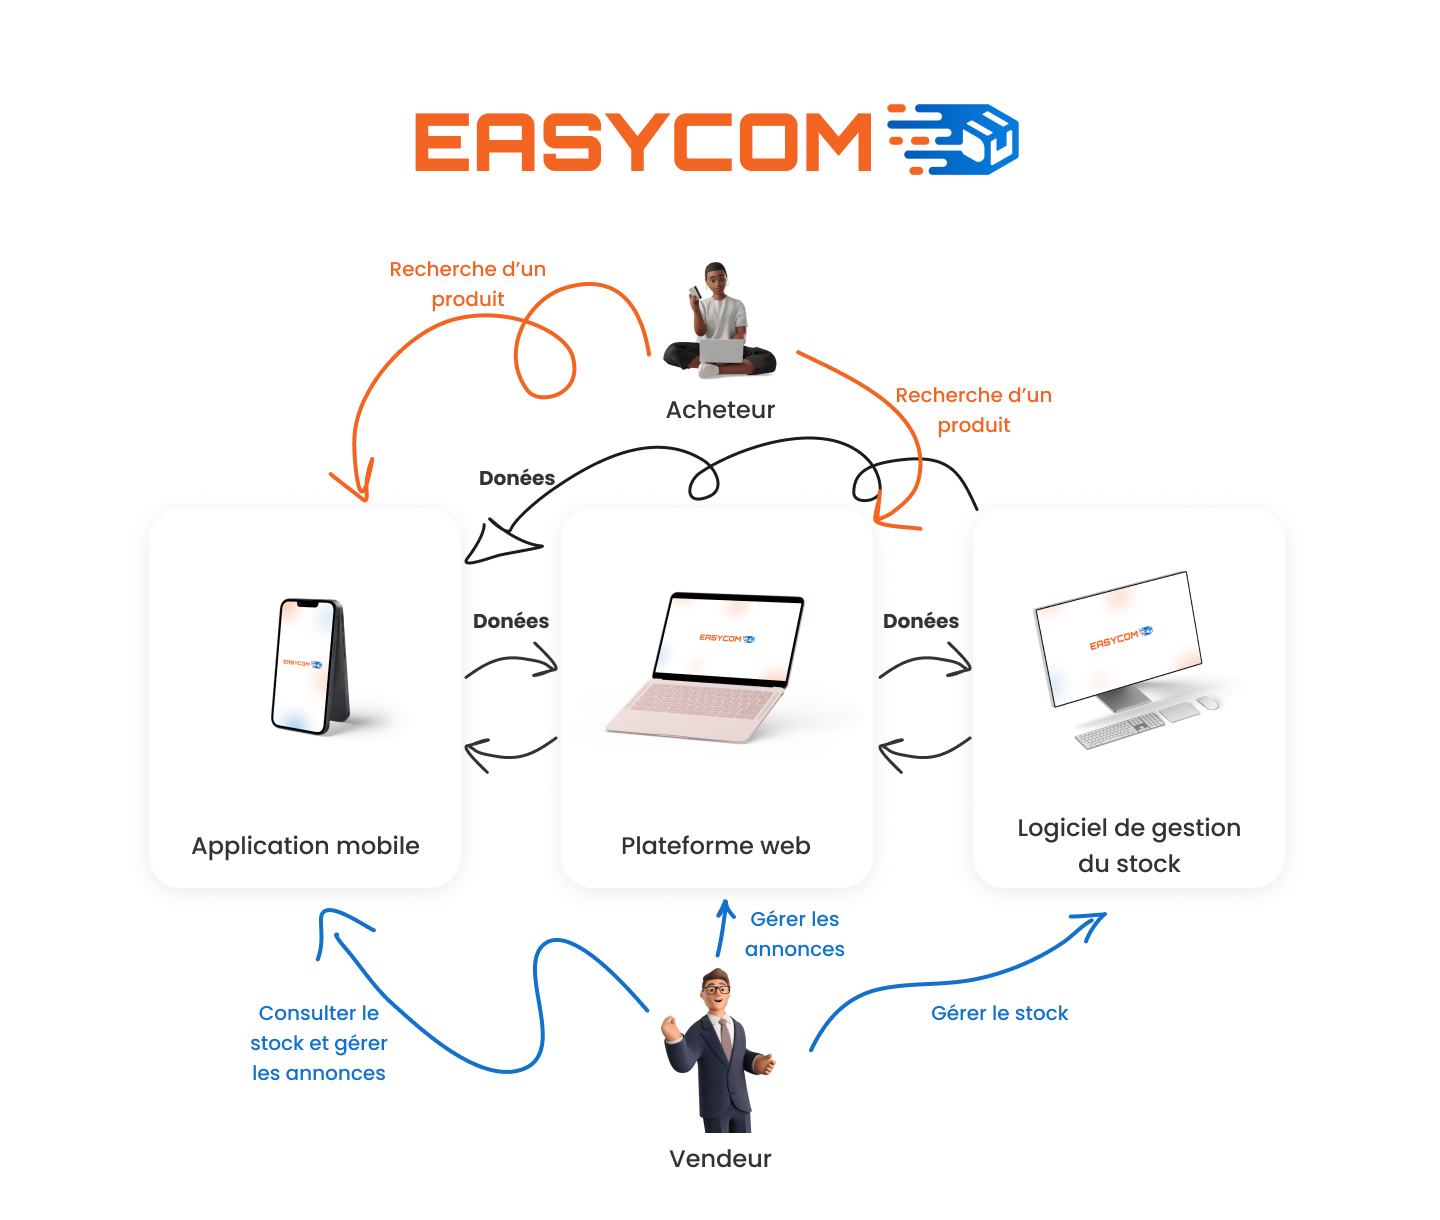
\includegraphics[width=1\textwidth]{images/photo_2024-06-05_16-41-28.jpg}
    \caption{Schéma expliquant notre système}
\end{figure}\label{sx}
%===================================================



\part{Platforme web et application mobile}
\chapter{Expresion des besoins}  
\newpage
\section{Introduction }
L'expression des besoins est la première étape fondamentale du projet. Ce chapitre se concentre sur l'identification et la documentation des besoins des utilisateurs et des parties prenantes. En utilisant des techniques telles que les diagrammes de cas d'utilisation et de séquence, nous décrivons les interactions entre les utilisateurs et le système. Ces outils visuels permettent de clarifier les fonctionnalités requises, les scénarios d'utilisation et les attentes des utilisateurs, jetant ainsi les bases pour une conception efficace et une mise en œuvre réussie.
\section{Spécification des besoins}
Cette étape porte sur la compréhension du contexte du système dans lequel nous déterminerons les besoins de notre solution.

Nous avons deux types de besoins : des besoins fonctionnels et des besoins non fonctionnels
\subsection{Les besoins fonctionnels }
Notre platforme "EASYCOM" offre un ensemble de fonctionnalités :
\begin{itemize}
    \item \textbf{Gestion des annonces:}les vendeurs est acheteurs peuvent créer, modifier et supprimer leurs annonces, tandis que les utilisateurs peuvent les suivre et interagir avec elles.
    \item \textbf{Gestion de profil:}Les utilisateurs, qu'ils soient vendeurs ou acheteurs, peuvent mettre à jour leurs informations personnelles et paramètres de compte.
    \item \textbf{Gestion de recherche:}La plateforme offre une recherche avancée selon divers critères pour trouver rapidement les annonces pertinentes.
    \item \textbf{Discussion:}Un espace de discussion intégré permet aux vendeurs et acheteurs d'échanger des informations.
    \item \textbf{Gestion de stock:}Cela inclut le suivi des quantités disponibles, des mises à jour automatiques en fonction des ventes ou réservations, et des notifications en cas de stock faible. 
    \item \textbf{Gestion des commandes:}Les utilisateurs peuvent passer des commandes, suivre leur statut, et recevoir des notifications sur l'état de leurs commandes.
\end{itemize}
\subsection{Les besoins non fonctionnels}
Les besoins non fonctionnels décrivent toutes les contraintes qui doivent être prises en compte afin de mettre en place une meilleure solution pour assurer le bon fonctionnement et la réalisation du système.

Notre application doit nécessairement assure ces besoins
\begin{itemize}
    \item \textbf{L’ergonomie:}l’application doit offrir une interface conviviale et facile pour l’utilisateur.
    \item \textbf{Maintenabilité:}le code doit être lisible pour assurer son état évolutif et faciliter les futures modifications.
    \item \textbf{Rapidité:}le temps de réponse de l’application doit être court.
    \item \textbf{Efficacité:}l’application doit être fonctionnelle indépendamment de toute circonstance pouvant survenir.
    \item \textbf{La sécurité:}tous les accès des utilisateurs doivent être protégés par un login et un mot de passe.
    \item \textbf{L’interface:}Avoir une application qui respecte le principe de \newline l'interface homme/machine tel que l'ergonomie et la fiabilité.
\end{itemize}
\section{Diagramme de cas d'utilisation}
\subsection{Définition}
Le diagramme de cas d’utilisation représente la structure des grandes fonctionnalités
nécessaires aux utilisateurs du système. C’est le premier diagramme du modèle UML,
celui où s’assure la relation entre l’utilisateur et les objets que le système met en œuvre.
Les acteurs sont des entités externes qui définissent le rôle joué par un utilisateur ou par
un système, ils sont représentés par un personnage nommé. \cite{usecas}
\subsection{Identification des acteurs et les cas d'utilisations}
\begin{table}[h!]
    \centering
    \begin{tabular}{|c|l|}
    \hline
        L’acteur    & Les cas d’utilisations\\ \hline
                    & Créer un compte acheteur. \\
        Visiteur    & Effectuer une recherche.\\
                    & Visiter les annonces de vente.\\ \hline
                    & Consulter les annonces de vente.\\
                    & Gérer la liste des favoris.\\
                    & Gérer le panier.\\
                    & Gérer la discussion.\\
        Acheteur    & Gérer le profil.\\
                    & Gérer les annonces d'achat.\\
                    & Gérer les notifications.\\
                    & Devenir un vendeur.\\ \hline
                    & Consulter les annonces d'achats.\\
                    & Gérer les commandes.\\
        Vendeur     & Gérer le stock.\\
                    & Gérer les réservateurs.\\
                    & Créer les annonces de ventes. \\ \hline
                    & Contacter les utilisateurs.\\
    Administrateur  & Gérer les comptes des utilisateurs.\\
                    & Supprimer une annonce vente. \\
                    & Supprimer une annonce achat.   \\\hline
    \end{tabular}
    \caption{Identification des cas d’utilisation}
    \label{tab:Identification des cas d’utilisations}
\end{table}
Dans ce qui suit, nous allons présenter les diagrammes de cas d'utilisation général et détaillés pour tous les acteurs
\clearpage
\subsubsection{Diagramme de cas d'utilisation général}
\begin{figure}[h!]\label{fig:Diagramme de cas d'utilisation}
\centering
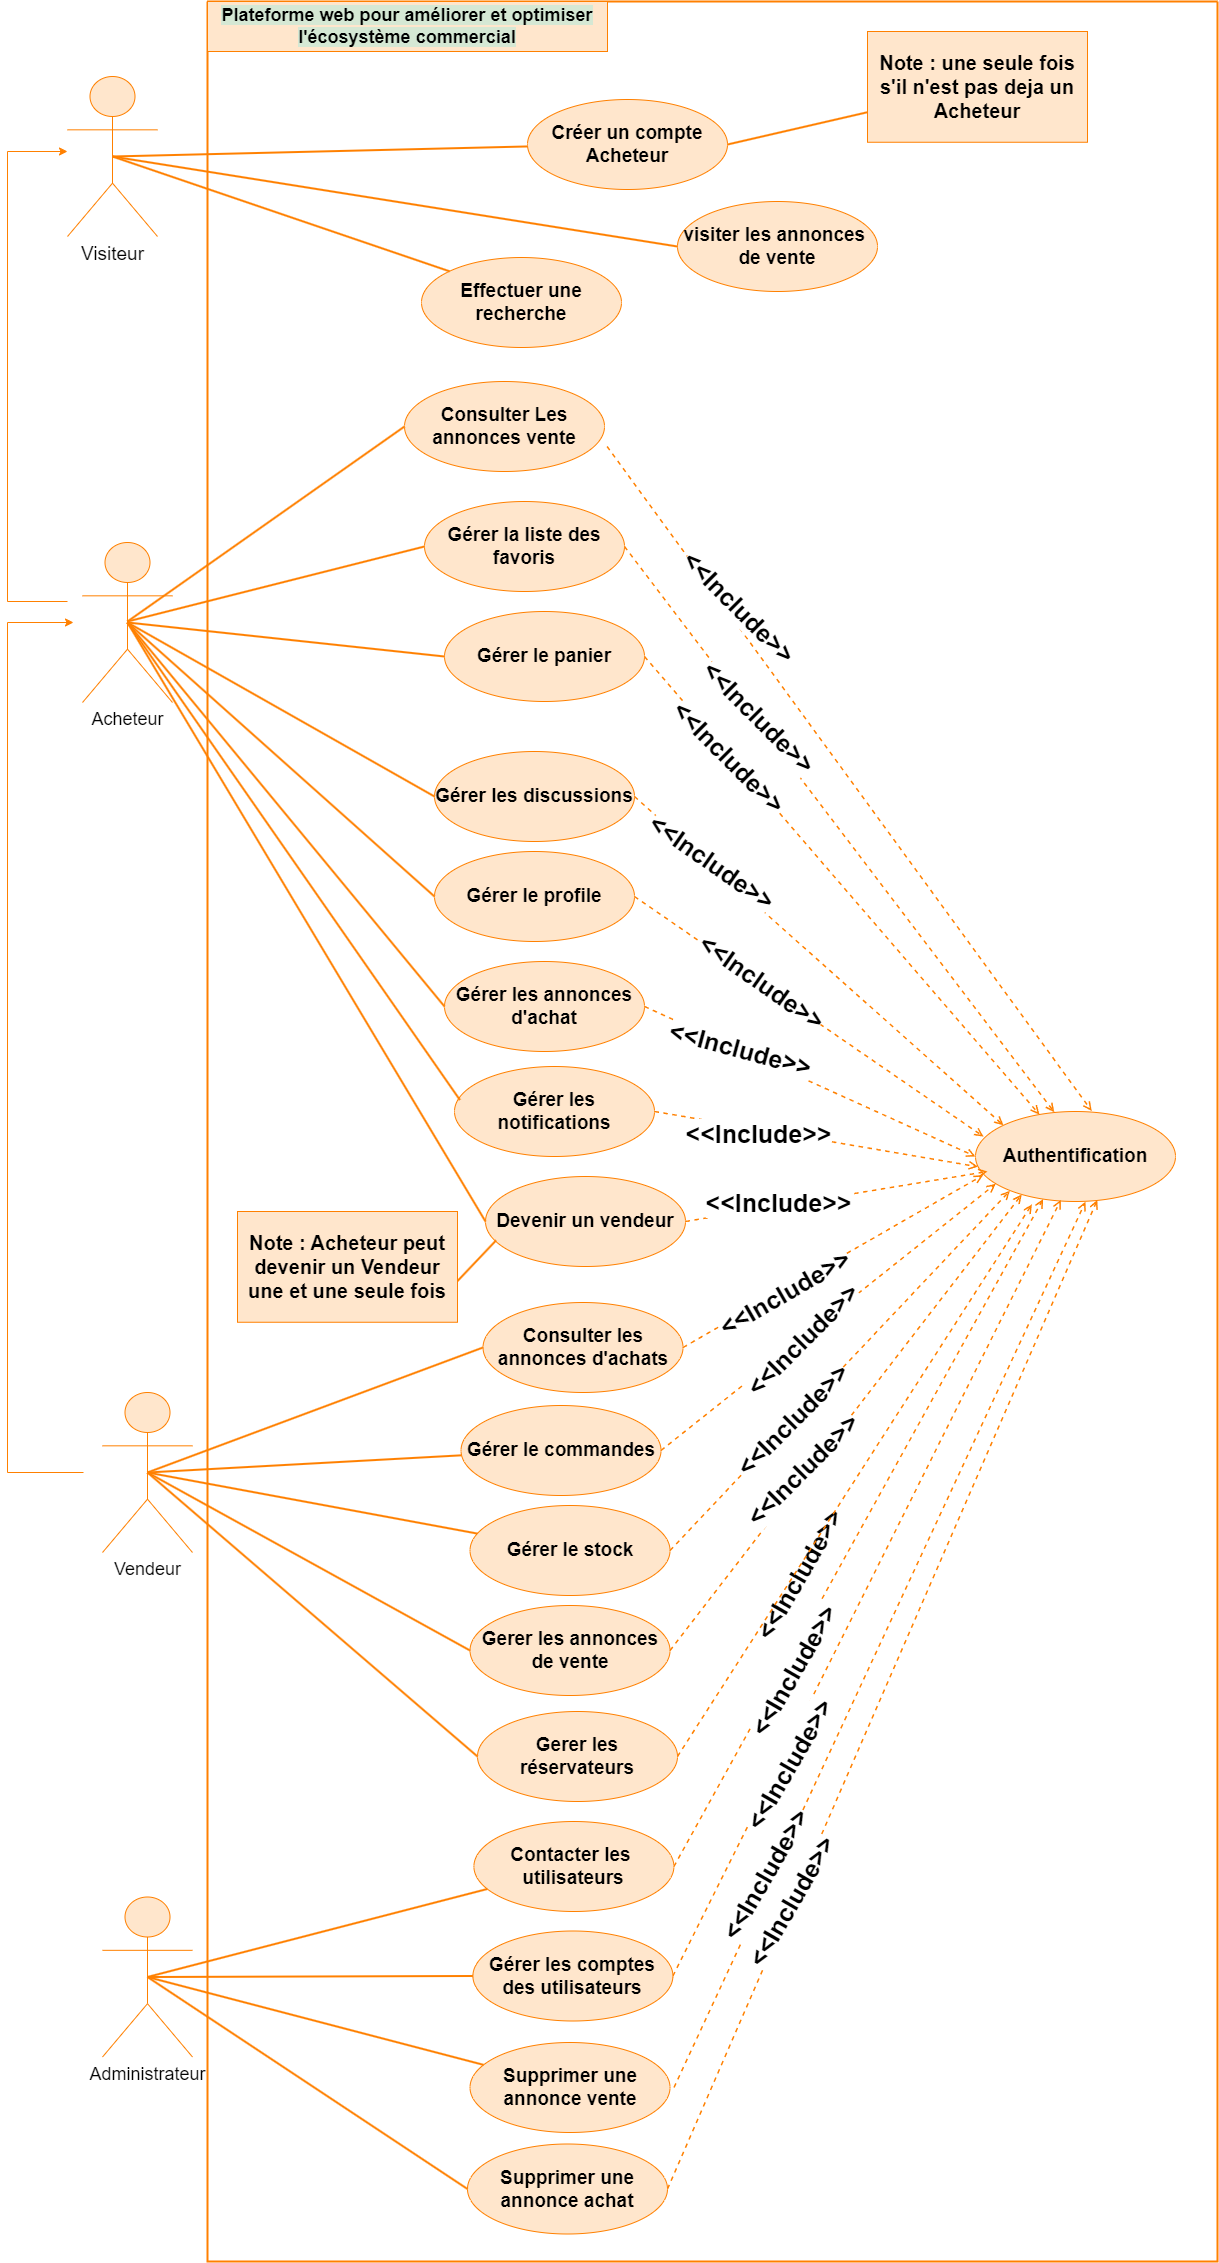
\includegraphics[width=0.7\textwidth]{images/diagramme de cas g 1.png}
\caption{Diagramme de cas d'utilisation général}
\end{figure}
\newpage
\subsubsection{Diagramme de cas d'utilisation détaillé "visiteur" }
\begin{figure}[h!]\label{fig:Diagramme de cas d'utilisation détaillé "visiteur"}
\centering
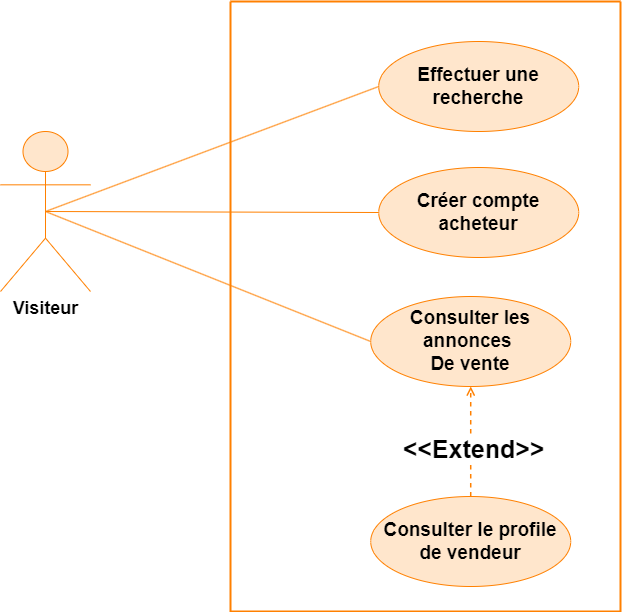
\includegraphics[width=0.5\textwidth]{images/diagramme de cas v1.png}
\caption{Diagramme de cas d'utilisation détaillé "visiteur"}
\end{figure}
\subsubsection{Diagramme de cas d'utilisation détaillé "administrateur" }
\begin{figure}[h!]\label{fig:Diagramme de cas d'utilisation détaillé "administrateur"n}
\centering
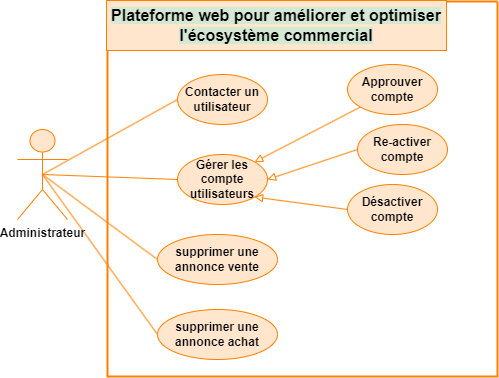
\includegraphics[width=0.6\textwidth]{images/diagramme de cas a1.png}
\caption{Diagramme de cas d'utilisation détaillé "administrateur"}
\end{figure}
\newpage
\subsubsection{Diagramme de cas d'utilisation détaillé "acheteur" }
\begin{figure}[h!]\label{fig:Diagramme de cas d'utilisation détaillé "acheteur"}
\centering
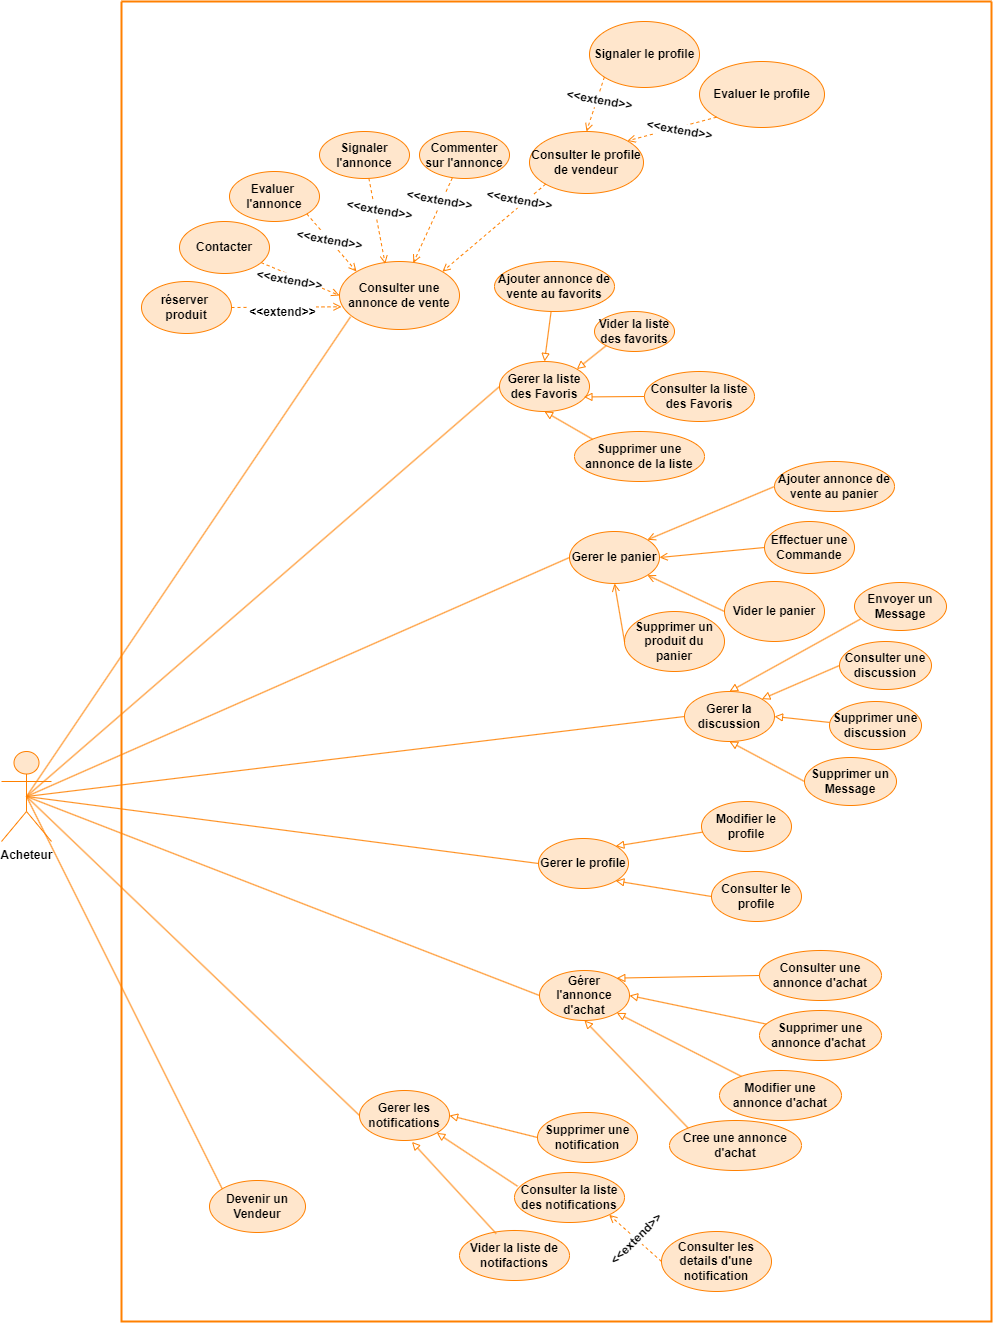
\includegraphics[width=0.9\textwidth]{images/diagramme de cas ach.png}
\caption{Diagramme de cas d'utilisation détaillé "acheteur"}
\end{figure}
\newpage
\subsubsection{Diagramme de cas d'utilisation détaillé "vendeur" }
\begin{figure}[h!]\label{fig:Diagramme de cas d'utilisation détaillé "vendeur"}
\centering
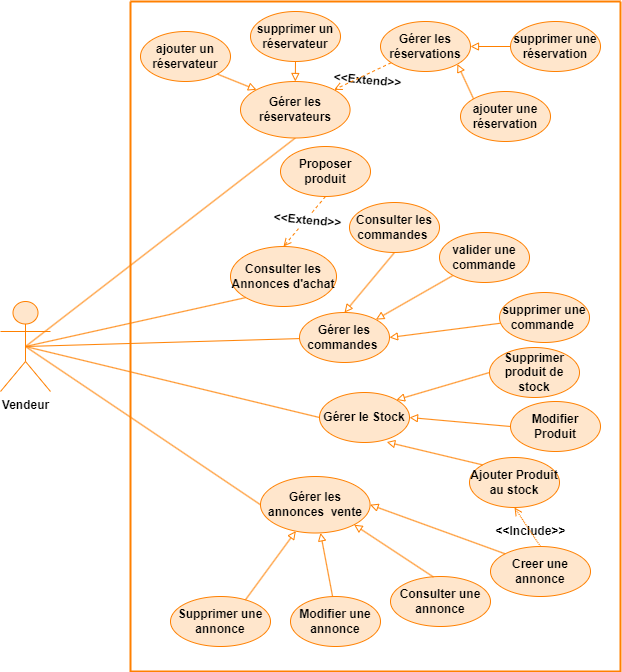
\includegraphics[width=0.5\textwidth]{images/diagramme de cas ven.png}
\caption{Diagramme de cas d'utilisation détaillé "vendeur"}
\end{figure}
\newpage
\section{Diagrammes de séquences}
\subsection{Définition}
Le diagramme de séquence permet de préciser les interactions entre l'acteur et le système avec des messages présentés dans un ordre chronologique 
\cite{séquences}
\newline Dans ce qui suit, nous allons présenter quelques exemples de diagrammes de séquence pour des cas d'utilisation importants.
\subsubsection{Cas d'utilisation "créer un compte"}
\begin{table}[h!]
    \centering
    \begin{tabular}{|c|m{10cm}|}
    \hline
         \multicolumn{2}{|c|}{Identification du cas d'utilisation "créer un compte" }\\
         \hline
         Acteur & visiteur\\
         \hline
         Pré-condition & // \\
         \hline
          & 1- L’utilisateur demande la création de compte.\\
          & 2- le système affiche le formulaire de création de compte. \\
         Scénario & 3- L’utilisateur remplit le formulaire et valide ses informations.  \\
         nominal& 4- Le système vérifie la validité des informations saisies.\\
          & 5- Le système crée un compte pour l’utilisateur.\\
          & 6- Le système envoie un email de vérification. \\
          & 7- Le système affiche la page d’authentification \\
         \hline
         Alternative  & A l’étape 4, si un champ d’information n’est pas valide ou
         l’utilisateur existe déjà, le système affiche un message d’erreur.\\
         \hline
         Post condition& Le système affiche la page d’authentification.  \\
         \hline
    \end{tabular}
    \caption{Description textuelle du cas d'utilisation "créer un compte" }
    \label{tab:cas1}
\end{table}
\begin{figure}[h!]\label{fig:Diagramme cas1}
\centering
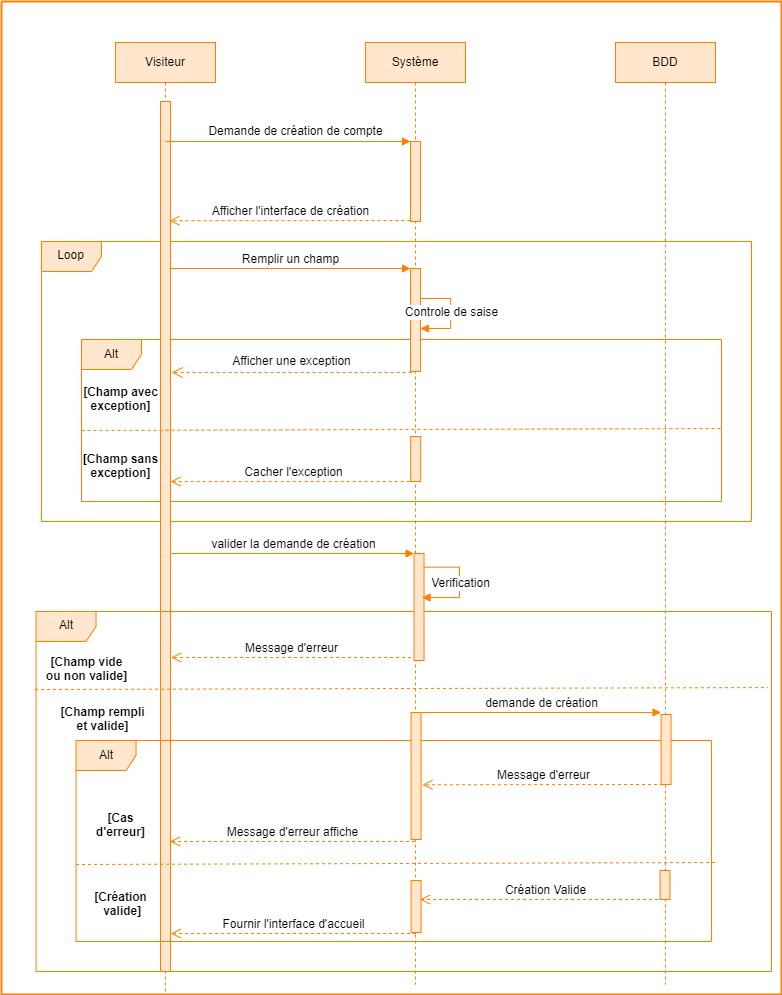
\includegraphics[width=0.8\textwidth]{images/creation de compte.png}
\caption{Diagramme de séquence du cas d'utilisation "créer un compte"}
\end{figure}


\clearpage
\subsubsection{Cas d'utilisation "authentification"}
\begin{table}[h!]
    \centering
    \begin{tabular}{|c|m{10cm}|}
    \hline
         \multicolumn{2}{|c|}{Identification dCas d'utilisation d'utilisation "authentification" }\\
         \hline
         Acteur & tous les acteurs de l’application\\
         \hline
         Pré-condition &  l’utilisateur doit être enregistré dans le système.\\
         \hline
          & 1- l'utilisateur entrer la page d'authentification\\
          & 2- le système affiche le formulaire d'authentification \\
          Scénario& 3- l'utilisateur entrer email et mot de passe \\
          nominal & 4- Le système envoie une requête à la BDD qui vérifie la correspondance entre l’email et mot de passe . \\
          & 5- La BDD confirme la correspondance correcte et retourne le rôle de l’utilisateur \\
          & 6- Le système affiche la page d’accueil.\\
         \hline
         Alternative  & A l’étape 5, si la BDD ne trouve pas de correspondance entre l’email et mot de passe le système affiche un message d’erreur.\\
         \hline
         Post condition & le système affiche la page d’accueil. \\
         \hline
    \end{tabular}
    \caption{Description textuelle du cas d'utilisation "authentification" }
    \label{tab:cas2}
\end{table}
\begin{figure}[h!]\label{fig:Diagramme cas2}
\centering
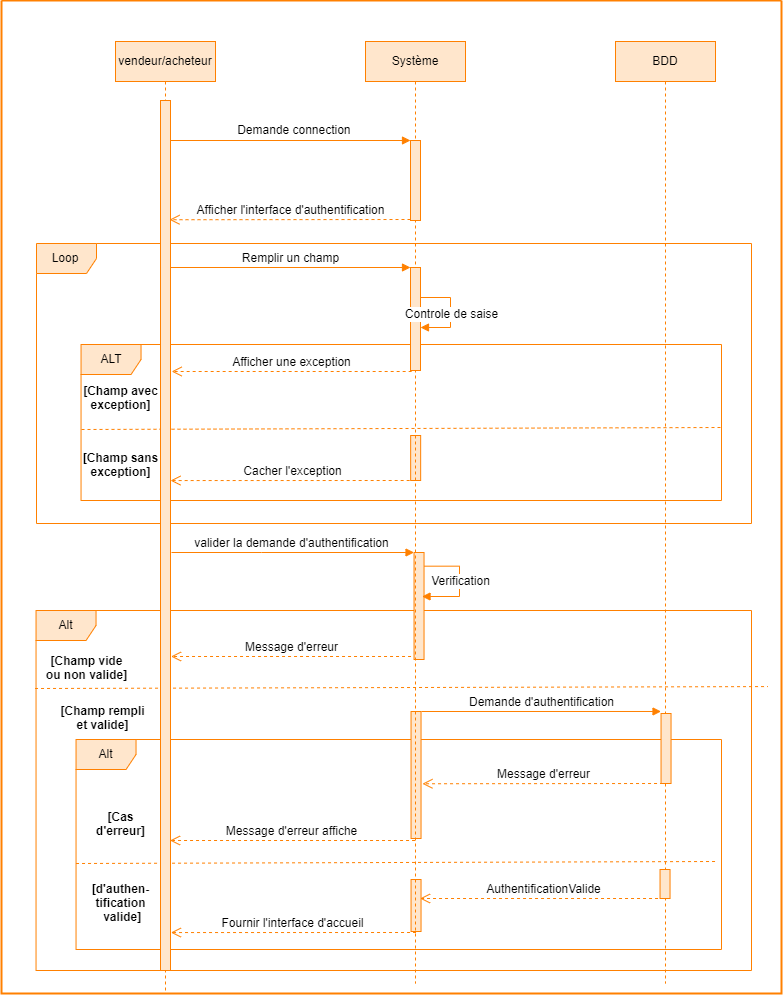
\includegraphics[width=0.8\textwidth]{images/authentifier.png}
\caption{Diagramme de séquence du cas d'utilisation "authentification"}
\end{figure}

\clearpage
\subsubsection{Cas d'utilisation "devenir un vendeur"}
\begin{table}[h!]
    \centering
    \begin{tabular}{|c|m{10cm}|}
    \hline
         \multicolumn{2}{|c|}{Identification du cas d'utilisation "devenir un vendeur" }\\
         \hline
         Acteur & acheteur\\
         \hline
         Pré-condition & L’utilisateur doit pas être déjà un vendeur\\
         \hline
          & 1- l'utilisateur demande la page "devenir un vendeur"\\
          & 2- le système affiche le formulaire correspondant\\
         Scénario&3- l'utilisateur remplit ses informations \\
         nominal& 4- le système vérifie la validité des informations saisies \\
          & 5- Le système envoie la demande à la BDD \\
          & 6- Le système affiche un message de succès\\
         \hline
         Alternative  & A l’étape 4 si un champ d’information n’est pas valide, le
         système affiche un message d’erreur.\\
         \hline
         Post condition & La demande a été envoyée avec succès. \\
         \hline
    \end{tabular}
    \caption{Description textuelle du cas d'utilisation "devenir un vendeur" }
    \label{tab:cas 3}
\end{table}
\begin{figure}[h!]\label{fig:Diagramme cas 3}
\centering
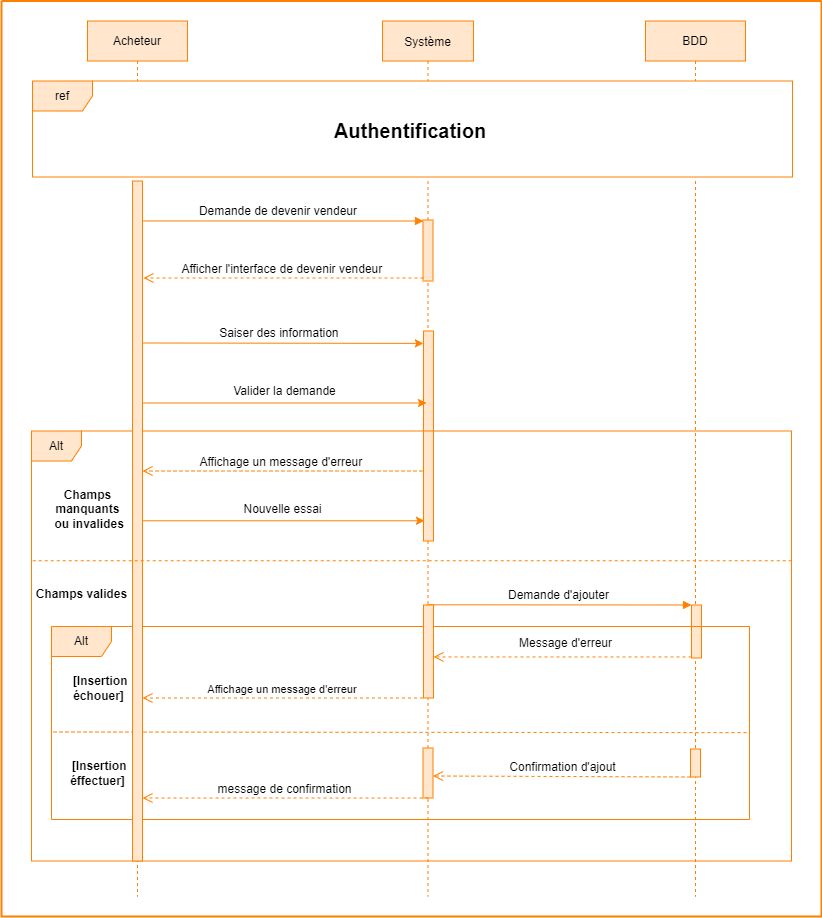
\includegraphics[width=0.8\textwidth]{images/devenir vendeur.png}
\caption{Diagramme de séquence du cas d'utilisation "devenir un vendeur"}
\end{figure}

\clearpage
\subsubsection{Cas d'utilisation "ajouter produit"}
\begin{table}[h!]
    \centering
    \begin{tabular}{|c|m{10cm}|}
    \hline
         \multicolumn{2}{|c|}{Identification du cas d'utilisation "ajouter produit" }\\
         \hline
         Acteur & vendeur\\
         \hline
         Pré-condition & L'utilisateur doit être authentifié en tant que vendeur. \\
         \hline
          & 1- l'utilisateur demande la page profile\\
          & 2- le système affiche le profile\\
          & 3- l'utilisateur demande la page de stock\\
          Scénario& 4- le système affiche le stock\\
          nominal& 5- l'utilisateur demande l’ajout d’un nouveaux produit.\\
          & 6- le système affiche le formulaire pour ajouter un produit \\
          & 7- l'utilisateur remplit le formulaire et valide les informations du produit \\
          & 8- le système vérifie la validité des informations saisies\\
          & 9- Le système affiche un message de succès, ainsi il ajoute une
          nouvelle annonce.\\
         \hline
         Alternative  & A l’étape 8 si un champ d’information n’est pas valide,  \\
         & le système affiche un message d’erreur.\\
         \hline
         Post condition& L’ajout de produit avec succès \\
         \hline
    \end{tabular}
    \caption{Description textuelle du cas d'utilisation "ajouter produit" }
    \label{tab:cas 5}
\end{table}
\begin{figure}[h!]\label{fig:Diagramme cas 5}
\centering
\includegraphics[width=0.8\textwidth]{images/Ajouter produits.png}
\caption{Diagramme de séquence du cas d'utilisation "ajouter produit"}
\end{figure}
\clearpage
\subsubsection{Cas d'utilisation "ajouter une annonce achat ou vente"}
\begin{table}[h!]
    \centering
    \begin{tabular}{|c|m{10cm}|}
    \hline
         \multicolumn{2}{|c|}{Identification du cas d'utilisation "ajouter une annonce achat ou vente" }\\
         \hline
         Acteur & Acheteur - Vendeur \\
         \hline
         Pré-condition & l’utilisateur doit être authentifié en tant que acheteur ou vendeur \\
         \hline
          & 1- l'utilisateur demande la page profile\\
          & 2- le système affiche le profile\\
          & 3- l'utilisateur demande la liste des annonces\\
          Scénario& 4- le système affiche la liste des annonces\\
          nominal& 5- L’utilisateur demande l’ajout d’une nouvelle annonce. \\
          & 6- Le système affiche le formulaire pour ajouter une annonce.\\
          & 7- L’utilisateur remplit les informations de l’annonce. \\
          & 8- Le système vérifie la validité des informations saisies. \\
       & 9- Le système affiche un message de succès, ainsi il ajoute une
          nouvelle annonce. \\
         \hline
         Alternative  & A l’étape 8 si un champ d’information n’est pas valide, le
         système affiche un message d’erreur.\\
         \hline
         Post condition & L’ajout de l’annonce avec succès \\
         \hline
    \end{tabular}
    \caption{Dscription textuelle du cas d'utilisation "ajouter une annonce achat ou vente" }
    \label{tab:cas 6}
\end{table}
\begin{figure}[h!]\label{fig:Diagramme cas 6}
\centering
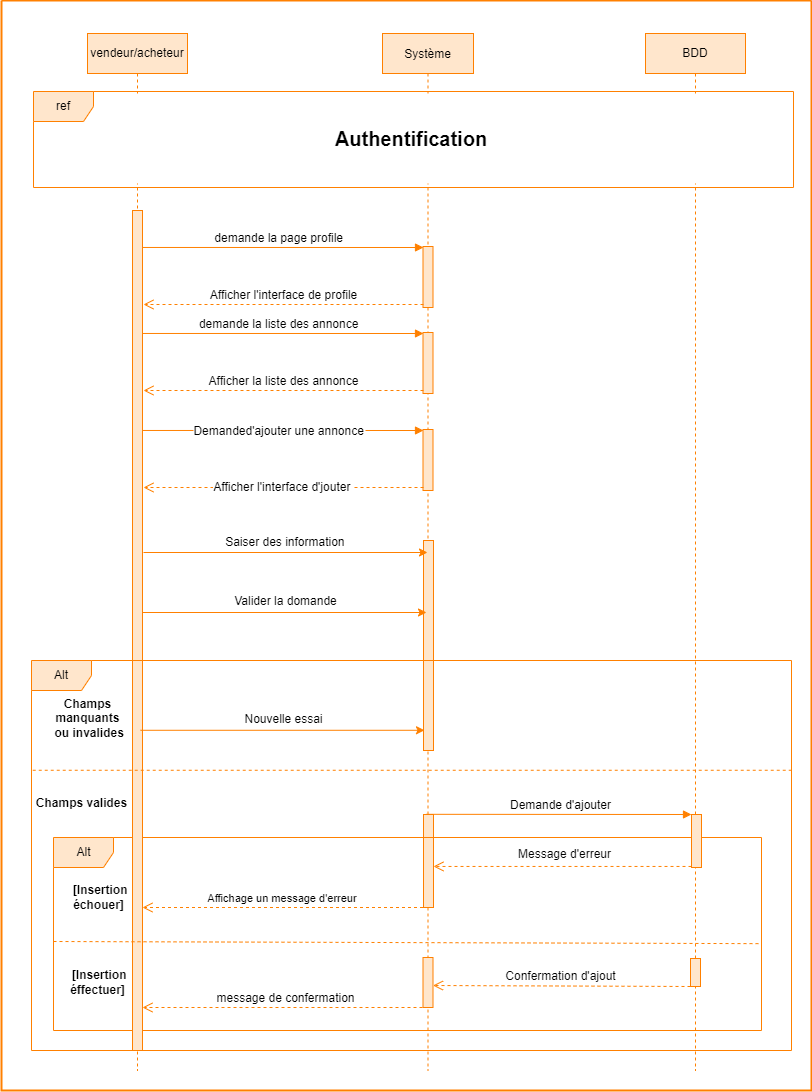
\includegraphics[width=1\textwidth]{images/ajouter annonce.png}
\caption{Diagramme de séquence du cas d'utilisation "ajouter une annonce achat ou vente"}
\end{figure}

\clearpage
\subsubsection{Cas d'utilisation "modifier une annonce achat ou vente"}
\begin{table}[h!]
    \centering
    \begin{tabular}{|c|m{10cm}|}
    \hline
         \multicolumn{2}{|c|}{Identification du cas d'utilisation "modifier une annonce achat ou vente" }\\
         \hline
         Acteur & Acheteur - Vendeur\\
         \hline
         Pré-condition & L’annonce doit être déjà existante dans la base de données, et l'utilisateur doit être authentifié en tant que acheteur ou vendeur \\
         \hline
          & 1- l'utilisateur demande la page profile\\
          & 2- le système affiche le profile\\
          & 3- l'utilisateur demande la liste des annonces\\
          Scénario& 4- le système affiche la liste des annonces\\
          nominal& 5- L’utilisateur demande la modification de l’annonce. \\
          & 6- L’utilisateur remplit les informations de l’annonce qu’il souhaite modifier, puis il valide.\\
          & 7- Le système vérifie la validité des informations saisies.\\
          & 8- Le système affiche un message de succès, ainsi il affiche les nouvelles modifications de l’annonce.\\
         \hline
         Alternative  & A l’étape 7 Si un champ d’information n’est pas valide, le
         système affiche un message d’erreur. \\
         \hline
         Post condition &  L'annonce a été modifiée avec succès.\\
         \hline
    \end{tabular}
    \caption{Description textuelle de cas d'utilisation "modifier une annonce achat ou vente" }
    \label{tab:cas 7}
\end{table}
\begin{figure}[h!]\label{fig:Diagramme cas 7}
\centering
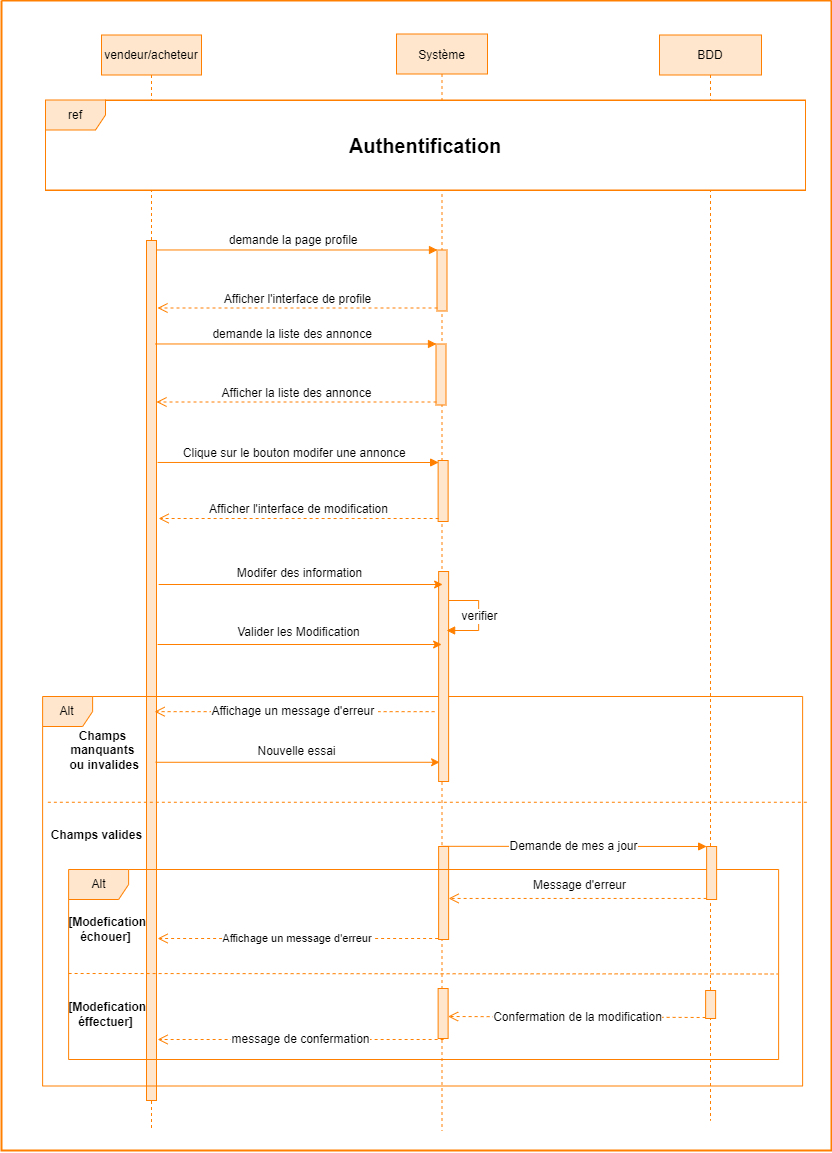
\includegraphics[width=0.8\textwidth]{images/moddifier annonce.png}
\caption{Diagramme de séquence du cas d'utilisation "modifier une annonce achat ou vente"}
\end{figure}

\clearpage
\subsubsection{Cas d'utilisation "consulter annonce vente"}
\begin{table}[h!]
    \centering
    \begin{tabular}{|c|m{10cm}|}
    \hline
         \multicolumn{2}{|c|}{Identification du cas d'utilisation "consulter annonce vente" }\\
         \hline
         Acteur & Acheteur - visiteur - vendeur\\
         \hline
         Pré-condition & L’annonce doit être déjà existante dans la base de données\\
         \hline
          & - L'utilisateur sélectionne la catégorie.\\
          Scénario& 2- Le système affiche toutes les annonces de la catégorie.\\
          nominal& 3- l'utilisateur choisir une annonce.\\
          & 4- le système afficher les details de l'annonce.\\
         \hline
         Alternative  & // \\
         \hline
         Post condition &  L’affichage les details de la annonce.\\
         \hline
    \end{tabular}
    \caption{Description textuelle du cas d'utilisation "consulter annonce vente" }
    \label{tab:cas 7c}
\end{table}
\begin{figure}[h!]\label{fig:Diagramme cas 7c}
\centering
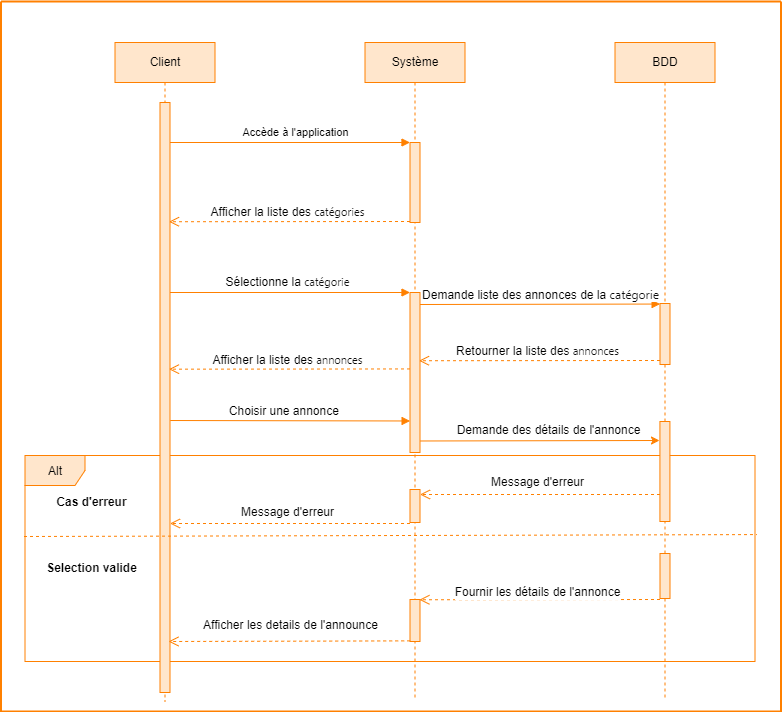
\includegraphics[width=0.8\textwidth]{images/consulter une annonce.png}
\caption{Diagramme de séquence du cas d'utilisation "consulter annonce vente"}
\end{figure}

\clearpage
\subsubsection{Cas d'utilisation "ajouter au panier"}
\begin{table}[h!]
    \centering
    \begin{tabular}{|c|m{10cm}|}
         \hline
         \multicolumn{2}{|c|}{Identification du cas d'utilisation "ajouter au panier" }\\
         \hline
         Acteur & acheteur\\
         \hline
         Pré-condition & L'utilisateur doit être authentifié en tant que acheteur. \\ 
         \hline
         Scénario& 1- l'utilisateur consulte une annonce\\
          nominal& 2- l'utilisateur demande l’ajout d’une annonce au panier.\\
          & 3- Le système ajoute l'annonce au panier. \\
         \hline
         Alternative  & vérification de quantité\\
         \hline
         Post condition& L’ajout de l'annonce avec succès \\
         \hline
    \end{tabular}
    \caption{Description textuelle de cas d'utilisation "ajouter au panier" }
    \label{tab:cas 9}
\end{table}
\begin{figure}[h!]\label{fig:Diagramme cas 9} 
\centering
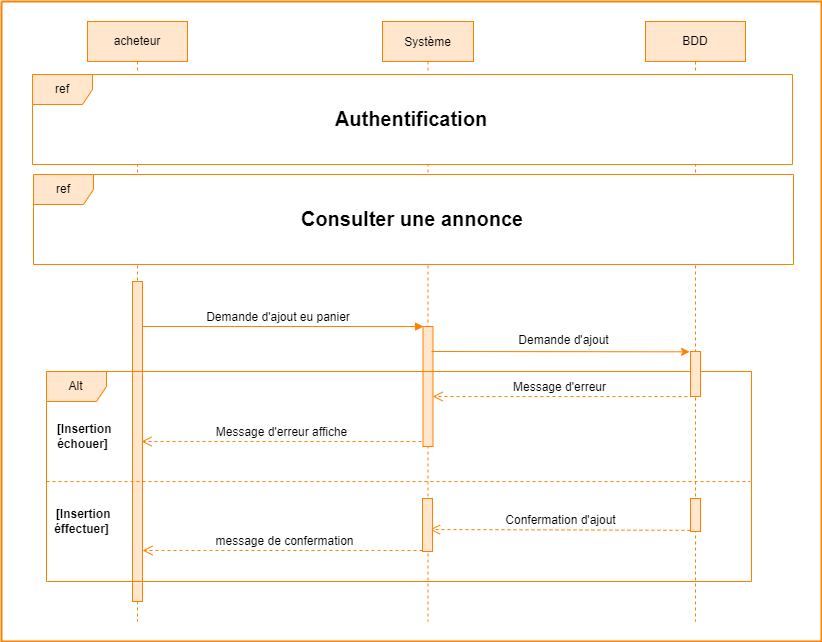
\includegraphics[width=0.8\textwidth]{images/Ajouter au panier.png}
\caption{Diagramme de séquence du cas d'utilisation "ajouter au panier"}
\end{figure}

\clearpage
\subsubsection{Cas d'utilisation "effectuer une commande"}
\begin{table}[h!]
    \centering
    \begin{tabular}{|c|m{10cm}|}
        \hline
        \multicolumn{2}{|c|}{Identification du cas d'utilisation "effectuer une commande"}\\
        \hline
        Acteur & acheteur\\
        \hline
        Pré-condition &l'utilisateur doit être authentifié en tant que acheteur,et un produit au minimum dans le panier \\ 
        \hline
         & 1- l'utilisateur demande la page panier.\\
         Scénario& 2- le systéme affiche la page panier.\\
         nominal& 3- l'utilisateur sélectionner des produit.\\
         & 4- L'utilisateur effectuer une commande.\\
        \hline
        Alternative  &quantité indisponible\\
        \hline
        Post condition& La commande a été ajoutée avec succès. \\
        \hline
    \end{tabular}
    \caption{Description textuelle de cas d'utilisation "effectuer une commande" }
    \label{tab:cas 8}
\end{table}
\begin{figure}[h!]\label{fig:Diagramme cas 8}
\centering
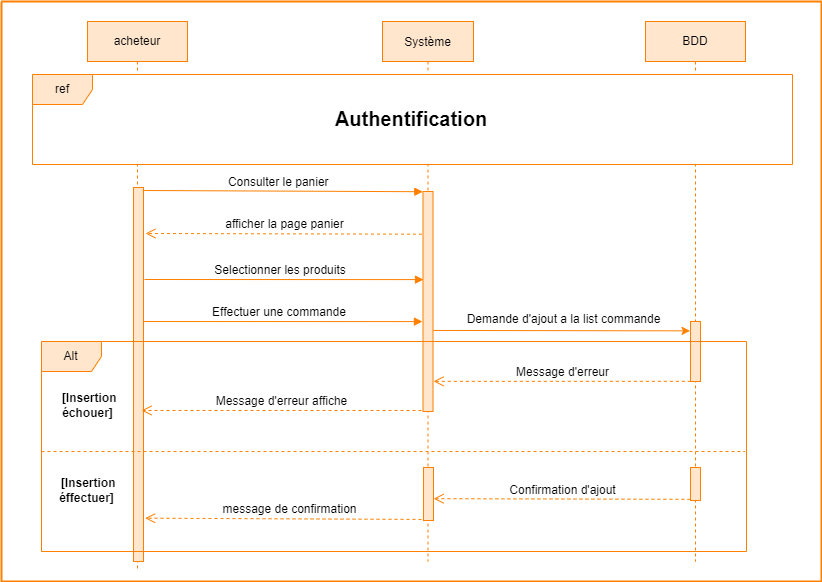
\includegraphics[width=0.8\textwidth]{images/Effectuer une commande.png}
\caption{Diagramme de séquence du cas d'utilisation "effectuer une commande"}
\end{figure}


\clearpage
\subsubsection{Cas d'utilisation "valider compte vendeur"}
\begin{table}[h!]
    \centering
    \begin{tabular}{|c|m{10cm}|}
    \hline
         \multicolumn{2}{|c|}{Identification du cas d'utilisation "valider compte vendeur" }\\
         \hline
         Acteur & administrateur\\
         \hline
         Pré-condition &  L'utilisateur doit être authentifié en tant que administrateur.\\
         \hline
          & 1- l'administrateur demande la Liste des demandes\\
          & 2- le système afficher la liste des demandes\\
          & 3- L'administrateur sélectionne la demande en question. \\
          & 4- Le système affiche les détails du vendeur.\\
          Scénario & 5- L'administrateur valide la demande du vendeur. \\
          nominal& 6- Le système affiche un message de confirmation.\\
          & 7- L'administrateur confirme la validation.\\
          & 8- Le système affiche un message de succès et retire la demande de la liste des demandes.\\
         \hline
         Alternative  & À l'étape 7, si l'administrateur annule la validation, la demande ne sera pas validée. \\
         \hline
         Post condition & La demande a été validée avec succès. \\
         \hline
    \end{tabular}
    \caption{Description textuelle du cas d'utilisation "valider compte vendeur" }
    \label{tab:cas 12}
\end{table}
\begin{figure}[h!]\label{fig:Diagramme cas 12}
\centering
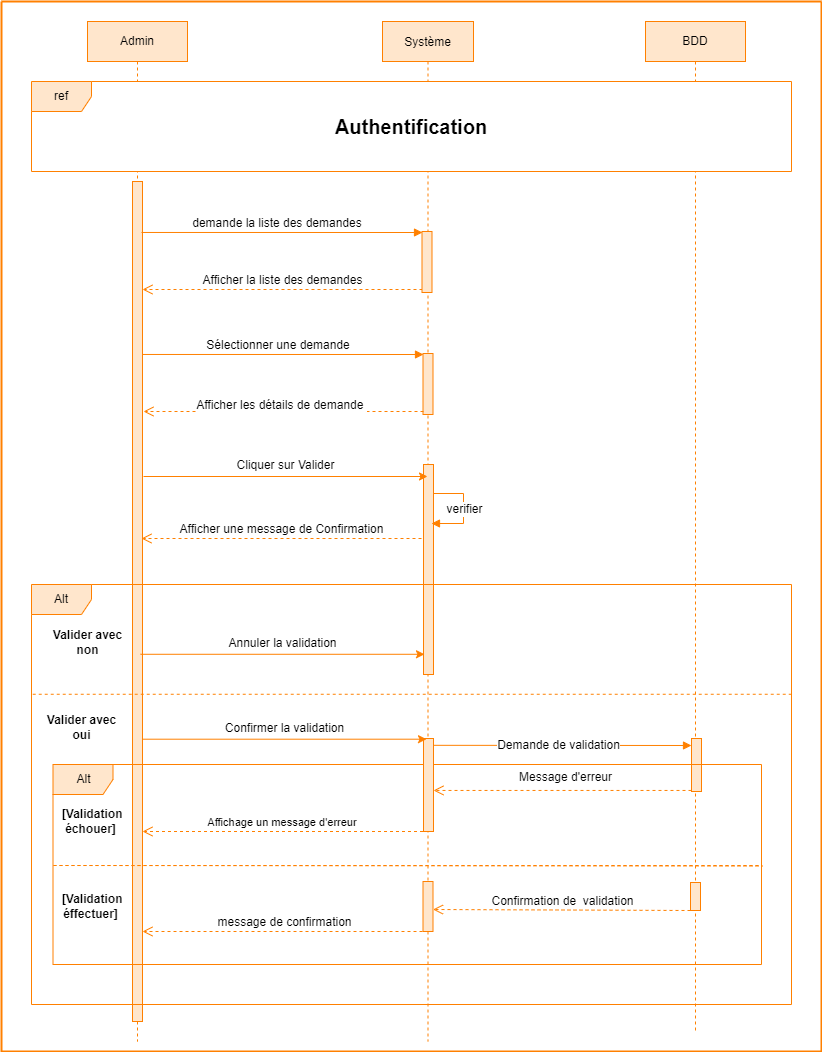
\includegraphics[width=0.8\textwidth]{images/valider compte vendeur.png}
\caption{Diagramme de séquence du cas d'utilisation "valider compte vendeur"}
\end{figure}
\clearpage
\section{Conclusion}
Ce chapitre a permis de définir clairement les besoins spécifiques pour la création d'une plateforme web et d'une application mobile. Les diagrammes de cas d'utilisation et de séquence ont illustré les interactions entre les utilisateurs et le système, facilitant ainsi la compréhension des exigences fonctionnelles. Cette démarche a établi une base solide pour le développement, en assurant que toutes les fonctionnalités nécessaires soient bien identifiées et documentées.
%=======================================================
\chapter{Analyse des besoins}
\section{Introduction}
Après avoir exprimé les besoins, il est crucial d'analyser ces exigences en détail pour assurer une compréhension approfondie et pour identifier les éventuelles lacunes ou conflits. Ce chapitre se consacre à cette analyse, en détaillant les processus métier et les flux de travail à l'aide de diagrammes de séquence détaillés et de diagrammes d'activité. Cette étape permet de décomposer les besoins en éléments plus petits et plus gérables, de vérifier leur faisabilité et de préparer des solutions optimisées. L'analyse approfondie garantit que toutes les exigences sont bien comprises et alignées avec les objectifs du projet.
\section{Les diagrammes de séquence détaillés}
\subsection{Définition}

Les diagrammes de séquence détaillés sont un type de diagramme UML utilisé pour modéliser les interactions entre différentes entités d'un système au fil du temps. Ils montrent les échanges de messages entre les participants (objets ou acteurs), représentés par des lignes de vie. Les messages sont illustrés par des flèches horizontales qui indiquent la direction de l'interaction.
\newline
\phantom{h}
\newline
Les diagrammes de séquence détaillés se concentrent sur l'ordre chronologique des interactions et peuvent inclure des opérations spécifiques, des conditions d'exécution, des boucles, des options et des alternatives pour montrer comment les entités collaborent. Ils sont utiles pour comprendre et communiquer la dynamique d'un système de manière précise et visuelle.
\cite{séquenced}
\subsection{La différence entre un diagramme de séquence simple et détaillé.}

Les diagrammes de séquence sont un type de diagramme UML utilisé pour représenter les interactions entre des objets ou acteurs dans un système au fil du temps.
\newline
\phantom{h}
\newline
La principale différence entre un diagramme de séquence simple et un diagramme de séquence détaillé réside dans le niveau de détail et de complexité des interactions modélisées :
\begin{itemize}
    \item \textbf{Diagramme de séquence simple:}Il montre des interactions de base entre les acteurs ou objets, avec des messages et des lignes de vie. Ces diagrammes sont généralement courts et faciles à comprendre, adaptés pour illustrer des scénarios de haut niveau ou simples.
    \item \textbf{Diagramme de séquence détaillé:}Il inclut un niveau de détail plus élevé, montrant des interactions complexes avec des conditions d'exécution, des boucles, des options (\textbf{opt}) et des alternatives (\textbf{alt}). Il reflète plus précisément les communications et les flux de contrôle dans le système, et convient à la modélisation de scénarios spécifiques et complexes.
\end{itemize}
Dans ce qui suit, nous allons présenter les diagrammes de séquence détaillés pour quelques cas d'utilisation.

\subsubsection{Cas d'utilisation "authentification détaillé"}
\begin{figure}[h!]\label{fig:Diagramme cas 1d}
\centering
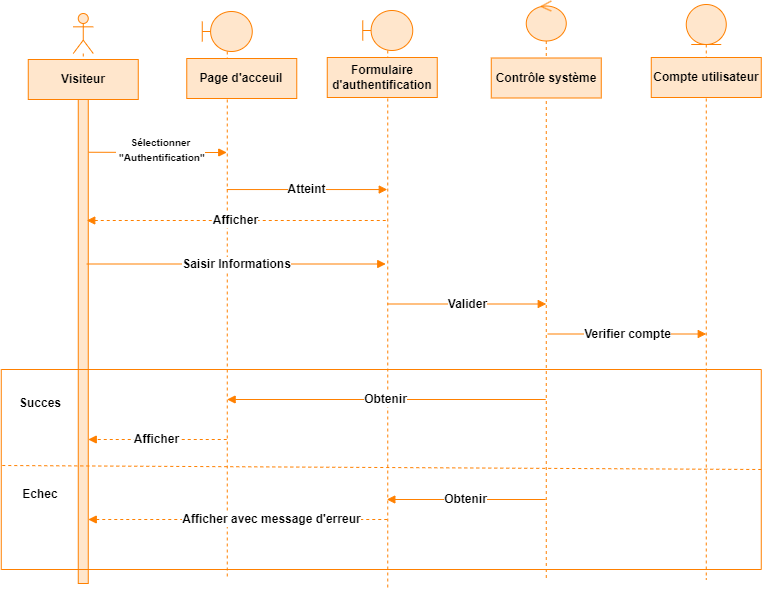
\includegraphics[width=0.8\textwidth]{images/Authentification d.png}
\caption{Diagramme de séquence du cas d'utilisation "authentification détaillé"}
\end{figure}



\newpage
\subsubsection{Cas d'utilisation "devenir un grossiste détaillé"}
\begin{figure}[h!]\label{fig:Diagramme cas 2d}
\centering
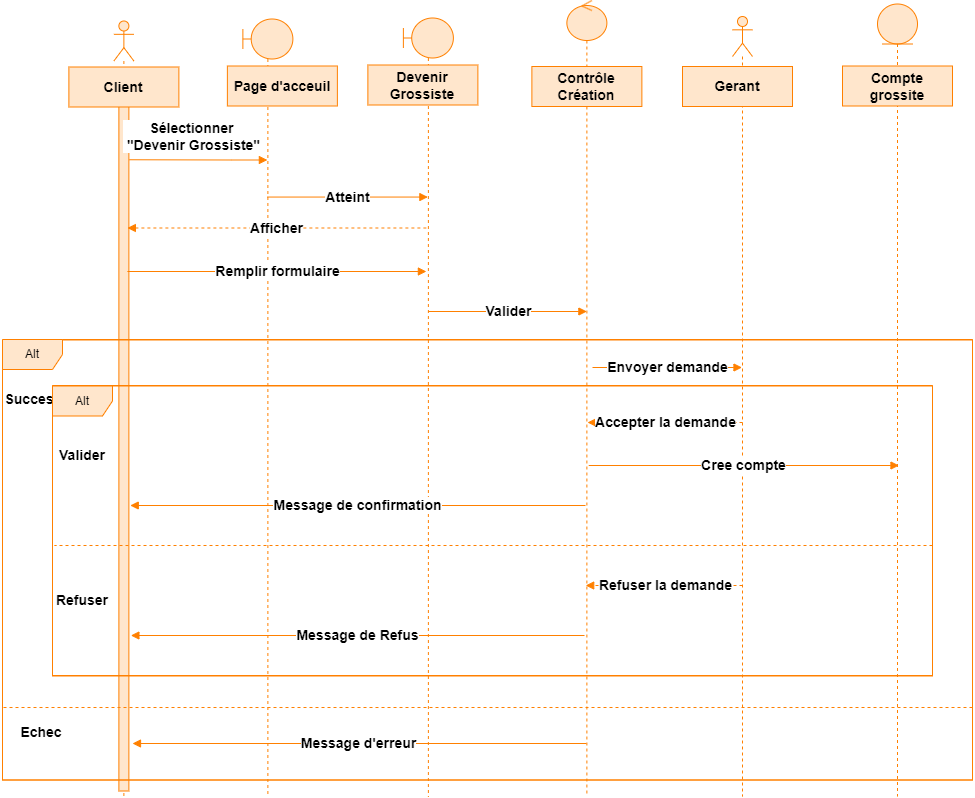
\includegraphics[width=0.8\textwidth]{images/Devenir un grossiste d.png}
\caption{Diagramme de séquence du cas d'utilisation "devenir un grossiste détaillé"}
\end{figure}

\newpage
\subsubsection{Cas d'utilisation "ajouter une annonce détaillé"}
\begin{figure}[h!]\label{fig:Diagramme cas 3d}
\centering
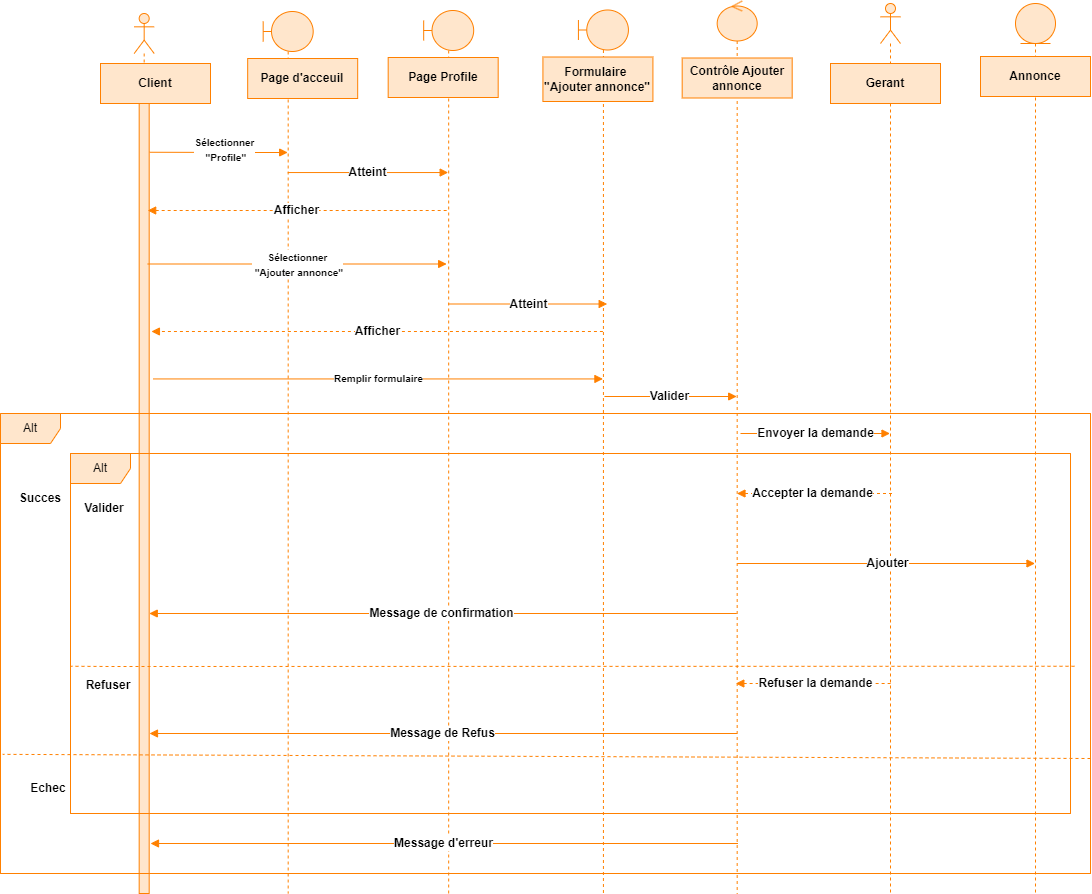
\includegraphics[width=0.8\textwidth]{images/Ajouter une annonce d.png}
\caption{Diagramme de séquence du cas d'utilisation "ajouter une annonce détaillé"}
\end{figure}

\newpage
\subsubsection{Cas d'utilisation "effectuer une commande détaillé"}
\begin{figure}[h!]\label{fig:Diagramme cas 4d}
\centering
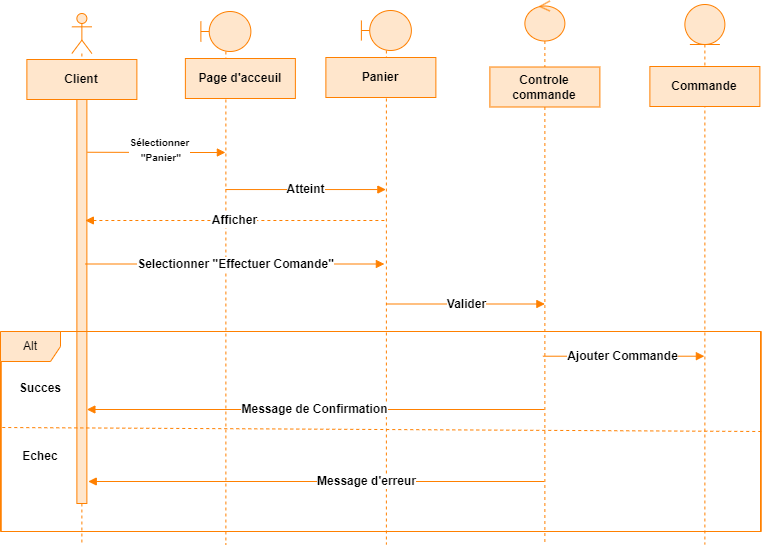
\includegraphics[width=0.8\textwidth]{images/Effectuer une commande d.png}
\caption{Diagramme de séquence du cas d'utilisation "effectuer une commande détaillé"}
\end{figure}


\newpage
\subsubsection{Cas d'utilisation "contacter détaillé"}
\begin{figure}[h!]\label{fig:Diagramme cas 5d}
\centering
\includegraphics[width=0.8\textwidth]{images/contacter d.png}
\caption{Diagramme de séquence du cas d'utilisation "contacter détaillé"}
\end{figure}




\section{Diagramme d'activité}
\subsection{Définition}
Un diagramme d'activité représente visuellement le flux de contrôle entre les différentes activités d'un processus dans le domaine de l'ingénierie logicielle et de la gestion des processus.  d'activité est une méthode visuelle utilisée dans l'ingénierie logicielle et la gestion des processus pour représenter le flux de contrôle entre différentes activités d'un processus. Il aide à visualiser les étapes et les décisions d'un processus, que ce soit dans le cadre du développement logiciel ou de la modélisation des processus métier.
\cite{activite}
\newline Dans les sections suivantes, nous présenterons plusieurs exemples de diagrammes d'activité pour divers cas d'utilisation.
\clearpage
\subsubsection{Cas d'utilisation "créer compte"}
\begin{figure}[h!]\label{fig:activite cree}
    \centering
    \includegraphics[width=0.9\textwidth]{images/activite créer compte.png}
    \caption{Diagramme d'activité "créer compte"}
\end{figure}
\clearpage
\subsubsection{Cas d'utilisation "authentification"}
\begin{figure}[h!]\label{fig:activite auth}
    \centering
    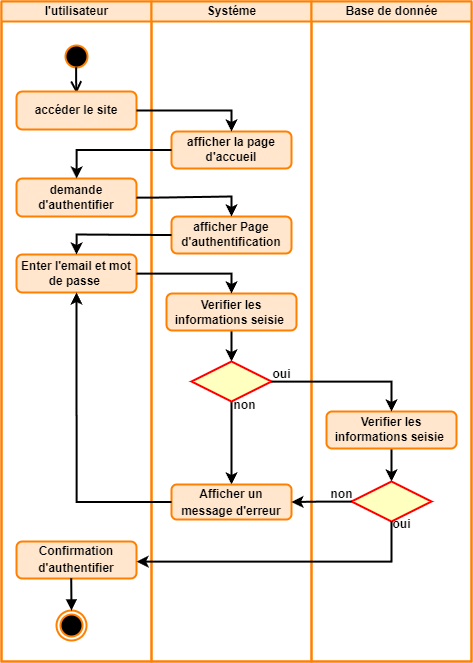
\includegraphics[width=0.9\textwidth]{images/activite Authontification.png}
    \caption{Diagramme d'activité "authentification"}
\end{figure}
\clearpage
\subsubsection{Cas d'utilisation "demande devenire vendeur"}
\begin{figure}[h!]\label{fig:activite demande}
    \centering
    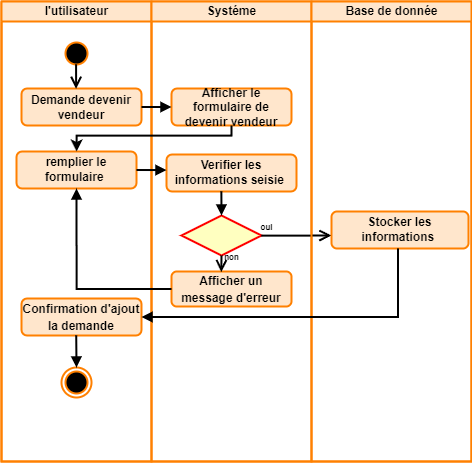
\includegraphics[width=1\textwidth]{images/activite demande devenire vender.png}
    \caption{Diagramme d'activité "demande devenire vendeur"}
\end{figure}
\clearpage
\subsubsection{Cas d'utilisation "ajouter une annonce"}
\begin{figure}[h!]\label{fig:activite ajoutera}
    \centering
    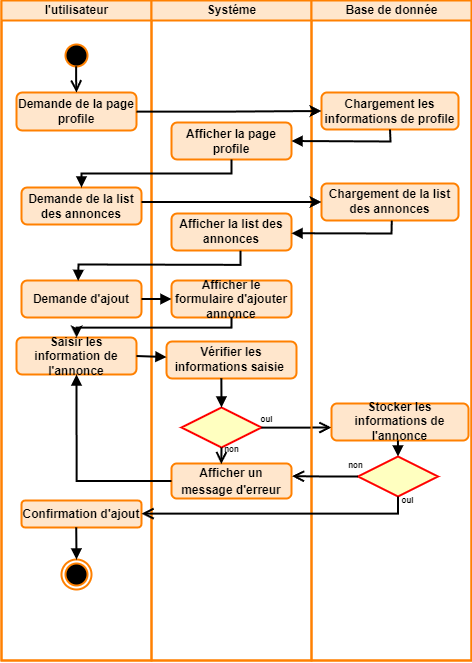
\includegraphics[width=0.9\textwidth]{images/activite Ajouter annonce.png}
    \caption{Diagramme d'activité "ajouter une annonce"}
\end{figure}
\clearpage
\subsubsection{Cas d'utilisation "effectuer une commande"}
\begin{figure}[h!]\label{fig:activite }
    \centering
    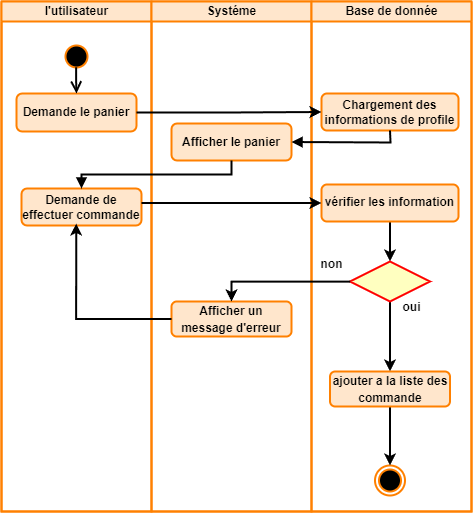
\includegraphics[width=1\textwidth]{images/activite effecter commande.png}
    \caption{Diagramme d'activité "effectuer une commande"}
\end{figure}
\section{Conclusion}
L'analyse détaillée des besoins a approfondi les spécifications initiales. Les diagrammes de séquence détaillés et d'activité ont permis de visualiser les processus métier et les flux de travail en détail. Cela a mis en lumière les interactions complexes et les dépendances, permettant d'identifier les améliorations et les optimisations nécessaires avant de passer à la phase de conception.






%=====================================>
\chapter{Conception}
\section{Introduction}
La conception est l'étape où les besoins analysés sont transformés en une architecture concrète et en un design détaillé. Ce chapitre se focalise sur l'élaboration du diagramme de classe, qui définit les structures de données, les composants du système et leurs relations. La conception structurelle est cruciale pour s'assurer que le système est modulaire, extensible et maintenable. En établissant une architecture claire, ce chapitre permet de guider les développeurs dans la mise en œuvre technique du projet, en s'assurant que chaque composant fonctionne harmonieusement dans l'ensemble du système.
\section{Diagramme de classe}
Le diagramme de classes est généralement considéré comme le plus important dans
un développement orienté objet. Il représente l’architecture conceptuelle du système : il
décrit les classes que le système utilise, ainsi que leurs liens, que ceux-ci représentent un
emboîtage conceptuel (héritage) ou une relation organique (agrégation).
\subsection{Dictionnaire de données}
Le dictionnaire des données est un document qui regroupe toutes les données que vous
aurez à conserver dans votre base. Pour chaque donnée, il indique le code mnémonique,la
désignation, le type de donnée
\newline Le tableau suivant représente le dictionnaire de données de notre système
\begin{table}[H]
    \centering
    \begin{tabular}{ | m{2,6cm} | m{3,2cm}| m{3cm} |m{0,9cm}|m{0,9cm}|l|}
    \hline
         Classe&\multicolumn{3}{c}{Attributs}&\phantom{h} &Methodes\\
         \hline &Nom&Description&Type&Taille&\\\cline{2-5}
                                        &id\_administrateur&l'id d'administrateur&AN&15& \\\cline{2-5}
                        Administrateur  &nom\_utilisateur&le nom de l'administrateur&AN&20& \\\cline{2-5}
                                        &mot\_de\_pass&le mot de pass de l'administrateur &AN&20& \\\hline

 \end{tabular}
\end{table}
\begin{table}[H]
    \centering
    \begin{tabular}{ | m{2,6cm} | m{3,2cm}| m{3cm} |m{0,9cm}|m{0,9cm}|l|}
    \hline
         Classe&\multicolumn{3}{c}{Attributs}&\phantom{h} &Methodes\\
         \hline &Nom&Description&Type&Taille&\\\cline{2-5}
                                        &id\_acheteur&l'id de acheteur&AN&15& \\\cline{2-5}
                                        &nom         &le nom de l'acheteur&A&15& \\\cline{2-5}
                                        &prenom      &le prenom de l'acheteur&A&15& \\\cline{2-6}
                                Acheteur&email       &l'email de l'acheteur&AN&30&s'authentifier() \\\cline{2-6}
                                        &num         &le numéro de l'acheteur&N&10&modifer\_profil() \\\cline{2-6}
                                        &mot\_de\_pass&le mot de pass de l'acheteur&AN&15& supprimer\_profile()\\\cline{2-6}
                                        &adresse     &l'adresse de l'acheteur&AN&30&proposer\_produit()\\\cline{2-6}
                                        &photo       &le photo de l'acheteur&image&10&\\\hline


                                        &id\_vendeur &l'id de vendeur&AN&15& \\\cline{2-6}
                                        &code\_registre \_commerce&le code de registre Commerce de vendeur&N&15&devenir\_vendeur() \\\cline{2-6}
                                Vendeur &num\_carte \_national&le numéro de carte national de vendeur&N&15&valider\_vendeur()\\\cline{2-6}
                                        &nom\_companie &le nom de companie de vendeur&AN&15&évaluer\_vendeur()\\\cline{2-6}
                                        &nombre \_Evaluations&les nombre des evaluation&N&20&signaler\_vendeur()\\\cline{2-6}
                                        &catégorie\_vendeur&le catégorie de commerce de vender&A&20& \\\cline{2-5}
                                        &bio\_vendeur&le biographie de vendeur&AN&100& \\\hline

                            Discussion  &id\_discussion&l'id de discussion&AN&15&supprimer\_discussion() \\\cline{2-6}
                                        &date\_debut&la date de debut discussion&date&8&contacter\_vendeur()\\\hline

                                        &id\_message&l'id de message&AN&15& \\\cline{2-6}
                                        &etat\_message&l'etat de message&A&10&notification\_message() \\\cline{2-6}
                              Message   &date\_envoyer&la date de envoie le message&date&8&envoyer\_message() \\\cline{2-6}
                                        &date\_vu&la date de vu de message&date&8&supprimer\_message() \\\cline{2-6}
                                        &contenu\_message&le contenu de message&AN&100& \\\hline


 \end{tabular}
\end{table}

\begin{table}[H]
    \centering
    \begin{tabular}{ | m{2,6cm} | m{3,2cm}| m{3cm} |m{0,9cm}|m{0,9cm}|l|}
    \hline
                                          &id\_commande&l'id de commande&AN&15& \\\cline{2-6}
                                          &date\_commande&la date de commande&date&8&effectuer\_commande() \\\cline{2-6}
                                Commande  &etat\_commande&l'etat de commande&A&10&valider\_commande() \\\cline{2-6}
                                          &montant\_livraison&            &A&4&annuler\_commande()\\\cline{2-6}
                                          &montant\_totale \_commande&le montant totale de la commande&N&15&notification\_Commande() \\\hline


                                          &id\_produit&l'id de produit&AN&15&ajouter\_produit() \\\cline{2-6}
                                Produit   &nom\_produit&nom de produit&A&10&modifier\_produit() \\\cline{2-6}
                                          &quantité\_produit&la quantité de produit sur le stock&N&10&supprimer\_produit()\\\cline{2-6}
                                          &                 &                                   & &  &reserver\_produit() \\\hline

                                          &id\_panier&l'id de panier&AN&15&ajouter\_au\_panier() \\\cline{2-6}
                                Panier    &montant\_totale&le montant totale de panier&N&10&modifier\_panier() \\\cline{2-6}
                                          &                 &                         & &  &supprimer\_du\_panier()\\\cline{2-6}
                                          &                 &                         & &  &vider\_le\_panier()\\\hline


                                          &titre\_annonce&le titre de l'annonce&AN&20&commenter\_annonce()\\\cline{2-6}
                                          &description&la description d'annonce&AN&100&signaler\_annonce()\\\cline{2-6}
                                Annonce   &date\_de \_publication&la date de publication&date&8&créer\_annonce()\\\cline{2-6}
                                          &quantité&le quantité de produit &N&10&Modifie \_annonce()\\\cline{2-6}
                                          &photo &la photo de l'annonce   &image&10&supprimer\_annonce()\\\cline{2-6}
                                          & &   &&&effectuer\_recherche()\\\cline{2-6}
                                          & &   &&&ajouteraufavoris()\\\cline{2-6}
                                          & &   &&&suprimerdefavoris()\\\cline{2-6}
                                          & &   &&&signaler\_annonce()\\\hline

                        Annonce \_achat   &id\_annonce \_achat &l'id de l'annonce d'achat&AN&15& \\\hline
                                  


                                          &id\_annonce\_vente&l'id d'annonce de vente&AN&15&\\\cline{2-5}
                                          &prix\_produit&le prix de produit&N&10&\\\cline{2-6}
                        Annonce \_vente   &livraison&la disponibilité de livraison&A&5&ajouteraufavoris() \\\cline{2-6}
                                          &montant\_livraison&le prix de livraison&N&10&suprimierdefavoris() \\\cline{2-6}
                                          &quantité\_min&la quantité minimal de vente&N&10& \\\hline


                                                              
          
    \end{tabular}
\end{table}



\begin{table}[H]
    \centering
    \begin{tabular}{ | m{2,6cm} | m{3,2cm}| m{3cm} |m{0,9cm}|m{0,9cm}|l|}
    \hline            
                        Evaluation \_annonce&id\_reaction&l'id de reaction&AN&15& \\\cline{2-5}
                                            &react&réagir avec j'aime ou je n'aime pas&A&5& \\\hline


                                            &contenu&le contenu de &AN&100&Notification\\
                                Commentaires&\_commentaire&commentaires &  &   &\_Commentaire()\\\cline{2-6}
                                            &date \_commentaires&la date de commentaires&date&8&\\\hline

\end{tabular}
\caption{Dictionnaire de données}
\label{tab:Dictionnaire}
\end{table}
\subsection{Les règles de gestion}
Voici les règles de gestion de notre système
\begin{enumerate}
    \item l’acheteur peut évaluer un ou plusieurs vendeurs.
    \item un acheteur peut évaluer ou commenter sur une ou plusieurs annonces de vente.
    \item un acheteur peut ajouter des annonces de vente aux favoris.
    \item un acheteur peut ajouter une ou plusieurs annonces de vente au panier.
    \item un acheteur peut effectuer une ou plusieurs commandes.
    \item un acheteur peut publier une ou plusieurs annonces d’achat.
    \item un acheteur peut signaler un vendeur ou une annonce.
    \item un acheteur a la possibilité de recevoir des notifications de messages, des commentaires sur ces annonces d’achat et des propositions des vendeurs.
    \item l’acheteur et le vendeur peuvent échanger des messages. si leurs discussion est déjà ouvert
    \item un vendeur peut publier une ou plusieurs annonces de vente.
    \item un vendeur peut ajouter des produits au stock. 
    \item un vendeur possède toutes les fonctionnalités de l'acheteur.
    \item un vendeur a la possibilité de valider ou d'annuler une commande.
    \item un vendeur a la possibilité de proposer un produit à un utilisateur à partir d'une annonce d'achat.
    \item un vendeur a la possibilité de recevoir des notifications de messages, des commentaires sur ces annonces de vente, une évaluation de compte et des commandes.
    \item un administrateur traite toutes les demandes des acheteurs pour devenir vendeur.
    \item un administrateur a la capacité de gérer les acheteurs, les vendeurs et même les annonces.
    \item un panier contient une ou plusieurs produits.
    \item un stock est composé par un ou plusieurs produits.
    \item une fois que l'acheteur a contacté le vendeur, une conversation sera ouverte.
    \item une annonce de vente concerné d’un seul produit.
\end{enumerate}
\clearpage
\subsection{Présentation du diagramme de classe}
La figure (figure: \ref{fig:diag_class}) représente le diagramme de classe de notre application :
\begin{figure}[h!]\label{fig:diag_class}
\centering
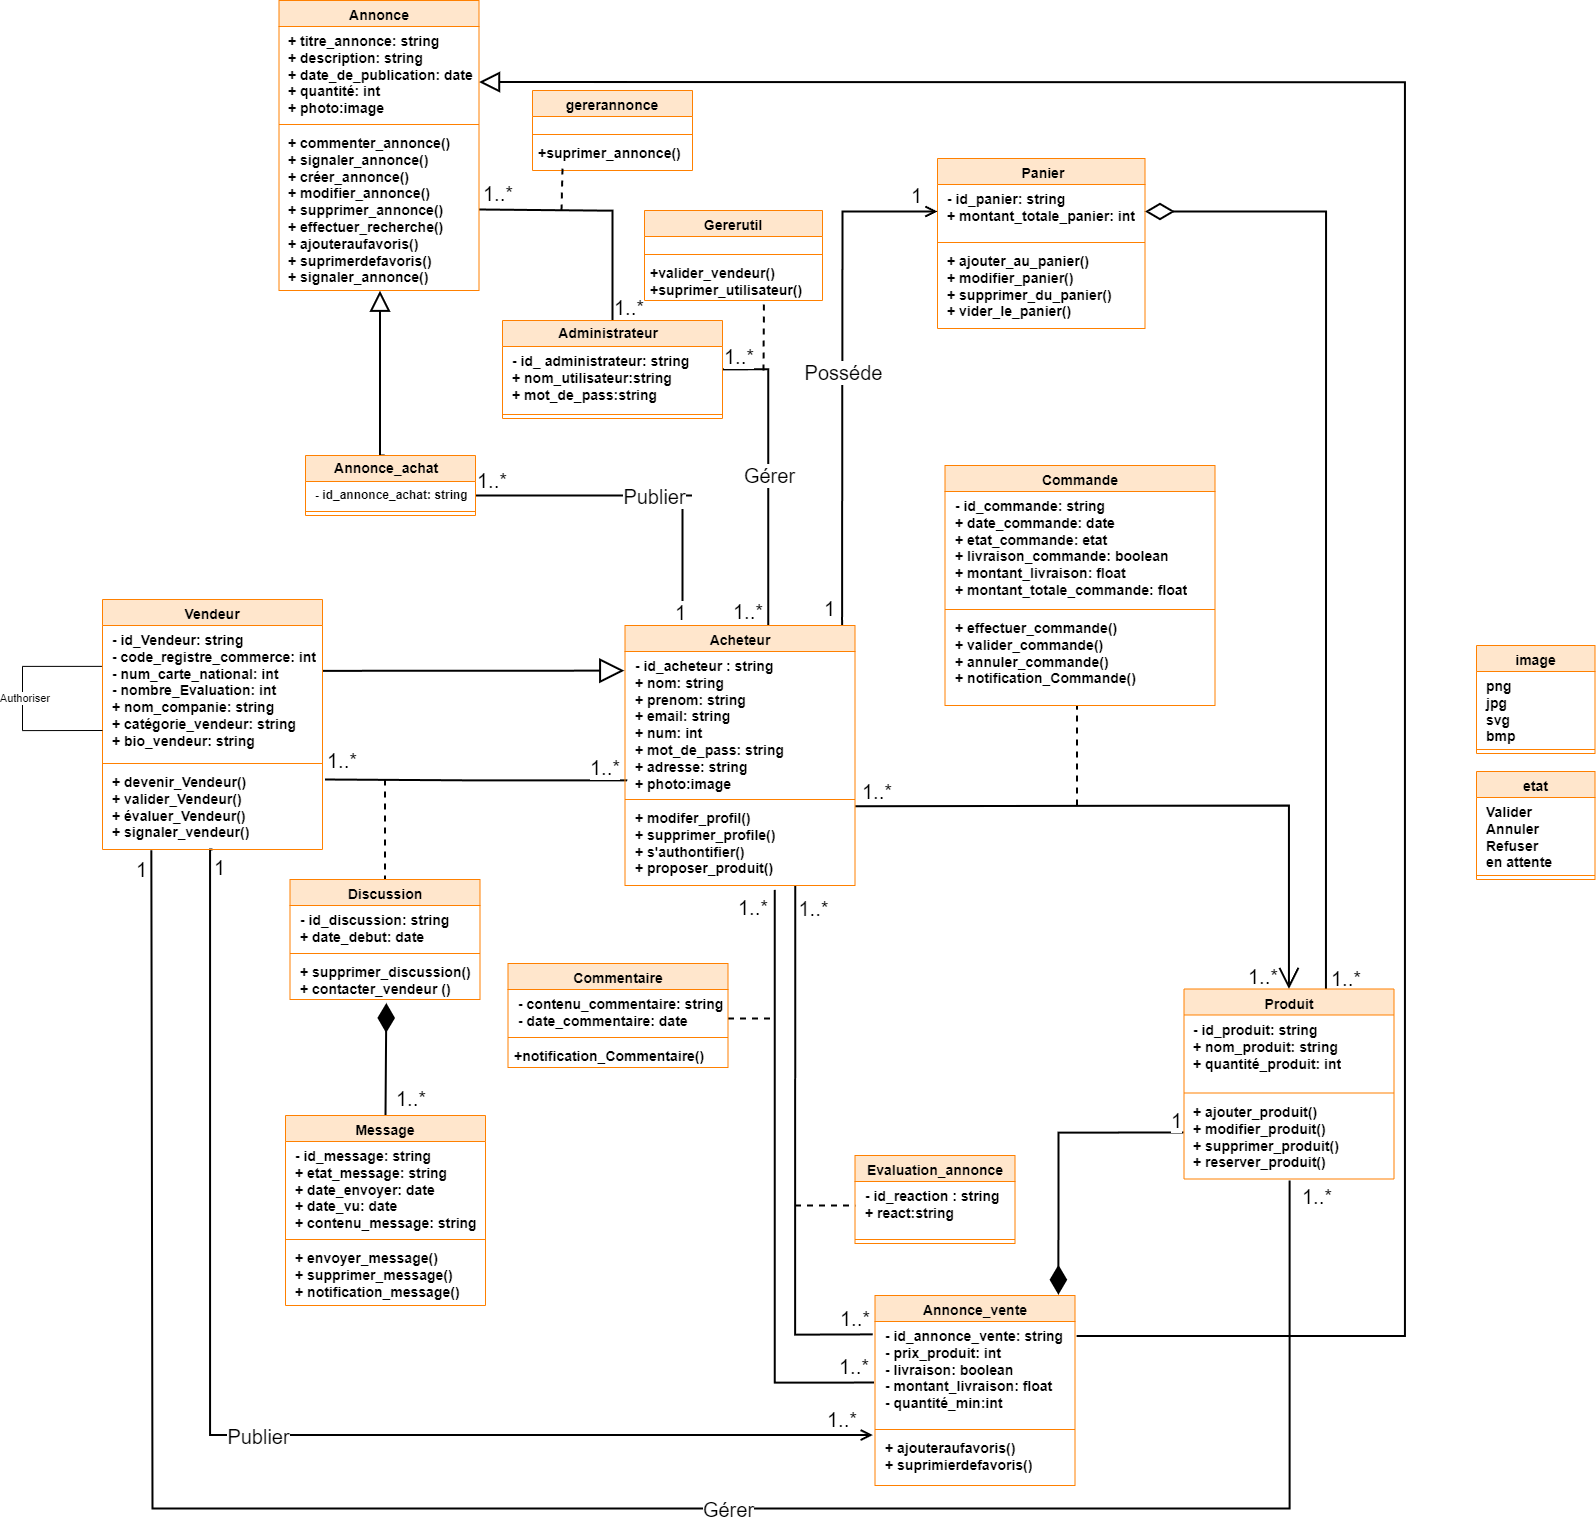
\includegraphics[width=1\textwidth]{images/diagramme de class.png}
\caption{Diagramme de classe}
\end{figure}
\subsection{Passage du diagramme de classes au modèle relationnel }
Pour passer de diagramme de classe vers le modèle relationnel, nous appliquons les règles suivantes :
\newline
\textbf{Règle 1:}Chaque classe devient une table, les attributs de la classe deviennent
les attributs et l’identifiant devient clé primaire pour la table.
\newline
\textbf{Règle 2:}Chaque association 1-1 est prise en compte en incluant la clé primaire
d’une des relations comme clé étrangère dans l’autre relation.
\newline
\textbf{Règle 3:}Chaque association 1-N est prise en compte en incluant la clé comme
clé étrangère dans la relation dont la multiplicité maximale est * la clé primaire
de l’autre relation.
\newline
\textbf{Règle 4:}Chaque association M-N est prise en compte en créant une nouvelle
relation dont la clé primaire est la concaténation des clés primaires de relations
participantes. Les attributs de la classe d’association sont insérés dans cette nouvelle relation si nécessaire.
\newline \phantom{hassane} \newline
En appliquant les règles sur de passage mentionnée dans la partie précédente sur le diagramme de classe suivant (figure: \ref{fig:diag_class}), on obtient le modèle relationnel qui contient les tables suivantes :
\begin{itemize}
    \item administrateur(\underline{id\_administrateur},nom\_utilisateur,mot\_de\_pass)
    \item vendeur(\underline{id\_vendeur},\#id\_panier,code\_registre\_commerce,num\_carte\_national,\newline nombre\_evaluation,nom\_companie,catégorie\_vendeur,bio\_vendeur, nom, prenom, email, num,mot\_de\_pass, adresse, photo)
    \item Acheteur(\underline{id\_acheteur},\#id\_panier, nom, prenom, email, num, mot\_de\_pass, adresse, photo)
    \item gererutil(\#id\_administrateur,\#id\_acheteur,\#id\_vendeur)
    \item gererannonce(\#id\_administrateur,\#id\_annonce\_vente,\#id\_annonce\_achat)
    \item Produit(\underline{id\_produit}, \#id\_vendeur, nom\_produit, quantité\_produit)
    \item Annonce\_vente(\underline{id\_annonce\_vente}, \#id\_produit,\#id\_vendeur, prix\_produit, livraison, montant\_livraison, quantité\_min, titre\_annonce, description, date\_de\_publication, quantité, photo)
    \item annonce\_achat(\underline{id\_annonce\_achat}, \#id\_acheteur, titre\_annonce, description,\newline date\_de\_publication, quantité, Photo)
    \item commentaire(contenu\_commentaire,\#id\_acheteur,\#id\_annonce\_vente, date\_commentaire)
    \item discussion(\underline{id\_discussion}, \#id\_vendeur,\#id\_acheteur, date\_debut)
    \item message(\underline{id\_message},\#id\_discussion,etat\_message,date\_envoyer,date\_vu,contenu\_message)
    \item panier(\underline{id\_panier},montant\_totale panier)
    \item Commande(\underline{id\_commande}, \#id\_acheteur,\#id\_produit, date\_commande, etat\_commande, livraison\_commande, montant\_livraison, montant\_totale\_commande)
    \item evaluation\_annonce(\underline{id\_reaction},react,\#id\_acheteur,\#id\_annonce\_vente)
\end{itemize}
\section{Conclusion}
La phase de conception a concrétisé les besoins identifiés et analysés en une architecture cohérente et structurée. Le diagramme de classe a défini les composants du système et leurs relations, fournissant une base technique robuste pour le développement. Cette étape critique a assuré que le design du système soit en alignement avec les objectifs fonctionnels et non fonctionnels définis précédemment.
%================================
\part{Logiciel de gestion du stock}

\chapter{Expresion des besoins}
\section{Introduction}
Ce Chapitre est dédié à l'identification et à la documentation des besoins spécifiques pour le logiciel de gestion du stock. Cette phase initiale est essentielle pour comprendre les attentes des utilisateurs et les fonctionnalités nécessaires pour répondre aux défis de la gestion des stocks. Nous utilisons des outils comme les diagrammes de cas d'utilisation et de séquence pour visualiser les interactions entre les utilisateurs et le système, garantissant ainsi une compréhension claire et partagée des exigences.
\section{Spécification des besoins}
Cette étape porte sur la compréhension du contexte du système dans lequel nous déterminerons les besoins de notre logiciel de gestion du stock.

Nous avons deux types de besoins : des besoins fonctionnels et des besoins non fonctionnels

\subsection{Les besoins fonctionnels }
Notre logiciel de gestion du stock "EASYCOM" offre un ensemble de fonctionnalités :
\begin{itemize}
    \item \textbf{Gestion des produits:}lPermet la gestion complète des produits, incluant l'ajout, la modification, la suppression et la catégorisation.
    \item \textbf{Suivi des stocks:}Permet la visualisation en temps réel des niveaux de stock, la gestion des seuils de réapprovisionnement et le suivi de l'historique des mouvements.
    \item \textbf{Gestion des commandes:}Permet la gestion complète des commandes fournisseurs et clients, y compris les retours et les échanges
    \item \textbf{Gestion des factures:}Permet la création, le suivi et l'archivage des factures clients et fournisseurs.
    \item \textbf{Rapports et analyses:}Permet de générer des rapports détaillés sur les niveaux de stock, les mouvements et les ventes, et d'analyser les données pour identifier les tendances.
\end{itemize}
\subsection{Les besoins non fonctionnels}
Les besoins non fonctionnels décrivent toutes les contraintes qui doivent être prises en compte afin de mettre en place une meilleure solution pour assurer le bon fonctionnement et la réalisation du système.

Notre application doit nécessairement assure ces besoins
\begin{itemize}
    \item \textbf{L’ergonomie:}l’application doit offrir une interface conviviale et facile pour l’utilisateur.
    \item \textbf{Maintenabilité:}le code doit être lisible pour assurer son état évolutif et faciliter les futures modifications.
    \item \textbf{Rapidité:}le temps de réponse de l’application doit être court.
    \item \textbf{Efficacité:}l’application doit être fonctionnelle indépendamment de toute circonstance pouvant survenir.
    \item \textbf{La sécurité:}tous les accès des utilisateurs doivent être protégés par un login et un mot de passe.
    \item \textbf{L’interface:}Avoir une application qui respecte le principe de \newline l'interface homme/machine tel que l'ergonomie et la fiabilité.
\end{itemize}
\section{ Diagramme de cas d'utilisation }
\subsection{Identification des acteurs et les cas d'utilisations}
\begin{table}[h!]
    \centering
    \begin{tabular}{|c|l|}
    \hline
        L’acteur                  &  Les cas d’utilisations\\ \hline
                                  & Consulter l'historique des achats\\
        Responsable des achats    & Gestion des achats\\
                                  & Gestion des fournisseurs\\ 
                                  & Gestion des annonces  des achat\\\hline
                                  & Consulter l'historique de vente\\
                                  & Gestion des clients\\
                                  & Gestion des commandes clients\\
        Responsable des ventes    & Gestion des paiement\\
                                  & Gestion des factures de vente\\
                                  & Gestion des annonces des vente\\ \hline
                                  & Gestion des depots\\ 
         Gestionnaire de stock    & Gestion des produits\\
                                  & Gestion des familles des produits\\\hline
                                  & Gestion des rôles\\
                                  & Gestion des comptes \\ 
        Superviseur               & Consulter les bénéfices et les chiffres d'affaires\\
                                  & Consulter le mouvement des ventes des produits\\
                                  & connecte au site web  \\\hline
    \end{tabular}
    \caption{Identification des cas d’utilisations}
    \label{tab:Identification des cas d’utilisations}
\end{table}
Nous allons maintenant présenter les diagrammes de cas d'utilisation du logiciel, à la fois général et détaillés.
\newpage
\subsubsection{Diagramme de cas d'utilisation général}
\begin{figure}[h!]\label{fig:Diagramme de cas d'utilisation}
\centering
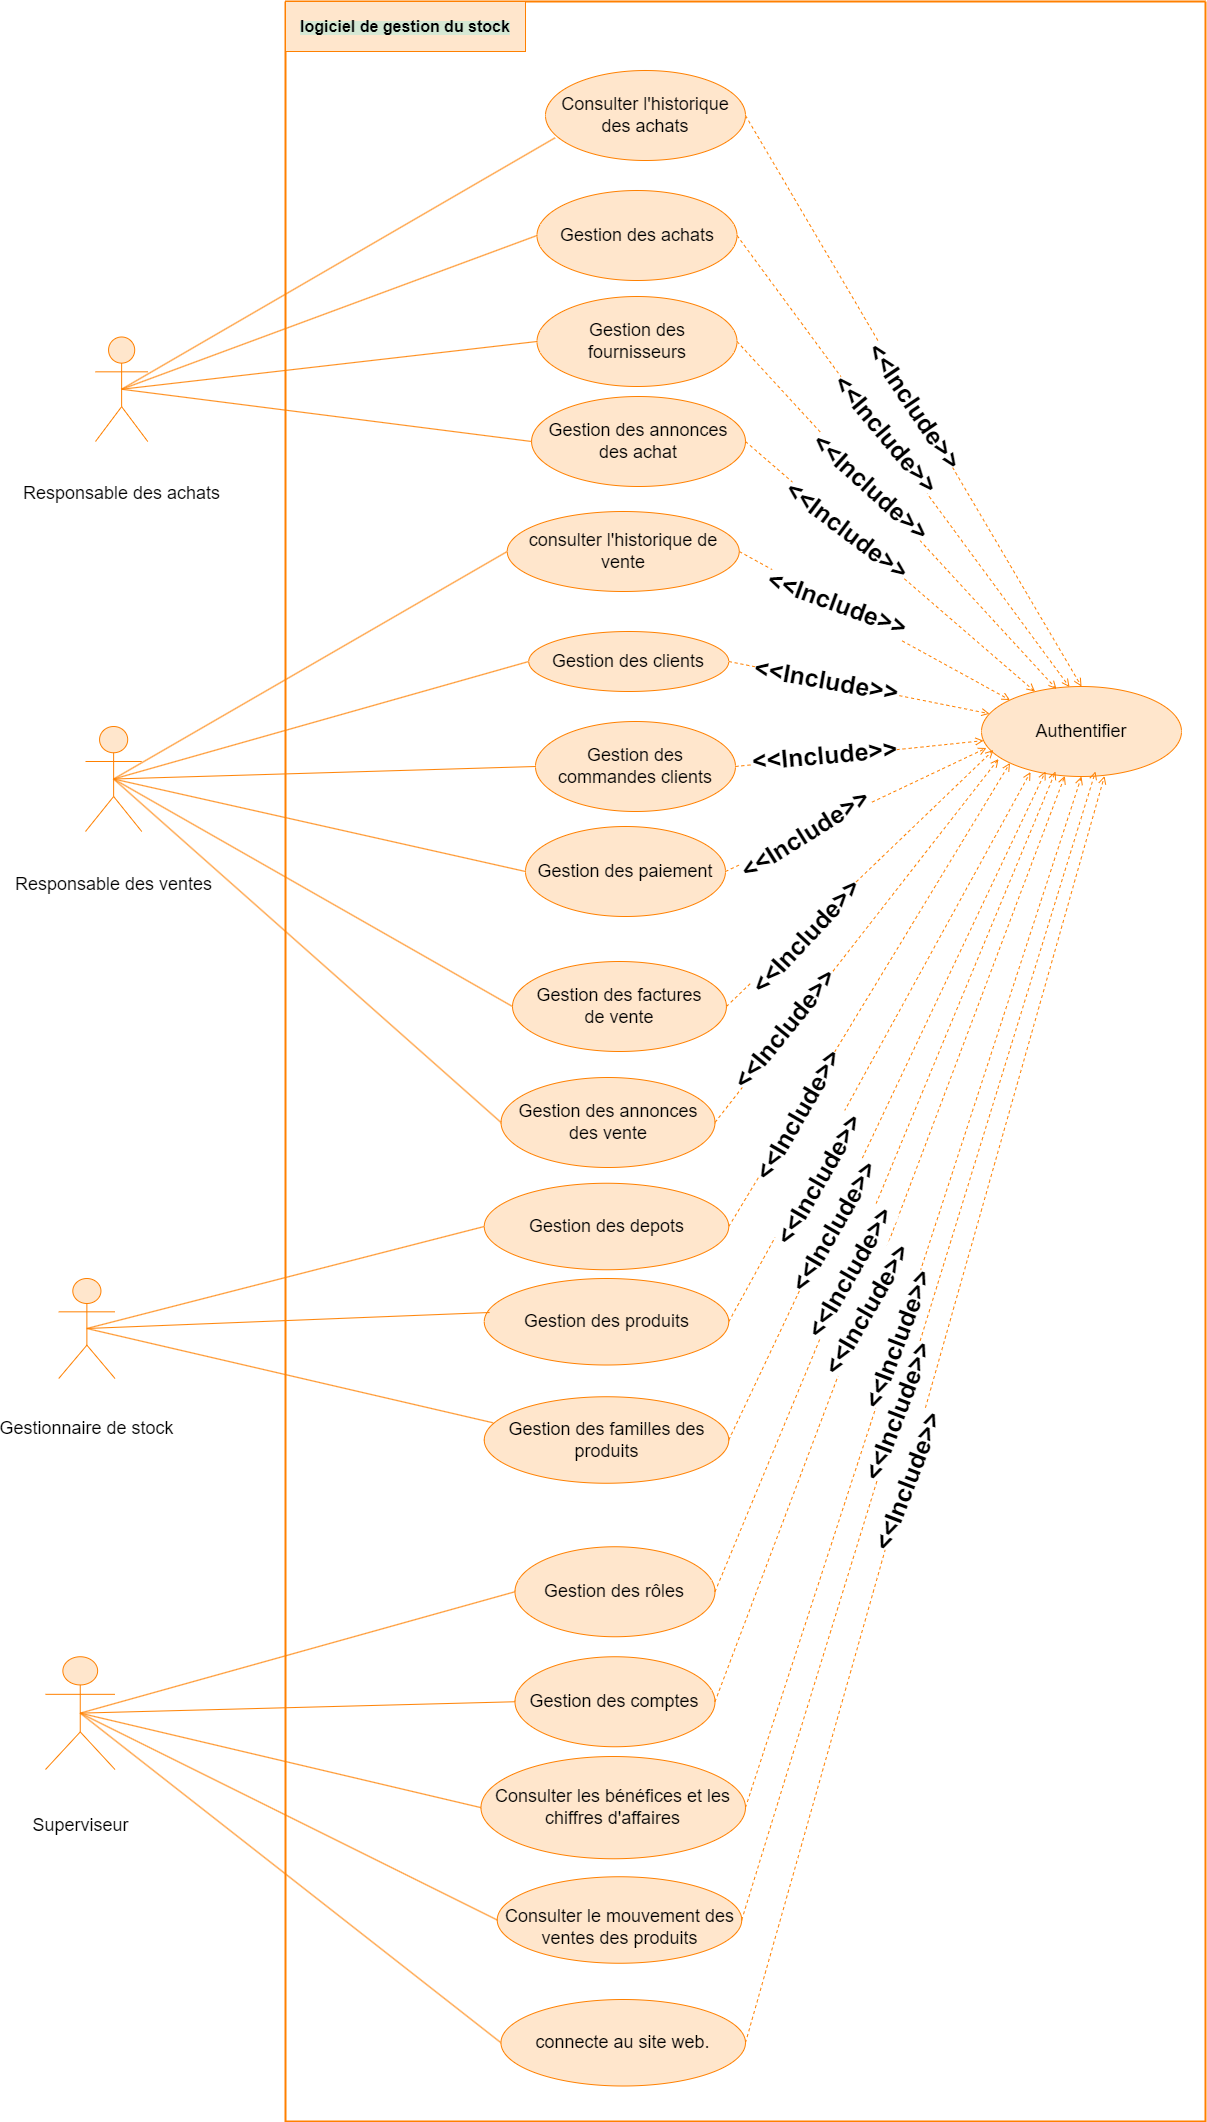
\includegraphics[width=0.7\textwidth]{images/diagramee L G.png}
\caption{Diagramme de cas d'utilisation général}
\end{figure}
\newpage
\subsubsection{Diagramme de cas d'utilisation détailles "superviseur" }
\begin{figure}[h!]\label{fig:diagramme de cas d'utilisation détailles "Superviseur"}
\centering
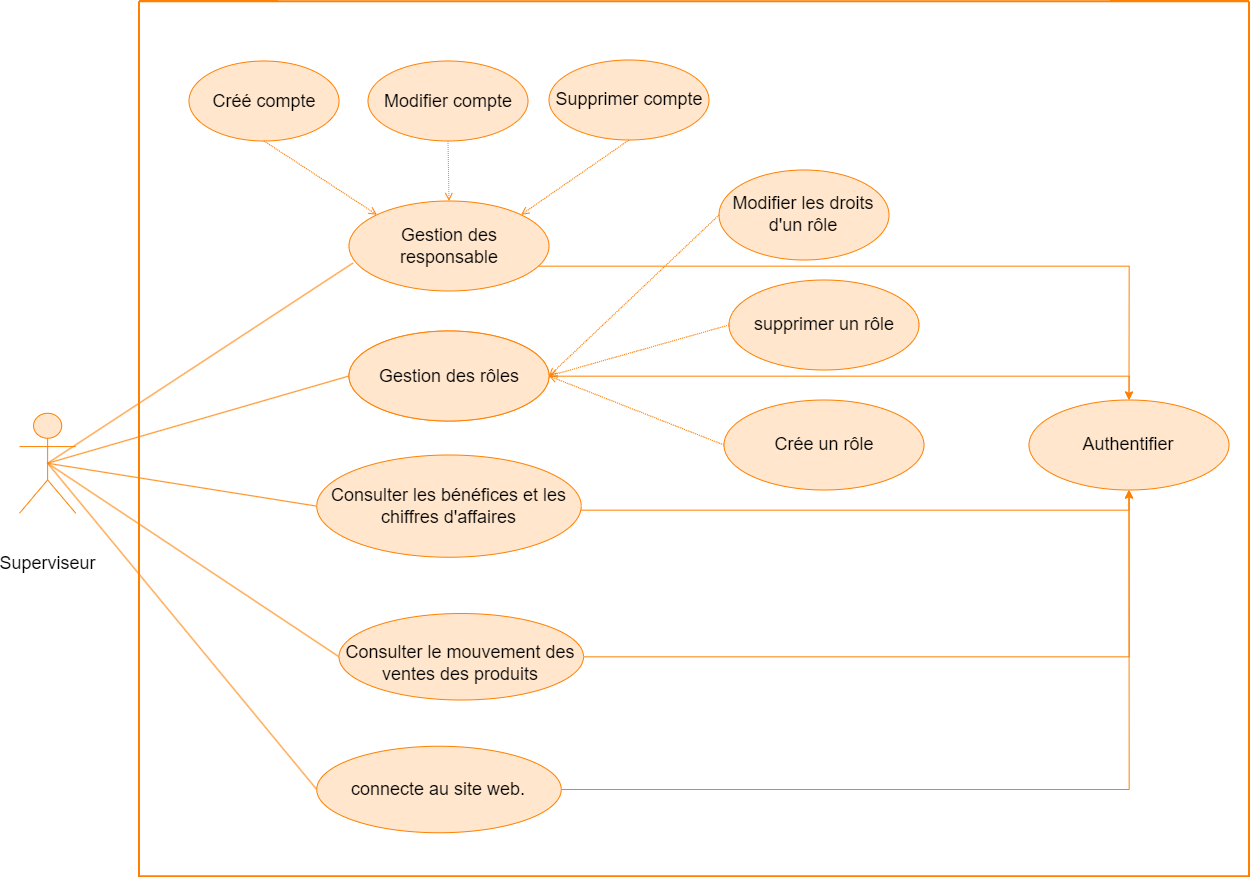
\includegraphics[width=0.7\textwidth]{images/usecase SU.png}
\caption{Diagramme de cas d'utilisation détailles "superviseur"}
\end{figure}
\subsubsection{Diagramme de cas d'utilisation détailles "responsable des achats" }
\begin{figure}[h!]\label{fig:diagramme de cas d'utilisation détailles "responsable des achats"}
\centering
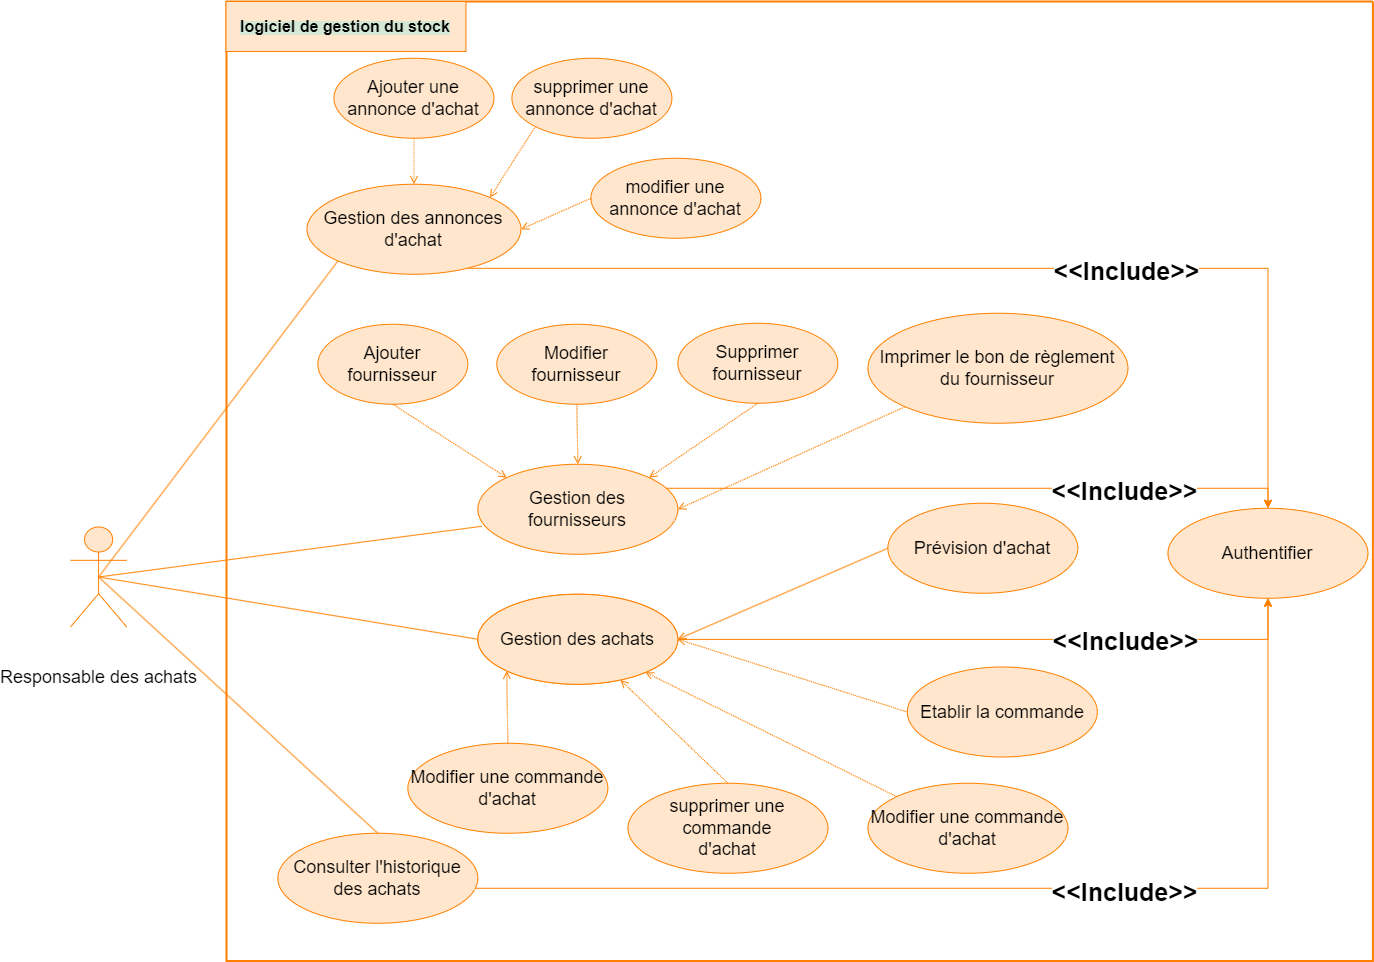
\includegraphics[width=0.7\textwidth]{images/usecas RA.png}
\caption{Diagramme de cas d'utilisation détailles "responsable des achats"}
\end{figure}
\newpage
\subsubsection{Diagramme de cas d'utilisation détailles "responsable des ventes" }
\begin{figure}[h!]\label{fig:diagramme de cas d'utilisation détailles "responsable des ventes"}
\centering
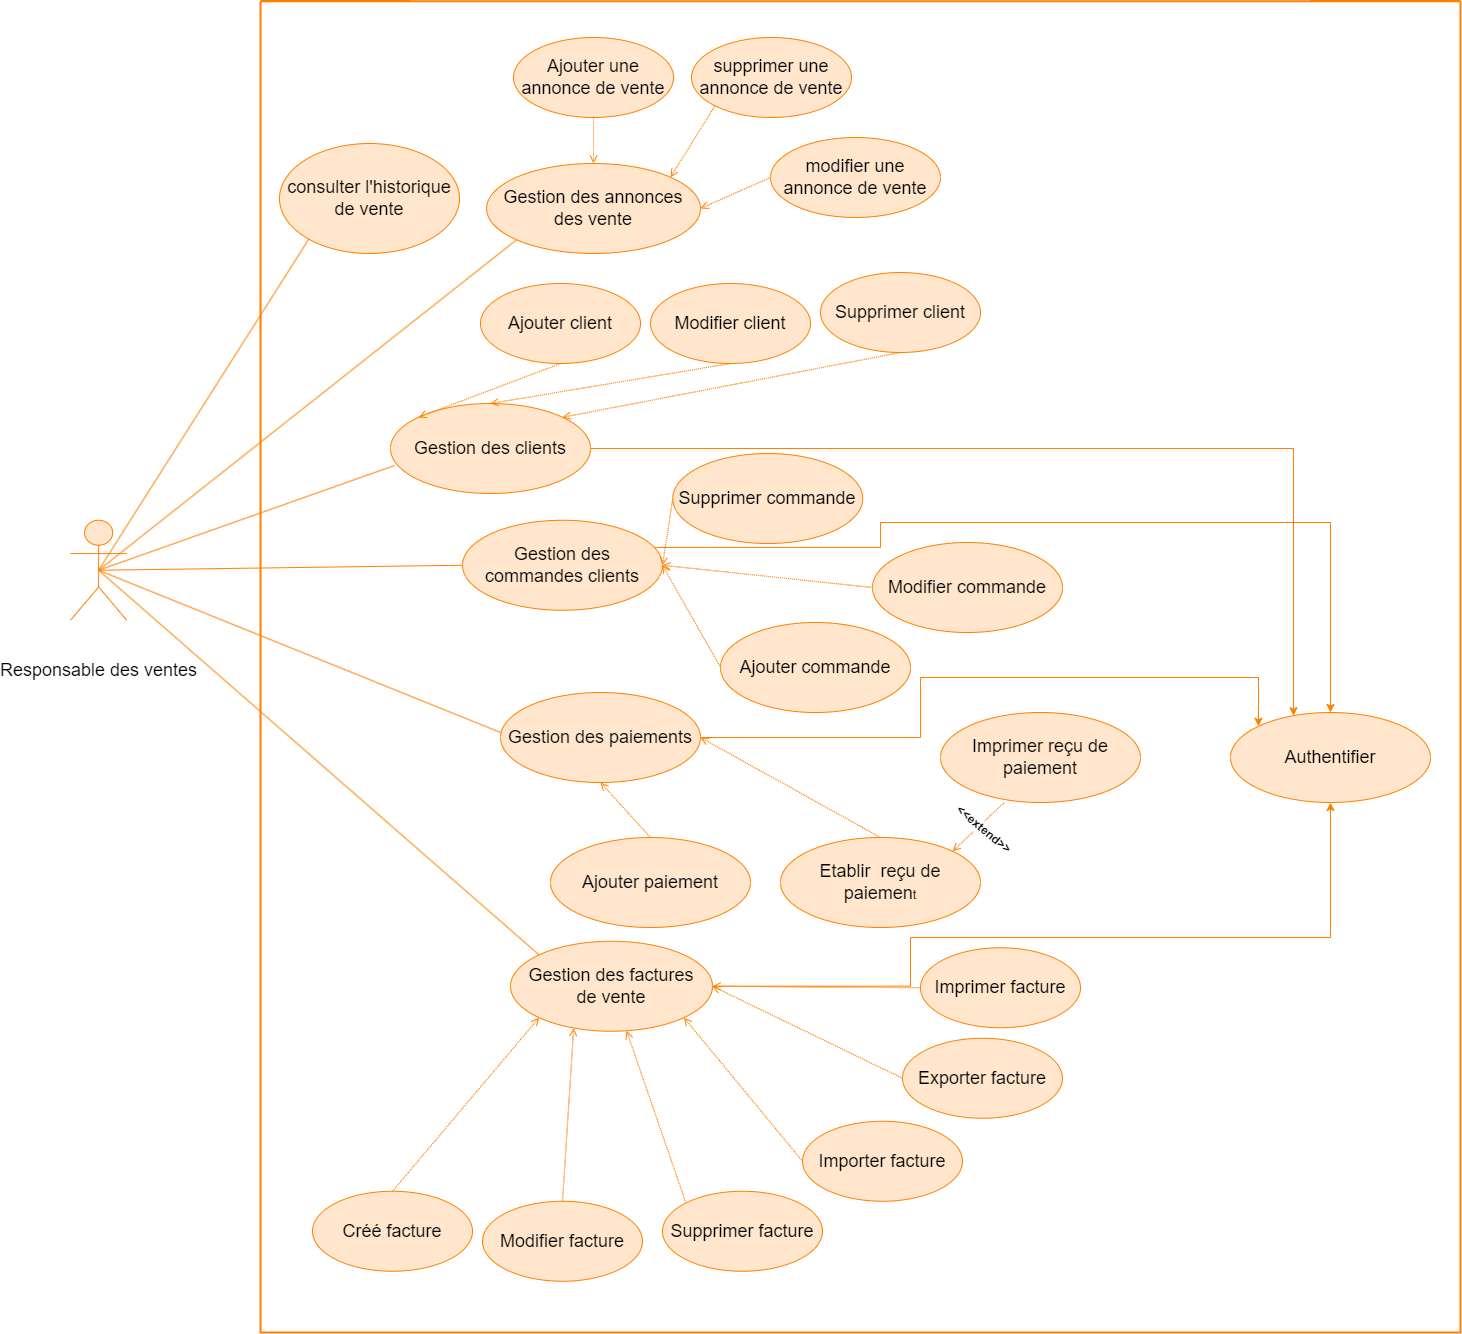
\includegraphics[width=1\textwidth]{images/usecas RV.png}
\caption{Diagramme de cas d'utilisation détailles "responsable des ventes"}
\end{figure}
\newpage
\subsubsection{Diagramme de cas d'utilisation détailles "gestionnaire de stock" }
\begin{figure}[h!]\label{fig:diagramme de cas d'utilisation détailles "Gestionnaire de stock"}
\centering
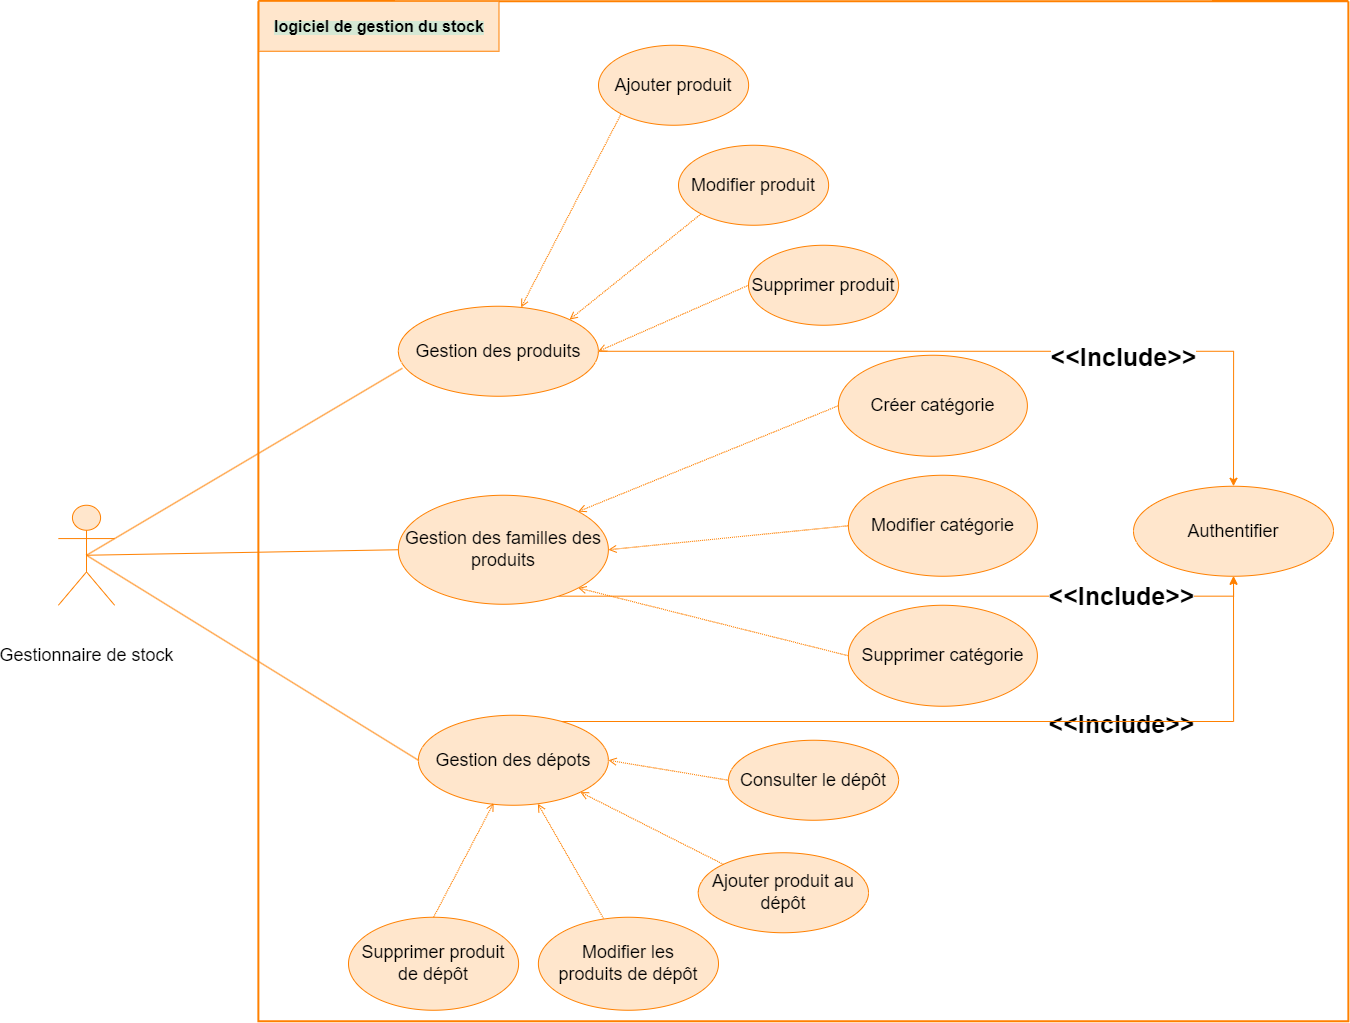
\includegraphics[width=1\textwidth]{images/usecas GS.png}
\caption{Diagramme de cas d'utilisation détailles "gestionnaire de stock"}
\end{figure}\clearpage


\section{Diagrammes de séquences}
Voici quelques exemples de diagrammes de séquence pour des cas d'utilisation importants que nous allons présenter ci-dessous.
\subsubsection{Cas d'utilisation "ajouter client"}
\begin{table}[h!]
    \centering
\begin{tabular}{|c|m{10cm}|}
    \hline
         \multicolumn{2}{|c|}{Identification du cas d'utilisation "ajouter client" }\\
         \hline
         Acteur & Responsable des ventes\\
         \hline
         Pré-condition & L'utilisateur doit être authentifié en tant que Responsable des ventes. \\
         \hline
          & 1- l'utilisateur demande le menu.\\
          & 2- le système affiche le menu. \\
          & 3- l'utilisateur demande la liste des clients.\\
          Scénario & 4- le système affiche la liste des clients. \\          
          nominal& 5- l'utilisateur demande l’ajout d’un nouveaux client.\\
          & 6- le système affiche le formulaire pour ajouter un client \\
          & 7- l'utilisateur remplit le formulaire et valide les informations du client \\
          & 8- le système vérifie la validité des informations saisies\\
          & 9- Le système affiche un message de succès, ainsi il ajoute un nouveau client.\\
         \hline
         Alternative  & A l’étape 8 si un champ d’information n’est pas valide,  \\
         & le système affiche un message d’erreur.\\
         \hline
         Post condition& L’ajout de client avec succès \\
         \hline
    \end{tabular}
\caption{Description textuelle du cas d'utilisation "ajouter client"}
\label{tab:aj}
\end{table}
\begin{figure}[h!]\label{fig:ajouter}
\centering
\includegraphics[width=0.8\textwidth]{images/seq ajouter client.png}
\caption{Diagramme de séquence du cas d'utilisation "ajouter client"}
\end{figure}

\clearpage
\subsubsection{Cas d'utilisation "ajouter commande"}
\begin{table}[h!]
    \centering
    \begin{tabular}{|c|m{10cm}|}
        \hline
             \multicolumn{2}{|c|}{Identification du cas d'utilisation "ajouter commande" }\\
             \hline
             Acteur & Responsable des ventes\\
             \hline
             Pré-condition & L'utilisateur doit être authentifié en tant que Responsable des ventes. \\
             \hline
              & 1- l'utilisateur demande le menu.\\
              & 2- le système affiche le menu. \\
              & 3- l'utilisateur demande la liste des commandes.\\
              Scénario& 4- le système affiche la liste des commandes. \\ 
              nominal& 5- l'utilisateur demande d'établir une commande.\\
              & 6- le système affiche le formulaire pour établir une commande. \\
              & 7- l'utilisateur remplit le formulaire et valide les informations du la commande. \\
              & 8- le système vérifie la validité des informations saisies\\
              & 9- Le système affiche un message de succès, ainsi il ajoute une nouvelle commande.\\
              
             \hline
             Alternative  & A l’étape 8 si un champ d’information n’est pas valide,  \\
             & le système affiche un message d’erreur.\\
             \hline
             Post condition& L’ajout de la commande avec succès \\
             \hline
        \end{tabular}
    \caption{Description textuelle du cas d'utilisation "ajouter commande"}
    \label{tab:cas1}
\end{table}
\begin{figure}[h!]\label{fig:Diagramme cas1}
\centering
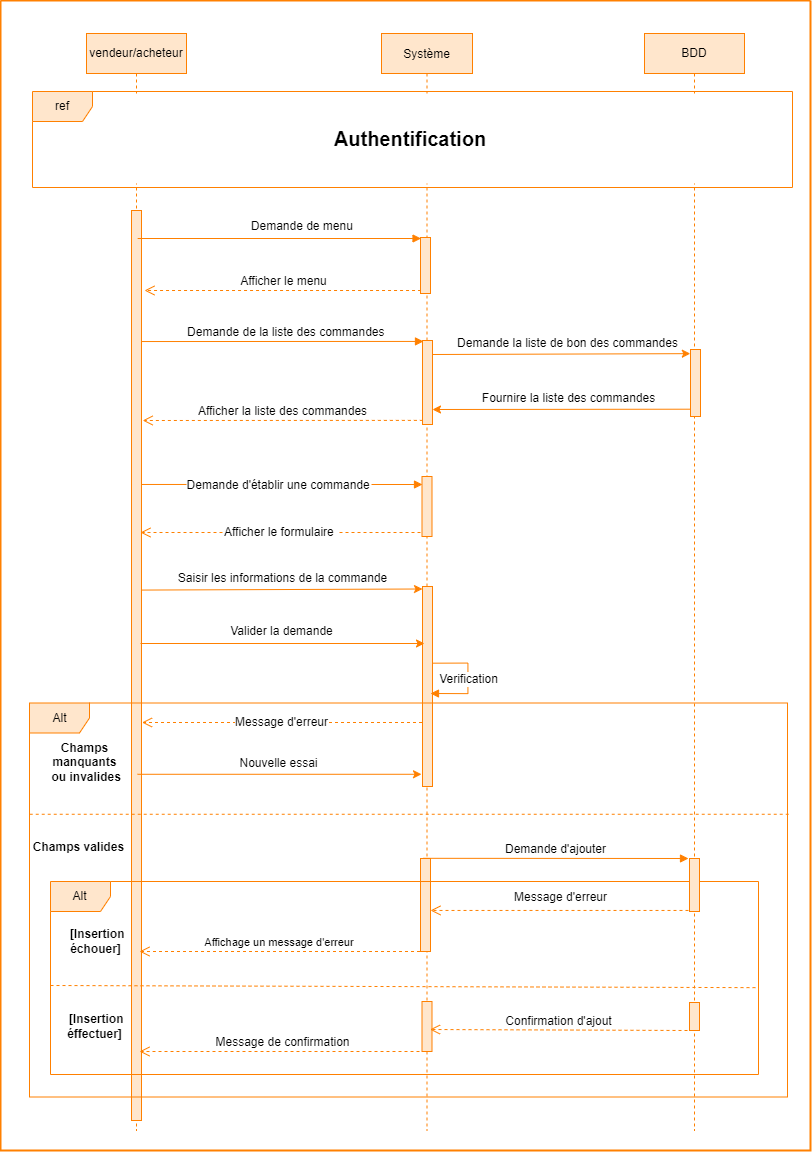
\includegraphics[width=1\textwidth]{images/seq etablier commande.png}
\caption{Diagramme de séquence du cas d'utilisation "ajouter commande"}
\end{figure}

\clearpage
\subsubsection{Cas d'utilisation "imprimer bon de commande"}
\begin{table}[h!]
    \centering
    \begin{tabular}{|c|m{10cm}|}
        \hline
             \multicolumn{2}{|c|}{Identification du cas d'utilisation "imprimer bon de commande" }\\
             \hline
             Acteur & Responsable des ventes\\
             \hline
             Pré-condition & L'utilisateur doit être authentifié en tant que responsable des ventes. \\
             \hline
              & 1- l'utilisateur demande le menu.\\
              & 2- le système affiche le menu. \\
              & 3- l'utilisateur demande la liste des commandes.\\
              & 4- le système affiche la liste des commandes. \\          
              Scénario&  5- l'utilisateur demande les details d'une commande.\\
              nominal & 6- le système affiche les details de la commande. \\
              & 7- l'utilisateur demande d'imprimer de bon de commande. \\
              & 8- le système affiche le bon avec une confirmation d'impression. \\
              & 9- L'utilisateur valide avec oui.\\
              & 10- Le système imprime le bon et affiche un message de succès.\\
             \hline
             Alternative  & A l’étape 9 si l'utilisateur valide avec non, \\
             & le système va annuler l'impression.\\
             \hline
             Post condition& L’impression de bon de commande avec succès \\
             \hline
        \end{tabular}
    \caption{Description textuelle du cas d'utilisation "impression d'un bon de commande"}
    \label{tab:cas1}
\end{table}
\begin{figure}[h!]\label{fig:Diagramme cas1}
\centering
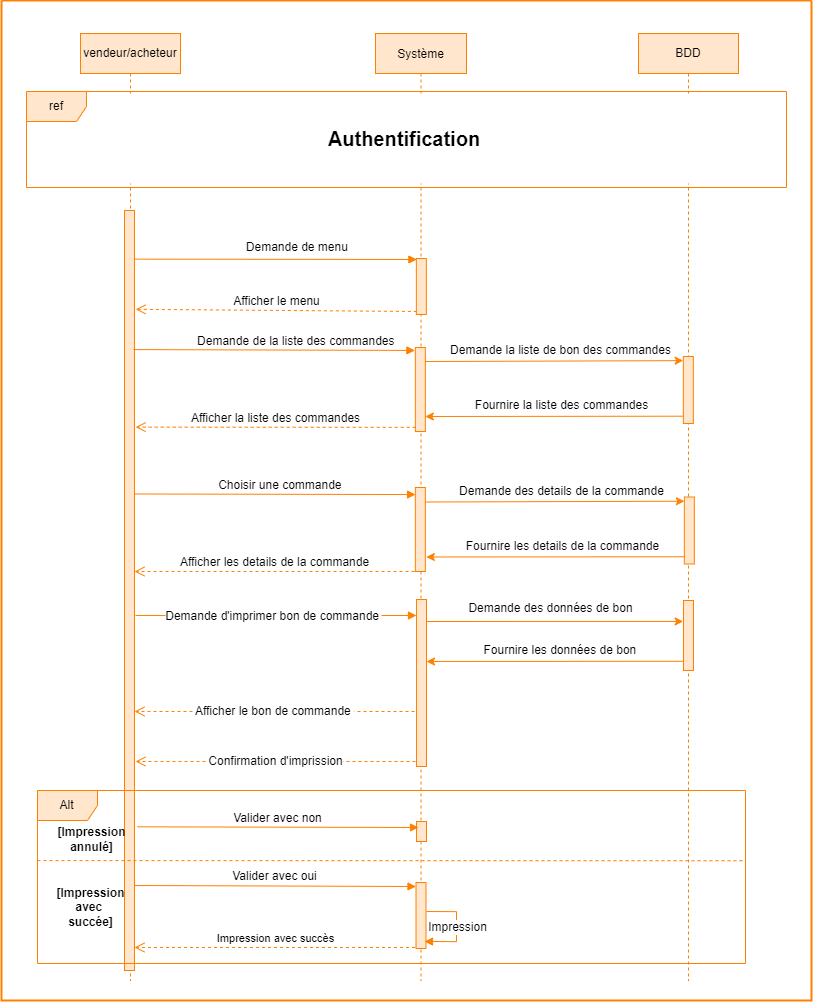
\includegraphics[width=1\textwidth]{images/seq imprimer bon de commande.png}
\caption{Diagramme de séquence du cas d'utilisation "imprimer bon de commande"}
\end{figure}

\clearpage
\subsubsection{Cas d'utilisation "ajouter un produit au stock"}
\begin{table}[h!]
    \centering
    \begin{tabular}{|c|m{10cm}|}
        \hline
             \multicolumn{2}{|c|}{Identification du cas d'utilisation "ajouter un produit au stock"}\\
             \hline
             Acteur & Gestionnaire de stock\\
             \hline
             Pré-condition & L'utilisateur doit être authentifié en tant que gestionnaire de stock, est superviseur doit être authentifié au site-web. \\
             \hline
              & 1- l'utilisateur demande le menu.\\
              & 2- le système affiche le menu. \\
              & 3- l'utilisateur demande la liste des produits.\\
              Scénario& 4- le système affiche la liste des produits. \\          
              nominal& 5- l'utilisateur demande l’ajout d’un nouveaux produits au stock.\\
              & 6- le système affiche le formulaire pour ajouter un produit \\
              & 7- l'utilisateur remplit le formulaire et valide les informations du produit \\
              & 8- le système vérifie la validité des informations saisies\\
              & 9- Le système affiche un message de succès, ainsi il ajoute un nouveau produit au stock.\\
             \hline
             Alternative  & A l’étape 8 si un champ d’information n’est pas valide,  \\
             & le système affiche un message d’erreur.\\
             \hline
             Post condition& L’ajout de produit avec succès \\
             \hline
        \end{tabular}
    \caption{Description textuelle du cas d'utilisation "ajouter un produit au stock"}
    \label{tab:cas1}
\end{table}
\begin{figure}[h!]\label{fig:Diagramme cas1}
\centering
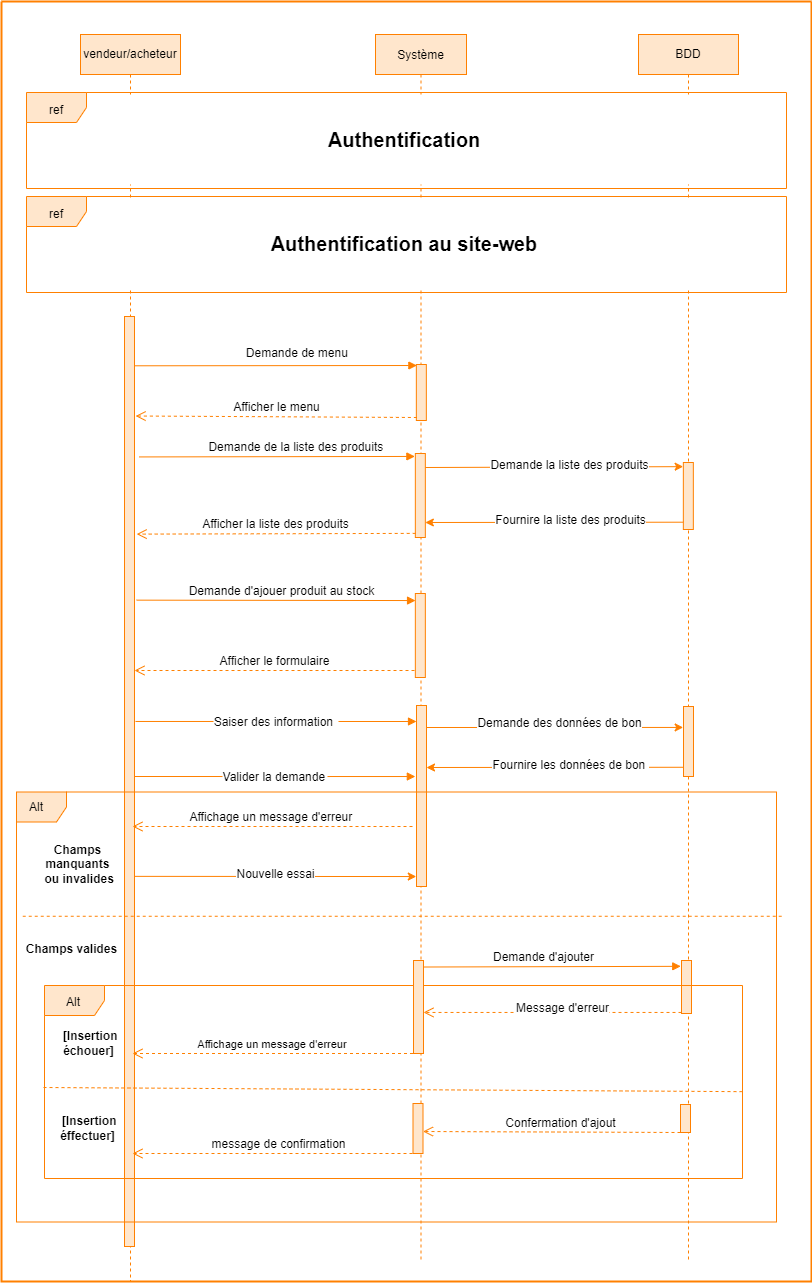
\includegraphics[width=1\textwidth]{images/seq ajouter un produit au stock.png}
\caption{Diagramme de séquence du cas d'utilisation "ajouter un produit au stock"}
\end{figure}
\clearpage
\section{Conclusion}
Pour le logiciel de gestion du stock, ce chapitre a clarifié les besoins spécifiques en termes de gestion des stocks, suivi des inventaires et optimisation des ressources. Les diagrammes de cas d'utilisation et de séquence ont aidé à identifier les principales fonctionnalités et les interactions utilisateurs, assurant que toutes les exigences métiers soient capturées et comprises.


%====================================>
\chapter{Analyse des besoins}
\section{Introduction}
Dans ce chapitre nous approfondissons les besoins identifiés dans le chapitre précédent. L'analyse détaillée permet de décomposer chaque exigence en éléments plus précis et de comprendre les flux de travail associés. Les diagrammes de séquence détaillés et les diagrammes d'activité sont utilisés pour modéliser les processus métiers, identifier les inefficacités et proposer des améliorations. Cette phase critique prépare le terrain pour une conception technique robuste et bien informée.
\section{Diagramme d'activité}
Dans les sections suivantes, nous présenterons divers exemples de diagrammes d'activité pour plusieurs cas d'utilisation.
\subsubsection{Cas d'utilisation "ajouter utilisateur"}
\begin{figure}[h!]\label{fig:activite utilisateur}
    \centering
    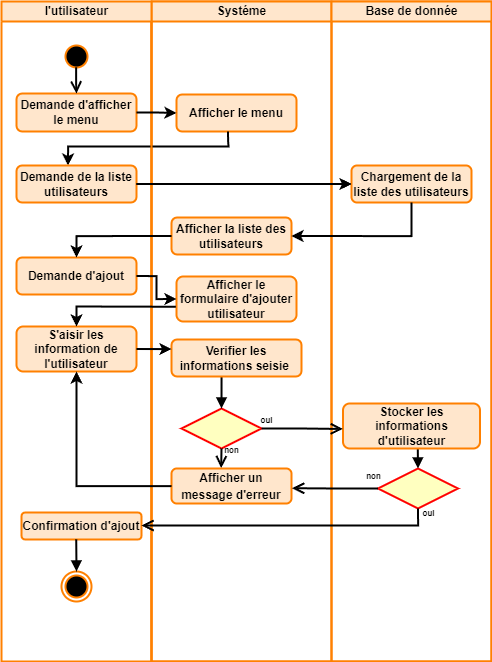
\includegraphics[width=0.9\textwidth]{images/act ajouter utilisateur.png}
    \caption{Diagramme d'activité "ajouter utilisateur"}
\end{figure}

\clearpage
\subsubsection{Cas d'utilisation "modifier client"}
\begin{figure}[h!]\label{fig:activite modiciferc}
    \centering
    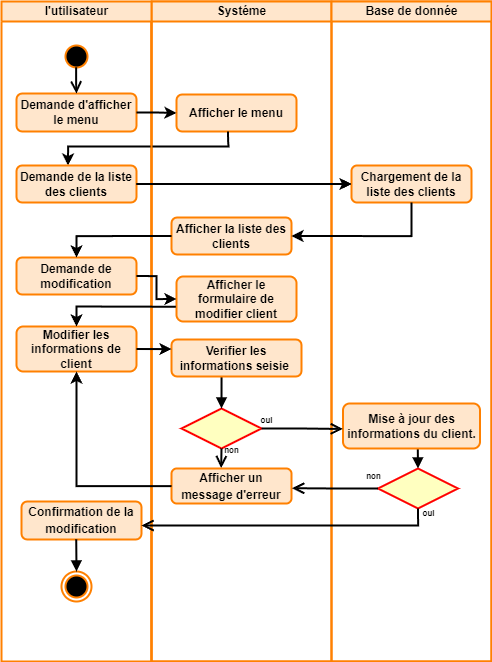
\includegraphics[width=1\textwidth]{images/act modifier client.png}
    \caption{Diagramme d'activité "modifier client"}
\end{figure}

\clearpage
\subsubsection{Cas d'utilisation "ajouter produit au stock de platforme Web"}
\begin{figure}[h!]\label{fig:activite ajouters}
    \centering
    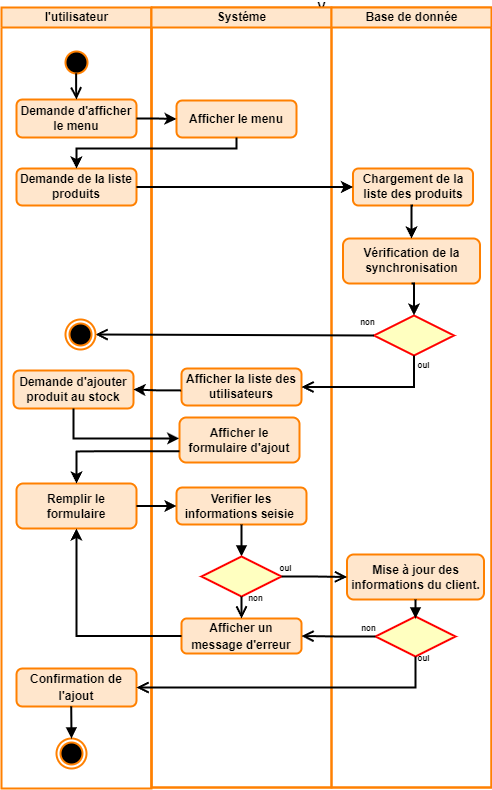
\includegraphics[width=0.8\textwidth]{images/act ajouter produit au stock.png}
    \caption{Ddiagramme d'activité "ajouter produit au stock de platforme Web"}
\end{figure}

\clearpage
\subsubsection{Cas d'utilisation "publier une annonce sur la platforme web"}
\begin{figure}[h!]\label{fig:activite publier}
    \centering
    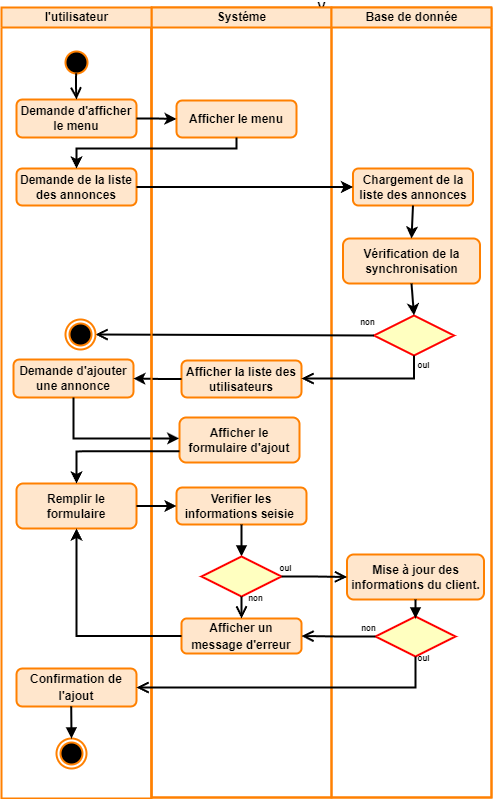
\includegraphics[width=0.8\textwidth]{images/act Publier une annonce sur la platforme web.png}
    \caption{Diagramme d'activité "publier une annonce sur la platforme web"}
\end{figure}
\clearpage



\section{Les diagrammes de séquence détaillé}
Dans ce qui suit, nous allons détailler les diagrammes de séquence pour quelques cas d'utilisation.
\subsubsection{Cas d'utilisation "authentification au site détaillé"}
\begin{figure}[h!]\label{fig:Authentification au site}
\centering
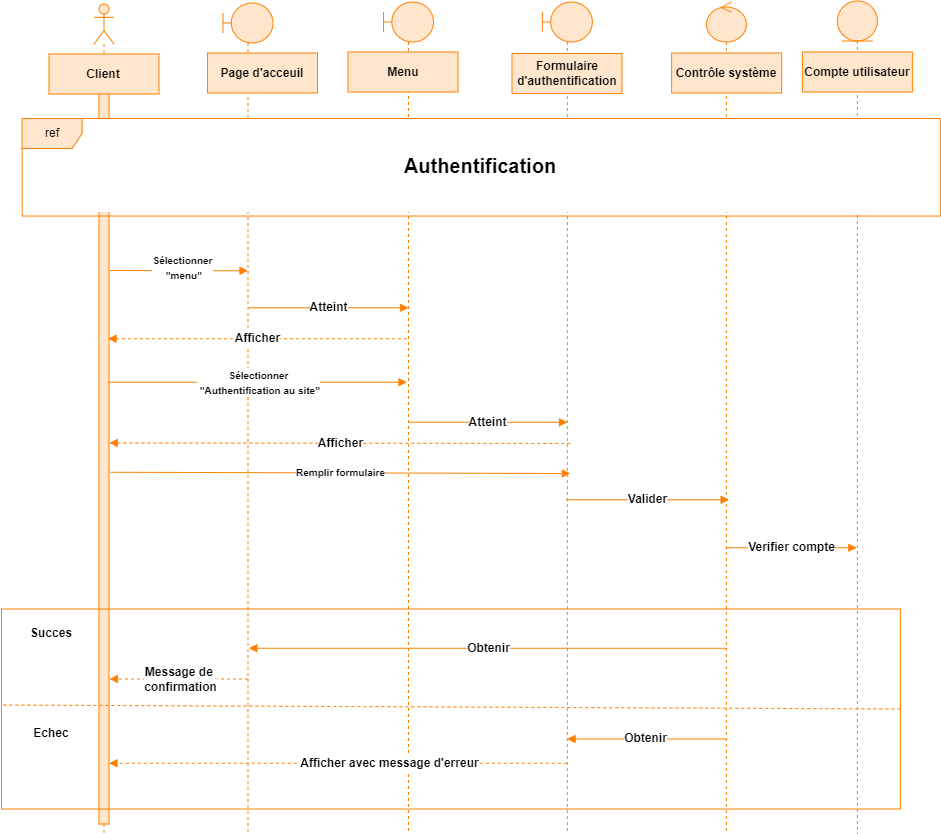
\includegraphics[width=0.8\textwidth]{images/Authentification au site.png}
\caption{Dagramme de séquence du cas d'utilisation "authentification au site détaillé"}
\end{figure}
\clearpage

\subsubsection{Cas d'utilisation "etablir commande détaillé"}
\begin{figure}[h!]\label{fig:etablir commande}
\centering
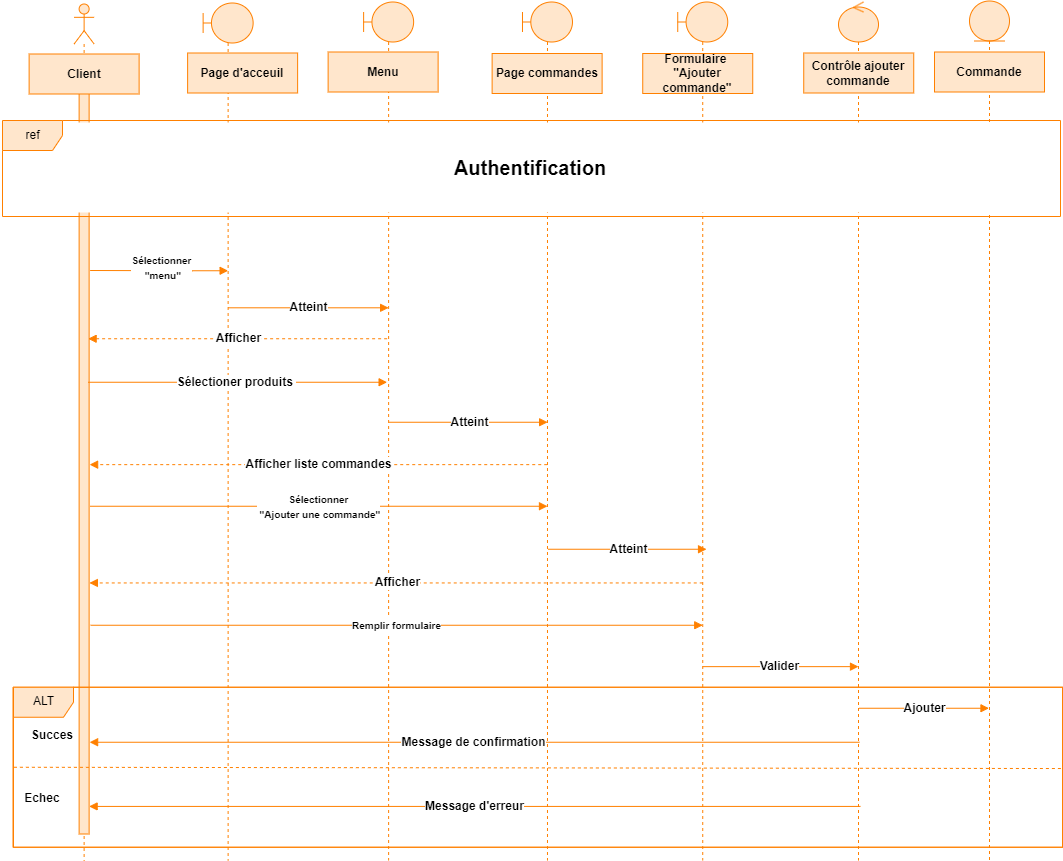
\includegraphics[width=0.8\textwidth]{images/Cas_ etablir commande.png}
\caption{Diagramme de séquence du cas d'utilisation "etablir commande détaillé"}
\end{figure}
\clearpage

\subsubsection{Cas d'utilisation "ajouter un produit au stock de platforme Web détaillé"}
\begin{figure}[h!]\label{fig:Ajouter un produit au stock de site Web}
\centering
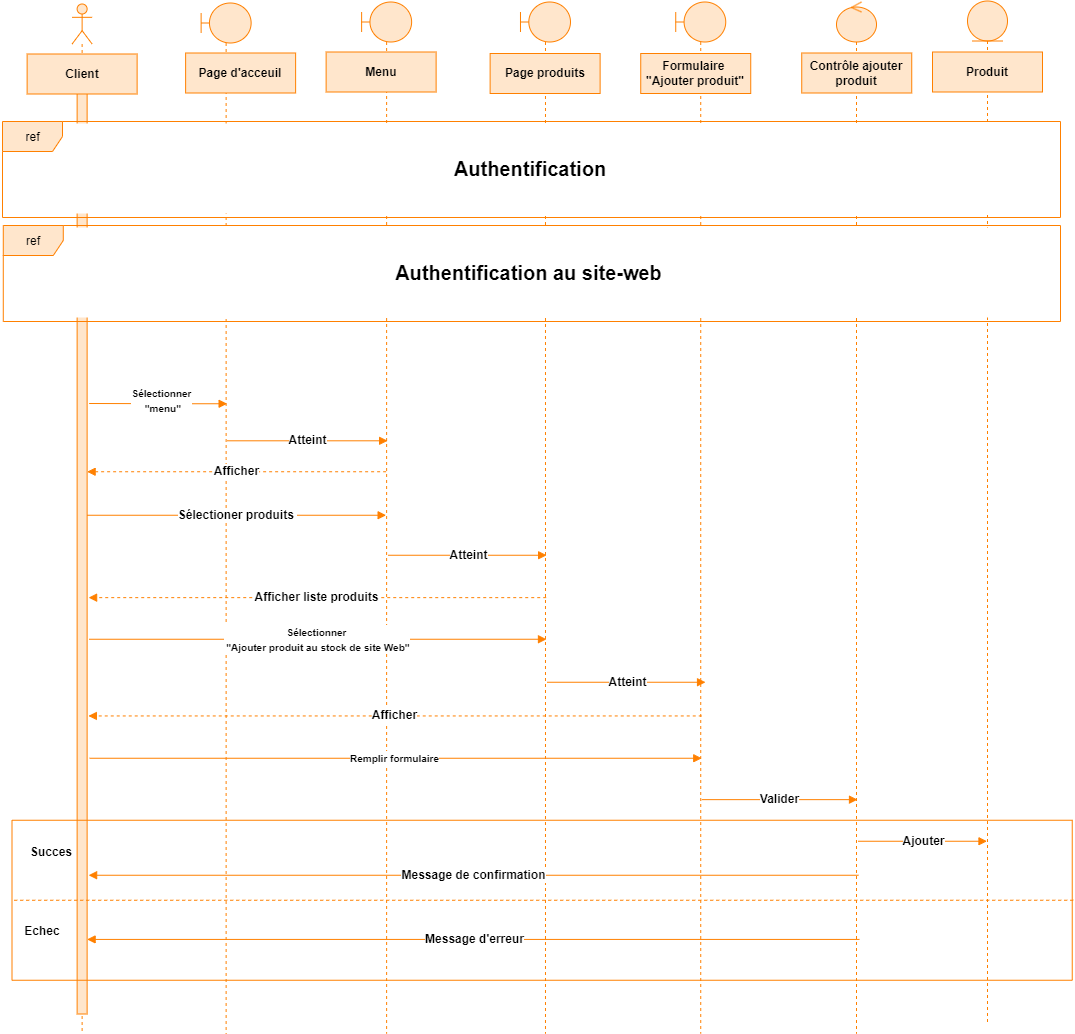
\includegraphics[width=0.8\textwidth]{images/Cas_ Ajouter un produit au stock de site Web.png}
\caption{Diagramme de séquence du cas d'utilisation "ajouter un produit au stock de platforme Web détaillé"}
\end{figure}
\section{Conclusion}
L'analyse détaillée des besoins pour le logiciel de gestion du stock a permis de décomposer et d'examiner les processus en profondeur. Les diagrammes de séquence détaillés et d'activité ont fourni une vue claire des flux de travail, permettant d'identifier les inefficacités et les points d'amélioration. Cela a préparé le terrain pour une conception optimisée et bien informée.
%==========================>
\chapter{Conception}
\section{Introduction}
Ce chapitre concentre sur la transformation des besoins analysés en une architecture logicielle cohérente et structurée. À travers l'utilisation de diagrammes de classe, nous définissons les composants du système, leurs relations et leurs interactions. Cette phase de conception vise à assurer que le logiciel de gestion du stock soit non seulement fonctionnel et efficace, mais aussi extensible et maintenable. La conception bien pensée pose les bases d'un développement réussi et d'une mise en œuvre fluide du logiciel.
\section{diagramme de classe}
\subsection{Dictionnaire de données}
Le dictionnaire des données est un document qui regroupe toutes les données que vous
aurez à conserver dans votre base. Pour chaque donnée, il indique le code mnémonique,la
désignation, le type de donnée
\newline Le tableau suivant représente le dictionnaire de données de notre système 
\begin{table}[h!]
    \centering
    \begin{tabular}{ | m{2,6cm} | m{3,2cm}| m{3cm} |m{0,9cm}|m{0,9cm}|l|}
    \hline
         Classe&\multicolumn{3}{c}{Attributs}&\phantom{h} &Methodes\\
         \hline &Nom&Description&Type&Taille&\\\cline{2-5}
                                        &id\_client    &l'id de client&AN&15& \\\cline{2-6}
                                        &nom\_client   &le nom de client&A&15&Ajouterclient() \\\cline{2-6}
                                        &prénom\_client&le prenom de client&A&15&supprimerclient() \\\cline{2-6}
                            Client      &mail\_client  &l'email de client&AN&30&modifierclient() \\\cline{2-6}
                                        &numclient    &le numéro de client&N&10&\\\cline{2-5}
                                        &addresse\_client&l'Adresse de client&AN&30&\\\hline
                                        

                                        
                            Responsable &nom\_resp &le nom de responsable&AN&15&ajouter\_resp()\\\cline{2-6}
                            &mot\_de\_pass\_res&le mot de pass de responsable&N&20&supprimer\_resp()\\\hline

                

 \end{tabular}
 
\end{table}
\begin{table}[H]
    \centering
    \begin{tabular}{ | m{2,6cm} | m{3,2cm}| m{3cm} |m{0,9cm}|m{0,9cm}|l|}
    \hline
         Classe&\multicolumn{3}{c}{Attributs}&\phantom{h} &Methodes\\
         \hline &Nom&Description&Type&Taille&\\\cline{2-5}
         Respensable des ventes  &id\_resp\_vents&l'id de discussion&AN&15&vendre() \\\hline
        Respensable des achats  &id\_resp\_achat&l'id de discussion&AN&15&acheter() \\\hline
         
        Respensable de stock    &id\_resp\_stk&l'id de discussion&AN&15& \\\hline


                    &id\_fourni    &l'id de fournisseur&AN&15& \\\cline{2-6}
                    &nom\_fourni   &le nom de fournisseur&A&15&ajouterfourni() \\\cline{2-6}
                    &prénom\_fourni&le prenom de fournisseur&A&15&supprimerfourni() \\\cline{2-6}
        Fournisseur &mail\_fourni  &l'email de fournisseur&AN&30&modifierfourni() \\\cline{2-6}
                    &num\_fourni   &le numéro de fournisseur&N&10&\\\cline{2-5}
                    &address\_fourni&l'addresse de fournisseur&AN&30&\\\hline

                    &id\_prod    &l'id de produit&AN&15& \\\cline{2-6}
                    &lot\_prod   &le lot de produit&An&15&ajouterprod() \\\cline{2-6}
                    &date\_ex\_p &la date d'expiration de produit&date&8&supprimerprod() \\\cline{2-6}
        Produit     &prix\_achat &prix d'achat de produit&N&30&modifierprod() \\\cline{2-6}
                    &prix\_vent  &prix de vent de produit&N&30&\\\cline{2-5}
                    &qte\_prod   &la quantité de produit&N&30&\\\hline

                    
                    &id\_bl &l'id de bon de livraison&AN&15& Créerbl()\\\cline{2-6}
    Bon de livraison&date\_liv &la date de livraison&date&8&Imprimerbl()\\\cline{2-6}
                    &qte\_prod\_liv&la quantité de produit Livrer&N&20&\\\hline
                    

                    &id\_achat  &l'id d'achat&AN&15&ajouterachat()\\\cline{2-6}
    Achat           &date\_achat&la date d'achat&date&8&modifierachat()\\\cline{2-6}
                    &qte\_prod  &la quantité de produit achate&N&20&supprimerachat()\\\cline{2-6}
                    &num\_achat &le numéro d'achat            &N&10&Imprimerfactureachat()\\\hline

                    &id\_vent  &l'id de vente&AN&15&ajoutervent()\\\cline{2-6}
    Vente            &date\_vent &la date de vente&date&8&modifiervent()\\\cline{2-6}
                    &qte\_prod  &la quantité de produit vente&N&20&supprimervent()\\\cline{2-6}
                    &num\_vent &le numéro de vente            &N&10&Imprimerfacturevent()\\\hline
                    

                    
 \end{tabular}
 
\end{table}
\begin{table}[H]
    \centering
    \begin{tabular}{ | m{2,6cm} | m{3,2cm}| m{3cm} |m{0,9cm}|m{0,9cm}|l|}
    \hline
         Classe&\multicolumn{3}{c}{Attributs}&\phantom{h} &Methodes\\
         \hline       &Nom&Description&Type&Taille&\\\cline{2-5}
                      &id\_sup&l'id de Superviseur&AN&15& \\\cline{2-5}
         Superviseur  &nom\_sup&le nom de superviseur&A&20& \\\cline{2-5}
                      &mot\_de\_pass\_sup&le mot de pass de superviseur &AN&20& \\\hline
                      

                                          
                    
                    &id\_commande &l'id de la commande&AN&15& CréerC()\\\cline{2-6}
    Commande achat  &date\_liv &la date de commande&date&8&ImprimerBC()\\\cline{2-6}
                    &qte\_prod\_com&la quantité de produit commendé&N&20&modiferC()\\\cline{2-6}
                    &              &                               & &  &supprimerC()\\\hline

                

 \end{tabular}
 \caption{Dictionnaire de données}
\label{tab:Dictionnaire}
\end{table}

\subsection{Les règles de gestion}
Voici les règles de gestion de notre système 
\begin{enumerate}
    \item Un superviseur peut superviser plusieurs personnes.
    \item Les responsables d’achat ont la capacité de superviser les fournisseurs.
    \item Les responsables des ventes peuvent gérer plusieurs clients.
    \item Les responsables de stock ont la capacité de gérer les produits.
    \item Un client a la possibilité de passer une ou plusieurs commandes d'achat.
    \item Un client est capable de faire plusieurs achats.
    \item Un client a la possibilité d'obtenir des bons de livraison.
    \item Un fournisseur a la capacité de vendre plusieurs produits.
    \item Un client est capable de faire plusieurs achat.
    \item Un client a la possibilité d'obtenir des bons de livraison.
    \item Un fournisseur a la capacité de vendre plusieurs produit
\end{enumerate}
\clearpage
\subsection{Présentation du diagramme de classe}
La figure (figure: \ref{fig:diag_class}) représente le diagramme de classe de notre application 
\begin{figure}[h!]\label{fig:diag_classl}
\centering
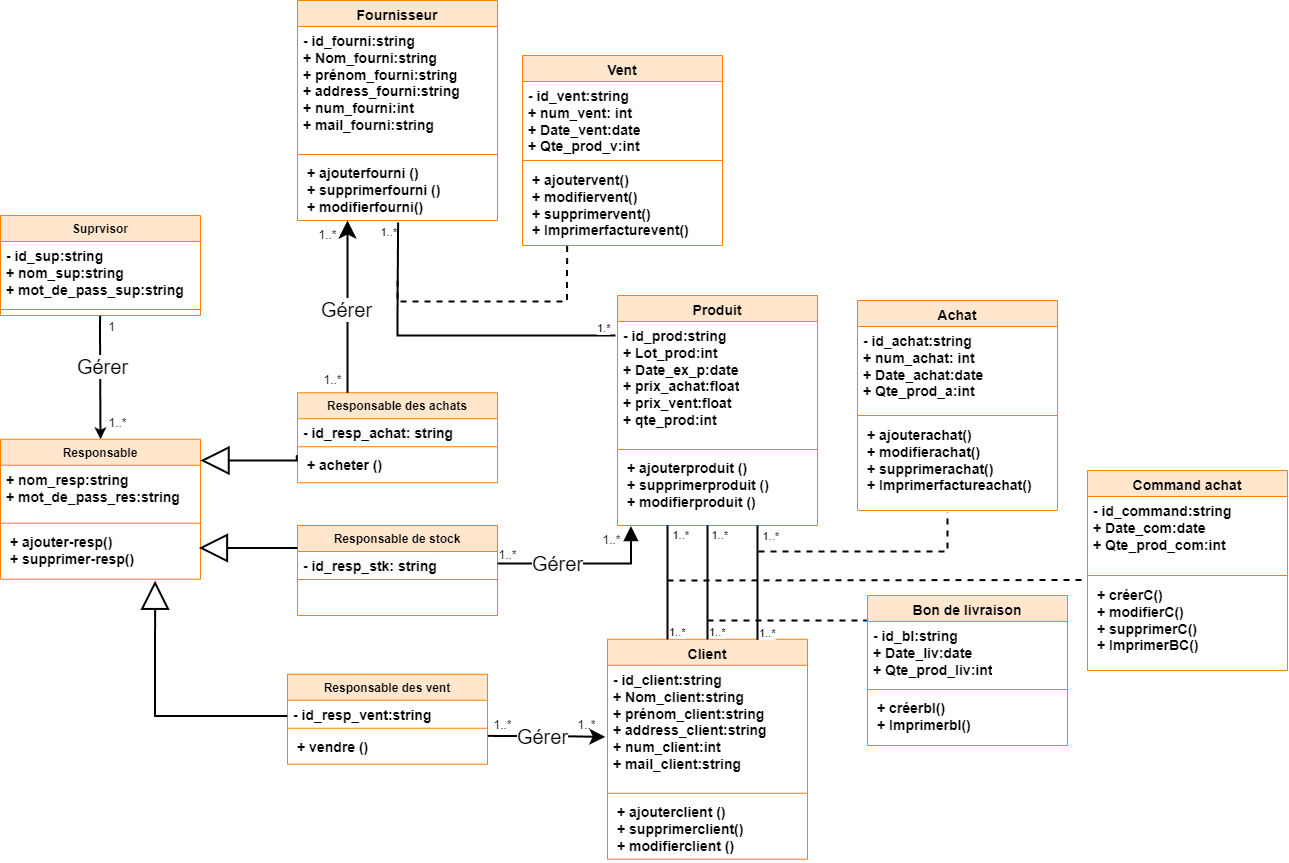
\includegraphics[width=1\textwidth]{images/diagramme de class L.png}
\caption{Diagramme de classe}
\end{figure}
\subsection{Passage du diagramme de classes au modèle relationnel }
Pour passer de diagramme de classe vers le modèle relationnel, nous appliquons les règles suivantes
\newline
\textbf{Règle 1:}Chaque classe devient une table, les attributs de la classe deviennent
les attributs et l’identifiant devient clé primaire pour la table.
\newline
\textbf{Règle 2:}Chaque association 1-1 est prise en compte en incluant la clé primaire
d’une des relations comme clé étrangère dans l’autre relation.
\newline
\textbf{Règle 3:}Chaque association 1-N est prise en compte en incluant la clé comme
clé étrangère dans la relation dont la multiplicité maximale est * la clé primaire
de l’autre relation.
\newline
\textbf{Règle 4:}Chaque association M-N est prise en compte en créant une nouvelle
relation dont la clé primaire est la concaténation des clés primaires de relations
participantes. Les attributs de la classe d’association sont insérés dans cette nouvelle relation si nécessaire.
\newline \phantom{hassane} \newline
En appliquant les règles sur de passage mentionnée dans la partie précédente sur le diagramme de classe suivant (figure: \ref{fig:diag_classl}), on obtient le modèle relationnel qui contient les tables suivantes :
\begin{itemize}
    \item supervisor(\underline{id\_sup},nom\_sup,mot\_de\_pass\_sup,\#id\_resp\_vent,\#id\_resp\_achat \#id\_resp\_stk)
    \item responsable des achats(\underline{id\_resp\_achat},nom\_resp,mot\_de\_pass\_res)
    \item responsable des vent(\underline{id\_resp\_vent},nom\_resp,mot\_de\_pass\_res)
    \item responsable de stock(\underline{id\_resp\_stk},nom\_resp,mot\_de\_pass\_res)
    \item founisseur(\underline{id\_fourni},nom\_fourni,prénom\_fourni,address\_fourni,num\_fourni,mail\_fourni)
    \item client(\underline{id\_client},nom\_client,prénom\_client,address\_client,num\_client,mail\_client)
    \item produit(\underline{id\_prod},lot\_prod,date\_ex\_p,prix\_achat,prix\_vent,qte\_prod)
    \item vent(\underline{id\_vent},num\_vent,date\_vent,qte\_prod\_v,\#id\_fourn,\#id\_prod)
    \item achat(\underline{id\_acha}t,num\_achat,date\_achat,qte\_prod\_a,\#id\_prod,\#id\_client)
    \item command achat(\underline{id\_command},date\_com,qte\_prod\_com,\#id\_prod,\#id\_client)
    \item bon de livraison(\underline{id\_bl},date\_liv,qte\_prod\_liv,\#id\_prod,\#id\_client)
    
\end{itemize}
\section{Conclusion}
La phase de conception a transformé les besoins analytiques en une architecture tangible pour le logiciel de gestion du stock. Le diagramme de classe a défini les structures de données et les relations entre les différents composants du système. Cette phase a assuré que le design technique réponde adéquatement aux exigences fonctionnelles et permette une mise en oeuvre efficace.


%=============================>
\clearpage 
\chapter{Système de recommandation}
\section{Introduction}
Les systèmes de recommandation jouent un rôle crucial dans de nombreuses plateformes en ligne, des sites de commerce électronique aux services de streaming en passant par les réseaux sociaux. Leur objectif principal est de fournir des recommandations personnalisées, ce qui améliore l'expérience utilisateur et stimule l'engagement. Voici quelques points clés à savoir sur ces systèmes.
\section{Comment fonctionnent-ils ?}
\begin{enumerate}
    \item \textbf{Collecte des données:}Les systèmes de recommandation recueillent des données sur les préférences des utilisateurs, telles que les achats précédents, les évaluations, les clics, les recherches, etc.
    \item \textbf{Analyse des données:}En utilisant des algorithmes, ces systèmes analysent les données utilisateur pour trouver des modèles ou des similarités entre utilisateurs et articles.
    \item \textbf{Génération de recommandations:}En se basant sur ces modèles, les systèmes de recommandation prédisent les éléments qui pourraient intéresser un utilisateur donné et leur recommandent ces éléments.
\end{enumerate}
la figure \ref{sr} illustre le processus de recommandation de produits similaires dans un système basé sur les interactions de l'utilisateur. Un produit visualisé par un utilisateur est analysé, et des produits similaires sont identifiés et ensuite recommandés à l'utilisateur.
\begin{figure}[H]
    \centering
    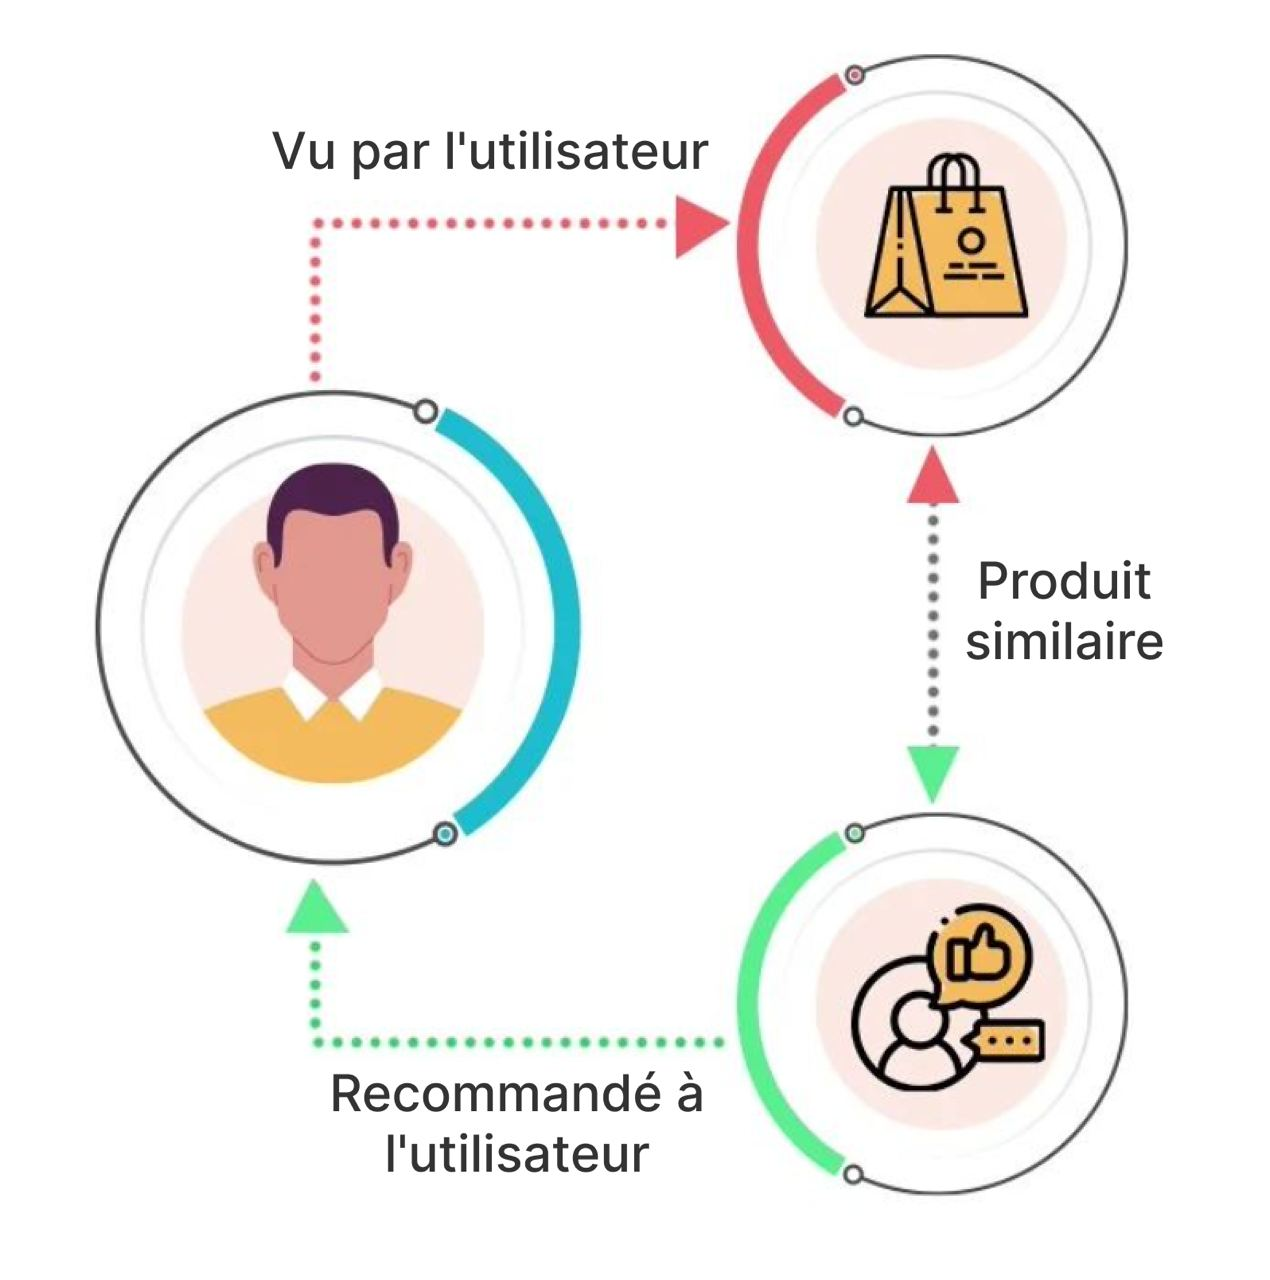
\includegraphics[width=0.5\textwidth]{images/recommendation system.jpg}
    \caption{processus de recommandation}
\end{figure}\label{sr}
\section{Types de systèmes de recommandation}
\begin{enumerate}
    \item \textbf{Filtrage collaboratif:}basé sur le comportement des utilisateurs similaires.
    \item \textbf{Filtrage basé sur le contenu:}recommande des éléments similaires à ceux déjà aimés par l'utilisateur.
    \item \textbf{Recommandation hybride:}combinaison de plusieurs méthodes pour des recommandations plus précises.
\end{enumerate}
\section{Objectifs du Système de Recommandation}
\begin{itemize}
    \item \textbf{Amélioration de l'expérience utilisateur:} Fournir des recommandations personnalisées pour chaque utilisateur afin d'améliorer la satisfaction et l'engagement.
    \item \textbf{Augmentation des ventes:} Stimuler les ventes en proposant des produits pertinents susceptibles d'intéresser les utilisateurs.
    \item \textbf{Gestion du cold-start:} Adresser le problème des nouveaux utilisateurs et des nouveaux produits pour lesquels il y a peu ou pas de données d'interaction.
\end{itemize}
\section{L'Impact des Recommandations Personnalisées}
Ajouter un système de recommandation à notre systeme “EASYCOM” peut avoir plusieurs impacts importants et bénéfiques
\begin{enumerate}
    \item \textbf{Amélioration de l'expérience utilisateur} \begin{itemize}
             \item \textbf{Personnalisation:}les recommandations personnalisées rendent l'expérience utilisateur plus agréable et pertinente, augmentant ainsi l'engagement et la satisfaction des utilisateurs.
             \item \textbf{Découverte de produits:}les utilisateurs peuvent découvrir des produits qu'ils n'auraient pas trouvés autrement, augmentant la variété de leur expérience d'achat.
            \end{itemize}
    \item \textbf{Augmentation des ventes et des revenus} \begin{itemize}
        \item \textbf{Upselling et cross-selling:}les recommandations peuvent inciter les utilisateurs à acheter des produits complémentaires ou plus chers, augmentant ainsi le panier moyen
        \item \textbf{Conversion:}des recommandations bien placées et pertinentes peuvent convertir les visiteurs en acheteurs plus efficacement.
    \end{itemize}
    \item \textbf{Fidélisation des clients} \begin{itemize}
        \item \textbf{Engagement continu:}les utilisateurs sont plus susceptibles de revenir sur l'application si elle continue de leur proposer des produits pertinents et intéressants.
        \item \textbf{Loyauté:}une expérience personnalisée et agréable peut fidéliser les clients, les incitant à revenir régulièrement.
    \end{itemize}
    \item \textbf{Optimisation du stock et des inventaires} \begin{itemize}
        \item \textbf{Gestion des stocks:}En recommandant des produits en surstock, l'application peut aider à équilibrer l'inventaire.
        \item \textbf{Prévisions de demande:}Les données sur les produits recommandés et achetés peuvent aider à prévoir les tendances de demande et à optimiser les commandes de stock.
    \end{itemize}
    \item \textbf{Avantage concurrentiel} \begin{itemize}
        \item \textbf{Différenciation:}Offrir une expérience personnalisée peut distinguer l'application des concurrents qui n'ont pas de système de recommandation.
        \item \textbf{Innovation:}Un système de recommandation peut positionner l'application comme innovante et à la pointe de la technologie
    \end{itemize}
\end{enumerate}
\section{Utilisation de LightFM}
LightFM est une bibliothèque Python populaire pour la construction de systèmes de recommandation. Elle combine les avantages du filtrage collaboratif et du filtrage basé sur le contenu.
\section{Pourquoi LightFM ?}
\subsection*{Points Forts de LightFM}
\textbf{1.Flexibilité et Polyvalence}
\begin{itemize}
    \item \textbf{Approche Hybride:}LightFM combine les méthodes de filtrage collaboratif et de filtrage basé sur le contenu, ce qui permet de tirer parti des interactions utilisateur-élément et des caractéristiques des articles pour offrir des recommandations précises.
    \item \textbf{Support de différentes pertes:}LightFM supporte plusieurs fonctions de perte (WARP, BPR, Logistic), permettant de choisir celle qui convient le mieux à nos objectifs.
\end{itemize}
\phantom{2.2}\textbf{2.Performance et Scalabilité}
\begin{itemize}
    \item \textbf{Efficacité de l'entraînement:}LightFM est optimisé pour être rapide et efficace, même sur des jeux de données volumineux.
    \item \textbf{Précision des recommandations:}En utilisant des techniques de factorisation matricielle avancées, LightFM offre des recommandations de haute qualité, ce qui se traduit par une meilleure précision et un meilleur rappel.
\end{itemize}
\phantom{2.2}\textbf{3.Facilité d'intégration et d'utilisation}
\begin{itemize}
    \item \textbf{Interface simple:}La bibliothèque est conçue pour être facile à utiliser, avec une API claire et intuitive.
    \item \textbf{Compatibilité:}LightFM s'intègre facilement avec d'autres outils et bibliothèques Python, facilitant ainsi son intégration dans notre pipeline existant.
\end{itemize}

\section{Méthode de Calcul du Modèle LightFM}
LightFM utilise des techniques de factorisation matricielle combinées à des approches de filtrage collaboratif et de filtrage basé sur le contenu. Cette section détaille les méthodes de calcul sous-jacentes à ce modèle.
\subsection{Factorisation Matricielle}
La factorisation matricielle est au cœur de LightFM. Elle consiste à décomposer la matrice d'interactions utilisateur-élément \( R \) en deux matrices de rang inférieur : une matrice utilisateur \( U \) et une matrice élément \( V \).
\begin{itemize}
    \item Matrice des interactions \( R \):Représente les interactions (par exemple, évaluations, clics, achats) entre les utilisateurs et les articles.
    \item Matrice utilisateur \( U \):Représente les facteurs latents des utilisateurs.
    \item Matrice élément \( V \):Représente les facteurs latents des articles.
\end{itemize}
L'objectif est de trouver \( U \) et \( V \) telles que \( R \approx UV^T \).
\subsection{Fonction de Perte}
LightFM supporte plusieurs fonctions de perte pour optimiser la factorisation, notamment WARP (Weighted Approximate-Rank Pairwise), BPR (Bayesian Personalized Ranking), et la perte logistique. Nous nous concentrerons sur la perte WARP, qui est souvent utilisée en pratique pour les systèmes de recommandation.
\newline
\textbf{Perte WARP} :
\newline
La perte WARP est conçue pour optimiser directement le rang des éléments recommandés. Elle favorise les éléments bien classés par rapport aux éléments mal classés pour chaque utilisateur.
\newline
Formellement, pour chaque interaction observée \((u, i)\), où \(u\) est un utilisateur et \(i\) est un article avec une interaction positive, la perte WARP est définie comme :

\[
\text{WARP}(u, i) = \sum_{j \in J} \max(0, 1 - \hat{r}_{ui} + \hat{r}_{uj})
\]

Où :

\begin{itemize}
    \item \(\hat{r}_{ui}\) est le score prédit pour l'interaction entre l'utilisateur \(u\) et l'article \(i\).
    \item \(\hat{r}_{uj}\) est le score prédit pour l'interaction entre l'utilisateur \(u\) et un article \(j\) négatif (non observé).
    \item \(J\) est l'ensemble des échantillons d'articles négatifs.
\end{itemize}

Le but est de maximiser la différence entre les scores des interactions positives et négatives, en minimisant la fonction de perte.
\subsection{Optimisation}
L'optimisation est réalisée en utilisant une approche de descente de gradient stochastique. LightFM met à jour les matrices \( \mathbf{U} \) et \( \mathbf{V} \) de manière itérative pour minimiser la fonction de perte choisie.

\begin{enumerate}
    \item \textbf{Initialisation}:Les matrices \( \mathbf{U} \) et \( \mathbf{V} \) sont initialisées avec des valeurs aléatoires.
    \item \textbf{Descente de Gradient}
    \begin{itemize}
        \item Pour chaque interaction positive \( (u, i) \), un élément négatif \( j \) est échantillonné.
        \item Les gradients des paramètres \( \mathbf{U}_u \) et \( \mathbf{V}_i \) sont calculés et utilisés pour mettre à jour les vecteurs latents.
    \end{itemize}
\end{enumerate}
\subsection{Prédiction}
Les scores prédits pour les interactions utilisateur-élément sont calculés comme le produit scalaire des vecteurs latents de l'utilisateur et de l'article :

\[
\hat{r}_{ui} = U_u \cdot V_i^T
\]

Où \(U_u\) est le vecteur de facteurs latents de l'utilisateur \(u\) et \(V_i\) est le vecteur de facteurs latents de l'article \(i\).

\section{Implémentation en LightFM}
Voici comment ces concepts sont implémentés dans LightFM
\subsection{Chargement des données et création du modèle}
\begin{figure} [H]
    \centering
    \includegraphics[width=15.742708333cm , height = 9cm , angle=360]{images/Chargement des données.png}
    \caption{Chargement des données et création du modèle}
    \label{fig:cdd}
\end{figure}
\subsection{Évaluation du modèle}
\begin{figure} [H]
    \centering
    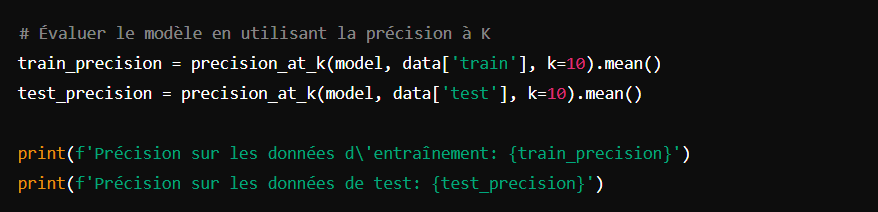
\includegraphics[width=15.742708333cm , height = 5cm , angle=360]{images/Évaluation du modèle.png}
    \caption{Évaluation du modèle}
    \label{fig:Évaluation du modèle}
\end{figure}
\subsection{Génération de recommandations}
\begin{figure} [H]
    \centering
    \includegraphics[width=15.742708333cm , height = 14cm , angle=360]{images/Génération de recommandations.png}
    \caption{Génération de recommandations}
    \label{fig:Génération de recommandations}
\end{figure}
\section{Conclusion}
Ce chapitre a exploré le fonctionnement des systèmes de recommandation, leurs types, et leurs objectifs. L'accent a été mis sur l'utilisation de LightFM pour créer un système de recommandation performant. Les raisons du choix de LightFM, ainsi que les méthodes de calcul du modèle, ont été détaillées, montrant comment ce système peut personnaliser les recommandations de manière efficace. Cette analyse a démontré l'importance des systèmes de recommandation dans l'amélioration de l'expérience utilisateur et la personnalisation des services.


%====================================>
\chapter{Implémentation}
\section{Introduction}
Dans ce chapitre nous allons aborder la dernière phase de notre projet qui est « l’implémentation». Donc, nous présentons les différents langages, outils et bibliothèques utilisées pour sa réalisation, ensuite nous présenterons quelque interfaces de notre système.
\section{Environnement de développement }
Dans cette partie on présentera l'environnement matériel et logiciel, ainsi que les outils de développement. 
\subsection{Environnement Matériel }
Pour développer notre système nous avons utilisé les ordinateurs portables dont on cite les caractéristiques suivantes :  
\begin{table}[h!]
    \centering
    \begin{tabular}{|c|c|c|c|c|}
    \hline
        Modèle de & Processeur & RAM & Disque dur & Système  \\
        l’ordinateur & & & & d’exploitation \\
        \hline
        &&&&\\
         Dell inspiron & Intel(R) Core(TM)   & 4,00  & 512 GO & Windows 10 pro  \\
         3543 & i5-5200U CPU & GO  & HDD & - 64 bits \\
         & @ 2.20GHz   2.20 GHz & & &\\
         &&&&\\
         \hline
        &&&&\\
         dell latitude  & Intel(R) Core(TM)  & 8,00 & 256 GO & Windows 11 pro  \\
         5400 & i5-8265U CPU @ & GO & SSD & – 64 bits \\
         & 1.60GHZ 1.80GHZ & & &\\
         &&&&\\
         \hline
         &&&&\\
         HP ProBook  & Intel(R) Core(TM)   & 4,00& 128 GO  & Windows 10 pro  \\
         430 G3 & i5-6200U CPU @ & GO & SSD & – 64 bits\\
         & 2.30GHZ 2.30GHZ & & &\\
         &&&&\\
         \hline
    \end{tabular}
    \caption{Environnement matériel de développement de le système}
    \label{tab:materiel}
\end{table}
\subsection{Environnement logiciel }
Les outils utilisés pour le développement du projet concernant :
\subsubsection{ Outil de modélisation UML }
\textbf{draw.io:}Draw.io est un outil en ligne gratuit pour créer et partager des diagrammes, tels que des organigrammes, des diagrammes de flux et des cartes mentales. Il offre une interface intuitive, des options de collaboration en temps réel et des intégrations avec divers services de stockage cloud.\cite{drawio}
\begin{figure}[H]\label{fig:draw.io}
    \centering
    \includegraphics[width=3cm , height = 2.5cm , angle=360]{images/drawio.png}
    \caption{draw.io}
    \end{figure}
\subsubsection{langage de développement }
Pour développer notre application nous avons utilisé les langages suivants :
\newline\textbf{JavaScript:}JavaScript (JS) est un langage de programmation interprété et orienté objet principalement utilisé pour le développement web. Il permet de créer des pages web interactives et dynamiques en manipulant le contenu HTML et CSS.\cite{js}
\begin{figure}[H]\label{fig:js}
    \centering
    \includegraphics[width=3cm , height = 2.5cm , angle=360]{images/Javascript.png}
    \caption{JavaScript}
    \end{figure}
\textbf{CSS:}CSS (Cascading Style Sheets), c’est un langage qui vient compléter le HTML, son rôle principal est de traiter la mise en forme du contenu d’une page HTML.\cite{css}
\begin{figure}[H]\label{fig:css}
    \centering
    \includegraphics[width=3cm , height = 3cm , angle=360]{images/css.png}
    \caption{css}
    \end{figure}
\newpage
\textbf{nodejs:}Node.js est un environnement d'exécution JavaScript côté serveur. Il permet d'exécuter du code JavaScript en dehors d'un navigateur, facilitant le développement de serveurs web et d'applications réseau rapides et évolutives grâce à son modèle asynchrone et basé sur les événements.\cite{nodejs}
\begin{figure}[H]\label{fig:nodejs}
    \centering
    \includegraphics[width=4cm , height = 2.5cm , angle=360]{images/nodejs.png}
    \caption{nodejs}
    \end{figure}
\textbf{SQLite:}SQLite est une base de données relationnelle légère, sans serveur, stockée dans un fichier unique. Elle est idéale pour les applications embarquées et mobiles.\cite{sqlite}
    \begin{figure}[H]\label{fig:nodejs}
        \centering
        \includegraphics[width=4cm , height = 2.5cm , angle=360]{images/SQLite370.png}
        \caption{nodejs}
        \end{figure}
\subsubsection{bibliothèques utilisées}
\begin{itemize}
    \item \textbf{Reactjs:}ReactJS est une bibliothèque JavaScript développée par Facebook pour construire des interfaces utilisateur. Elle permet de créer des composants réutilisables et dynamiques, facilitant le développement d'applications web interactives et performantes.\cite{reactjs}
    \item \textbf{Electron.js:}Electron.js est un framework permettant de créer des applications de bureau multiplateformes en utilisant des technologies web comme JavaScript, HTML et CSS. Développé par GitHub, il combine Chromium et Node.js, permettant aux développeurs web de créer des applications natives pour Windows, macOS et Linux.\cite{electron}
    \item \textbf{Tailwind:}Tailwind CSS est un framework CSS utilitaire permettant de créer rapidement des interfaces utilisateur personnalisées en utilisant des classes prédéfinies.\cite{tailwind}
    \item \textbf{Bootstrap:}Bootstrap est un framework CSS populaire pour développer des sites web et des applications réactifs et mobiles en utilisant des composants préconçus et un système de grille flexible.\cite{Bootstrap}
    \item \textbf{React native:}React Native est un framework open-source développé par Facebook, permettant de créer des applications mobiles pour iOS et Android en utilisant JavaScript et React.\cite{reactn}
    \item \textbf{Express.js:}Express est un framework web minimaliste et flexible pour Node.js, utilisé pour créer des applications web et des API robustes et performantes.\cite{express}
    \item \textbf{matreal design:}Material Design est un langage de conception développé par Google, visant à créer des interfaces utilisateur intuitives et cohérentes en utilisant des principes de design basés sur la physique, la lumière et les ombres pour offrir une expérience utilisateur riche et immersive.\cite{matreal}
\end{itemize}






\subsubsection{Outils de développement }
Pour développer notre application nous avons utiliser les logiciels suivants :
\newline\textbf {Visual Studio Code :}Visual Studio Code est un éditeur de code source gratuit et multiplateforme développé par Microsoft. Il offre des fonctionnalités comme la coloration syntaxique, le débogage intégré, le contrôle de version Git et une vaste bibliothèque d'extensions pour supporter divers langages de programmation et outils de développement.\cite{vscode}
\begin{figure}[H]\label{fig:vscode}
    \centering
    \includegraphics[width=4cm , height = 2.5cm , angle=360]{images/vscode.png}
    \caption{visual Studio code}
    \end{figure}
\textbf {Git :}Git est un système de contrôle de version distribué gratuit et open source conçu pour tout gérer, des petits aux très grands projets, avec rapidité et efficacité, facile à apprendre et a une petite empreinte avec des performances ultra-rapides. Il surclasse les outils SCM tels que Subversion, CVS, Perforce et ClearCase avec des fonctionnalités telles que la création de branches locales bon marché, des zones de mise en scène pratiques et plusieurs flux de travail. \cite{git}
\begin{figure}[H]
    \centering
    \includegraphics[width=3cm , height = 2.5cm , angle=360]{images/git.jpg}
    \caption{Git}
    \label{fig:git}
\end{figure}
  \textbf {Github  :}GitHub est une plateforme web de contrôle de versions et de collaboration pour les développeurs de logiciels. \cite{github}
  \begin{figure} [H]
    \centering
    \includegraphics[width=2.5cm , height = 2cm , angle=360]{images/github.png}
    \caption{Github}
    \label{fig:github}
\end{figure}
\textbf{Figma:} c'est un éditeur de graphiques vectoriels et un outil de prototypage. Il est principalement basé sur le web, avec des fonctionnalités hors ligne supplémentaires activées par des applications de bureau pour macOS et Windows. L'ensemble des fonctionnalités de Figma est axé sur l'utilisation dans la conception de l'interface utilisateur et de l'expérience utilisateur, en mettant l'accent sur la collaboration en temps réel. \cite{figma}
  \begin{figure}[H] 
    \centering
    \includegraphics[width=1.5cm , height = 2cm , angle=360]{images/figma.png}
    \caption{Figma}
    \label{fig:figma}
\end{figure}
\section{MongoDB} MongoDB est une base de données NoSQL orientée documents. Elle stocke les données dans des documents JSON (ou BSON), ce qui permet une flexibilité et une évolutivité accrues par rapport aux bases de données relationnelles traditionnelles. MongoDB est utilisé pour des applications nécessitant une gestion de grandes quantités de données non structurées ou semi-structurées.
\begin{figure}[H] 
    \centering
    \includegraphics[width=7cm , height = 2cm , angle=360]{images/mongodb.png}
    \caption{MongoDB}
    \label{fig:MongoDB}
\end{figure}
\subsection{MongoDB atlas}
MongoDB Atlas est une base de données MongoDB entièrement gérée dans le cloud. Elle permet de déployer, gérer et faire évoluer des clusters MongoDB sur les principaux fournisseurs de cloud (AWS, Google Cloud, Azure). Atlas offre des fonctionnalités comme la sauvegarde automatisée, la restauration, le monitoring et des mesures de sécurité avancées pour garantir la haute disponibilité et la performance de vos applications.\cite{atlas}
\subsection{MongoDB Compass }
MongoDB Compass est une interface graphique pour MongoDB qui permet d'explorer et de manipuler visuellement les données, de créer des requêtes, d'analyser les schémas, et de surveiller les performances de la base de données.
\newline \phantom{hassane} \newline
La figure (\ref{fig:stock}) représente interface de MongoDB atlas de notre système :
\begin{figure} [H]
    \centering
    \includegraphics[width=15.742708333cm , height = 9cm , angle=360]{images/monogatlas.png}
    \caption{MongoDB atlas}
    \label{fig:stock}
\end{figure}
La figure (\ref{fig:compass}) représente interface de MongoDB Compass de notre système :
\begin{figure} [H]
    \centering
    \includegraphics[width=15.742708333cm , height = 9cm , angle=360]{images/mongodb db.png}
    \caption{MongoDB Compass}
    \label{fig:compass}
\end{figure}
La figure (\ref{fig:db}) représente interface de notre DataBase :
\begin{figure} [H]
    \centering
    \includegraphics[width=15.742708333cm , height = 9cm , angle=360]{images/easycomdb.png}
    \caption{DataBase}
    \label{fig:db}
\end{figure}
\section{Présentation de notre logo}
Notre idée pour le logo est le mot \textbf{"EASYCOM"} et un colis en mouvement rapide, symbolisant la rapidité et la simplicité que notre système apporte à l'écosystème
\begin{figure}[H] 
    \centering
    \includegraphics[width=7cm , height = 2cm , angle=360]{images/logo.png}
    \caption{logo}
    \label{fig:logo}
\end{figure}
\section{Conception des interfaces }
Puisque le design joue un rôle important dans la satisfaction de l'utilisateur, nous avons tenu à suivre un processus de conception pour arriver à un design moderne qui assure une utilisation fluide.
 La figure (\ref{fig:processe}) présente notre processus de conception
 
  \begin{figure} [H]
    \centering
    \includegraphics[width=13.335cm , height = 3.59cm , angle=360]{images/processe.png}
    \caption{Processus de conception}
    \label{fig:processe}
\end{figure}
\section{Présentation des interfaces }
Nous allons par la suite présenter certaines interfaces distinctives de Easycom
\subsection{Les interfaces de site web}
\subsubsection{Les interfaces d'accueil}
La page d'accueil permet une gestion facile du commerce. Les utilisateurs peuvent rechercher des produits, devenir grossistes et accéder à des plusieurs d'offres. Les catégories de produits et les meilleures opportunités d'affaires sont facilement accessibles, avec une interface intuitive pour une navigation simplifiée.
  \begin{figure} [H]
    \centering
    \includegraphics[width = 15.319375cm , height = 10cm , angle=360]{images/home 1.png}
    \caption{Les interfaces d'accueil}
    \label{fig:colors}
\end{figure}

\subsubsection{L'interface mieux notés}
Cette page met en avant les produits les mieux notés, permettant aux utilisateurs de découvrir rapidement les articles les plus appréciés. Les options de tri et de filtrage facilitent la recherche personnalisée. Une interface conviviale assure une navigation fluide pour trouver les meilleures affaires.
  \begin{figure} [H]
    \centering
    \includegraphics[width = 15.319375cm , height = 10cm , angle=360]{images/afficher les annonce 1.png}
    \caption{L'interface mieux notés}
    \label{fig:mieux notés}
\end{figure}


\subsubsection{L'interface devenir un vendeur}
Cette page permet aux utilisateurs de s'inscrire en tant que vendeur. Ils doivent remplir un formulaire détaillé incluant des informations sur leur entreprise, telles que le numéro de carte nationale, le registre de commerce, et les coordonnées de la société. Cette démarche facilite l'intégration des grossistes sur notre plateforme.
  \begin{figure} [H]
    \centering
    \includegraphics[width = 15.319375cm , height = 10cm , angle=360]{images/devenir grossiste 1.png}
    \caption{L'interface devenir un vendeur}
    \label{fig:Devenir un grossiste}
\end{figure}
\subsubsection{L'interface ajouter annonce d’achat}
Cette page de notre site Easycom permet aux acheteurs de publier des annonces de recherche de produits spécifiques. Ils peuvent y ajouter une image, spécifier un titre, choisir une catégorie et un type de produit, indiquer la quantité souhaitée et fournir une description détaillée de leurs besoins. Ces annonces sont visibles uniquement par les grossistes, facilitant ainsi la mise en relation avec des fournisseurs potentiels.
  \begin{figure} [H]
    \centering
    \includegraphics[width = 15.319375cm , height = 10cm , angle=360]{images/ajouter annonce d'achat.png}
    \caption{L'interface ajouter annonce d’achat}
    \label{fig:Ajouter annonce d’achat}
\end{figure}
\subsubsection{L'interface profile vendeur}
Cette page affiche les informations détaillées du vendeur, telles que le nom de la société, les coordonnées et la catégorie de vente, facilitant la gestion des activités commerciales en ligne.
  \begin{figure} [H]
    \centering
    \includegraphics[width = 15.319375cm , height = 10cm , angle=360]{images/profil vendeur.png}
    \caption{L'interface profile vendeur}
    \label{fig:profil vendeur}
\end{figure}



\subsection{Les interfaces d'application}
\subsubsection{Les interfaces d’accueil}
La page d'accueil met en avant des produits populaires et bien notés, permettant aux utilisateurs de découvrir facilement les articles les plus appréciés. Une barre de navigation intuitive en bas de l'écran facilite l'accès aux différentes sections de l'application.
  \begin{figure} [H]
    \centering
    \includegraphics[width=4.5cm , height = 8.5cm , angle=360]{images/app home.png}
    \caption{Les interfaces d'accueil}
    \label{fig:colors}
\end{figure}

\subsubsection{L'interface details annonce}
Après avoir sélectionné un annonce, l'acheteur ou le vendeur accède à cette interface qui lui permet de voir les annonces et d'interagir avec elles. Un bouton \textit{"Ajouter au panier"} permet d'ajouter l'article directement au panier, facilitant ainsi l'expérience d'achat pour l'utilisateur.
  \begin{figure} [H]
    \centering
    \includegraphics[width=4.5cm , height = 8.5cm , angle=360]{images/app annonce.png}
    \caption{Les interfaces d'accueil}
    \label{fig:colors}
\end{figure}

\subsubsection{L'Interface profile}
A partir de cette fenêtre, l'acheteur et le vendeur peuvent consulter les différentes options de profil. Un bouton de déconnexion permet de se déconnecter facilement de l'application.
  \begin{figure} [H]
    \centering
    \includegraphics[width=4.5cm , height = 8.5cm , angle=360]{images/app profil.png}
    \caption{Les interfaces d'accueil}
    \label{fig:colors}
\end{figure}

\subsubsection{l'interface d'authentification et de création de compte}
Les interfaces suivantes représentent les pages d'authentification et de création de compte ainsi que l"interface de réinitialiser le mot de passe.
  \begin{figure} [H]
    \centering
    \includegraphics[width=4.5cm , height = 8.5cm , angle=360]{images/app signin.png}
    \caption{Les interfaces d'accueil}
    \label{fig:colors}
\end{figure}

\subsubsection{L'interface de discussion}
  \begin{figure} [H]
    \centering
    \includegraphics[width=4.5cm , height = 8.5cm , angle=360]{images/app discussiion.png}
    \caption{Les interfaces de discussion}
    \label{fig:colors}
\end{figure}



\subsection{Les interfaces de logiciel}
\subsubsection{L'interface Se connecter}
Cette page de connexion permet aux utilisateurs de s'authentifier sur EasyCom en saisissant leur nom d'utilisateur et leur mot de passe pour accéder aux fonctionnalités de gestion de stock.
  \begin{figure} [H]
    \centering
    \includegraphics[width = 15.319375cm , height = 10cm , angle=360]{images/sign in 1.png}
    \caption{L'interfaces Se connecter}
    \label{fig:se connecter}
\end{figure}
\subsubsection{L'interface Tableau de bord}
Cette page de tableau de bord de notre logiciel présente les ventes, les nouveaux utilisateurs et les commandes en un coup d'œil, avec des graphiques détaillés. La barre latérale permet un accès rapide aux principales sections comme les produits, les commandes et les clients.
  \begin{figure} [H]
    \centering
    \includegraphics[width = 15.319375cm , height = 10cm , angle=360]{images/dashbord 1.png}
    \caption{L'interfaces Tableau de bord}
    \label{fig:Tableau de bordr}
\end{figure}
\subsubsection{L'interface Ajouter produit}
Cette page de notre logiciel permet d'ajouter de nouveaux produits au stock en spécifiant les détails tels que la famille de produit, la marque, le prix d'achat et de vente, ainsi que les taux de remise et la TVA.
  \begin{figure} [H]
    \centering
    \includegraphics[width = 15.319375cm , height = 10cm , angle=360]{images/ajouter produit 1.png}
    \caption{L'interfaces Ajouter produit}
    \label{fig:Ajouter produit}
\end{figure}
\subsubsection{L'interface Commands recus}
Cette page permet de gérer les commandes reçues sur notre site e-commerce. Les utilisateurs peuvent consulter les détails des commandes, vérifier les informations d'achat, et mettre à jour le statut des commandes, assurant une gestion efficace des ventes et des refus.
  \begin{figure} [H]
    \centering
    \includegraphics[width = 15.319375cm , height = 10cm , angle=360]{images/commands recus 1.png}
    \caption{L'interfaces Commands recus}
    \label{fig:Commands recus}
\end{figure}
\subsubsection{L'interface ajouter produit au stock de site}
Cette page de notre logiciel de gestion de stock permet d'ajouter des produits au stock de notre site e-commerce en précisant la quantité et la sous-catégorie. L'interface intuitive facilite la mise à jour en temps réel des inventaires, assurant une gestion efficace et synchronisée entre le logiciel et le site web.
  \begin{figure} [H]
    \centering
    \includegraphics[width = 15.319375cm , height = 10cm , angle=360]{images/ajouter produit au stock de site 1.png}
    \caption{L'interfaces ajouter produit au stock de site}
    \label{fig:ajouter produit au stock de site}
\end{figure}
\section{Conclusion}
Dans ce chapitre, nous avons présenté les différents outils et bibliothèques utilisés pour la réalisation de notre application.
Par la suite, nous avons présenté notre logo et les différentes interfaces. Nous avons pris au sérieux de respecter au maximum, les standards de l’IHM pour la réaliser.
%====================================>
\chapter*{Conclusion Générale}\markboth{Conclusion}{}
Ce mémoire a présenté le développement d'une plateforme Web, application mobile et un logiciel de gestion de stock, visant à améliorer l'écosystème commercial en Algérie. À travers une étude détaillée de ce dernier, nous avons identifié les besoins et les attentes des différents acteurs, y compris les grossistes, détaillants et entreprises.
\newline\newline
L'expression et l'analyse des besoins ont permis de définir clairement les fonctionnalités nécessaires pour notre système. Ces analyses ont mis en lumière les exigences fonctionnelles et techniques cruciales pour la réussite du projet. En nous basant sur ces analyses, nous avons conçu une architecture robuste et des interfaces utilisateur intuitives, assurant une utilisation efficace et une adoption facile par les utilisateurs finaux.
\newline \newline
L'implémentation a été une étape cruciale où les concepts théoriques et les plans de conception ont été transformés en solutions pratiques et fonctionnelles. Cette phase a impliqué des tests rigoureux et des ajustements pour garantir que le système final répond aux attentes et aux besoins identifiés.
\newline \newline
Le projet a réussi à développer une plateforme Web, une application mobile et un logiciel de gestion de stock qui améliorent significativement la communication et les interactions commerciales entre les différents acteurs du marché et qui simplifient la gestion des stocks. En intégrant ces outils dans le quotidien des commerçants, nous avons créé un écosystème plus dynamique, collaboratif et efficient.
\newline \newline
En regardant vers l'avenir, nous prévoyons d'enrichir encore davantage notre plateforme en ajoutant un système de recommandation avancé et en améliorant l'interface utilisateur.
\begin{itemize}
    \item \textbf{Système de recommandation avancé:}Ce système permettra de fournir des recommandations personnalisées aux utilisateurs, basées sur leurs comportements d'achat, leurs préférences et les tendances du marché. Cela aidera les détaillants à mieux anticiper les besoins des clients et à optimiser leurs approvisionnements.
    \item \textbf{Amélioration de l'interface utilisateur:}Nous envisageons de rendre l'interface utilisateur encore plus intuitive et conviviale, en intégrant des fonctionnalités modernes et des designs interactifs. Cela comprendra une navigation simplifiée, des tableaux de bord personnalisables et des outils de visualisation des données améliorés.
    \item \textbf{Systeme de notifications intelligent:}Un système de notifications intelligent sera mis en place pour alerter les utilisateurs en temps réel sur les événements critiques tels que les ruptures de stock, les nouvelles offres, l’état des commandes et les changements de prix. Ce système permettra aux utilisateurs de réagir rapidement aux changements du marché et de prendre des décisions informées.
    \item \textbf{Systeme d’abonement pour les vendeurs:}Après une période de 6 mois d'utilisation gratuite, les vendeurs devront souscrire à un abonnement pour continuer à utiliser notre plateforme. Cet abonnement donnera accès à des fonctionnalités avancées telles que les annonces d'achat, qui signalent les besoins des acheteurs, la réservation de produits auprès d'autres vendeurs et beaucoup d'autres fonctionnalités. Ce modèle d’abonnement encouragera une adoption plus large et une utilisation continue de la plateforme, tout en générant des revenus récurrents pour soutenir le développement futur.
\end{itemize}

Ces améliorations visent à rendre la plateforme non seulement plus performante mais également plus agréable à utiliser, renforçant ainsi l'engagement des utilisateurs et l'efficacité opérationnelle.
\newline \newline 
En conclusion,ce mémoire prouve que l'adoption de technologies numériques et d'outils de gestion novateurs peut avoir un impact significatif sur l'écosystème commercial en Algérie, offrant des solutions modernes aux défis traditionnels et ouvrant la voie à de nouvelles opportunités de croissance et de développement.



 %===================================>
\chapter*{annexe}
\section*{JOURNAL OFFICIEL DE LA  REPUBLIQUE ALGERIENNE N 41(27 juin 2004)}
Art. 3. - il est entendu, au sens de la présente loi par:
\begin{enumerate}
    \item \textbf{agent économique :} tout producteur, commerçant,artisan ou prestataire de services, quel que soit son statut juridique qui exerce dans le cadre de son activité professionnelle habituelle ou en vue de la réalisation de on objet statutaire.
    \item \textbf{Consommateur :} toute personne physique ou morale qui acquiert ou utilise, à des fins excluant tout caractère professionnel, des biens ou des services mis en vente ou offerts
\end{enumerate}
Art. 4. — Le vendeur doit, obligatoirement, informer les clients sur les prix, les tarifs et les conditions de vente des biens et services.\cite{journal41}
\section*{JOURNAL OFFICIEL DE LA  REPUBLIQUE ALGERIENNE N 80(11 décembre 2005)}
  Art. 3.  La facture doit comporter les  mentions, ci-après ,  se  rapportant  à  lagent  économique :
\newline\textbf{1- Mentions relatives au vendeur :}
\begin{itemize}
    \item nom et prénom  (s)  de la personne physique.
    \item dénomination ou raison sociale de la personne morale.
    \item adresse, numéros de téléphone et de fax ainsi que, le cas échéant, ladresse électronique
    \item forme juridique de lagent économique et nature de lactivité.
    \item capital social, le cas échéant.
    \item numéro du registre du commerce.
    \item numéro didentification statistique.
    \item mode de paiement et date  de  règlement de la facture.
    \item date détablissement  et  numéro dordre de la facture.
    \item dénomination  et  quantité  des   biens  vendus   et/ou
    des   prestations  de services  réalisées
    \item prix  unitaire  hors  taxes   des   biens   vendus    et/ou
    des  prestations  de  services réalisées
    \item prix total hors  taxes  des  biens  vendus  et/ou  des
    prestations  de  services réalisées
    \item nature  et   taux   des   taxes   et/ou  droits et/ou
    contributions   dus,  suivant la nature  des  biens  vendus
    et/ou  des prestations de services réalisées.  La taxe   sur
    la   valeur   ajoutée   nest    pas   mentionnée  si lacheteur
    en est exonéré
    \item prix total toutes taxes comprises, libellé en chiffres
    et en lettres
\end{itemize}
\textbf{2- Mentions relatives à lacheteur :}
\begin{itemize}
    \item nom et prénom (s) de la personne physique.
    \item dénomination ou raison sociale de la personne
    morale .
    \item forme juridique et nature de lactivité.
    \item adresse, numéros de téléphone et de fax  ainsi  que,
    le cas échéant, ladresse électronique.
    \item numéro du registre du commerce.
    \item numéro didentification statistique.
\end{itemize}
Si lacheteur est un consommateur, la facture doit mentionner ses nom, prénom (s) et adresse.
\newline
Art. 14.  Il est admis lutilisation du bon de livraison en
 remplacement de la facture  pour les transactions
 commerciales répétitives et régulières portant sur la vente
 de biens à un même client. \cite{journal80}


\printbibliography %Prints bibliography
 \addcontentsline{toc}{chapter}{Bibliographie}

\end{document}
